\documentclass[twoside]{book}

% Packages required by doxygen
\usepackage{fixltx2e}
\usepackage{calc}
\usepackage{doxygen}
\usepackage[export]{adjustbox} % also loads graphicx
\usepackage{graphicx}
\usepackage[utf8]{inputenc}
\usepackage{makeidx}
\usepackage{multicol}
\usepackage{multirow}
\PassOptionsToPackage{warn}{textcomp}
\usepackage{textcomp}
\usepackage[nointegrals]{wasysym}
\usepackage[table]{xcolor}

% Font selection
\usepackage[T1]{fontenc}
\usepackage[scaled=.90]{helvet}
\usepackage{courier}
\usepackage{amssymb}
\usepackage{sectsty}
\renewcommand{\familydefault}{\sfdefault}
\allsectionsfont{%
  \fontseries{bc}\selectfont%
  \color{darkgray}%
}
\renewcommand{\DoxyLabelFont}{%
  \fontseries{bc}\selectfont%
  \color{darkgray}%
}
\newcommand{\+}{\discretionary{\mbox{\scriptsize$\hookleftarrow$}}{}{}}

% Page & text layout
\usepackage{geometry}
\geometry{%
  a4paper,%
  top=2.5cm,%
  bottom=2.5cm,%
  left=2.5cm,%
  right=2.5cm%
}
\tolerance=750
\hfuzz=15pt
\hbadness=750
\setlength{\emergencystretch}{15pt}
\setlength{\parindent}{0cm}
\setlength{\parskip}{3ex plus 2ex minus 2ex}
\makeatletter
\renewcommand{\paragraph}{%
  \@startsection{paragraph}{4}{0ex}{-1.0ex}{1.0ex}{%
    \normalfont\normalsize\bfseries\SS@parafont%
  }%
}
\renewcommand{\subparagraph}{%
  \@startsection{subparagraph}{5}{0ex}{-1.0ex}{1.0ex}{%
    \normalfont\normalsize\bfseries\SS@subparafont%
  }%
}
\makeatother

% Headers & footers
\usepackage{fancyhdr}
\pagestyle{fancyplain}
\fancyhead[LE]{\fancyplain{}{\bfseries\thepage}}
\fancyhead[CE]{\fancyplain{}{}}
\fancyhead[RE]{\fancyplain{}{\bfseries\leftmark}}
\fancyhead[LO]{\fancyplain{}{\bfseries\rightmark}}
\fancyhead[CO]{\fancyplain{}{}}
\fancyhead[RO]{\fancyplain{}{\bfseries\thepage}}
\fancyfoot[LE]{\fancyplain{}{}}
\fancyfoot[CE]{\fancyplain{}{}}
\fancyfoot[RE]{\fancyplain{}{\bfseries\scriptsize Generated by Doxygen }}
\fancyfoot[LO]{\fancyplain{}{\bfseries\scriptsize Generated by Doxygen }}
\fancyfoot[CO]{\fancyplain{}{}}
\fancyfoot[RO]{\fancyplain{}{}}
\renewcommand{\footrulewidth}{0.4pt}
\renewcommand{\chaptermark}[1]{%
  \markboth{#1}{}%
}
\renewcommand{\sectionmark}[1]{%
  \markright{\thesection\ #1}%
}

% Indices & bibliography
\usepackage{natbib}
\usepackage[titles]{tocloft}
\setcounter{tocdepth}{3}
\setcounter{secnumdepth}{5}
\makeindex

% Hyperlinks (required, but should be loaded last)
\usepackage{ifpdf}
\ifpdf
  \usepackage[pdftex,pagebackref=true]{hyperref}
\else
  \usepackage[ps2pdf,pagebackref=true]{hyperref}
\fi
\hypersetup{%
  colorlinks=true,%
  linkcolor=blue,%
  citecolor=blue,%
  unicode%
}

% Custom commands
\newcommand{\clearemptydoublepage}{%
  \newpage{\pagestyle{empty}\cleardoublepage}%
}

\usepackage{caption}
\captionsetup{labelsep=space,justification=centering,font={bf},singlelinecheck=off,skip=4pt,position=top}

%===== C O N T E N T S =====

\begin{document}

% Titlepage & ToC
\hypersetup{pageanchor=false,
             bookmarksnumbered=true,
             pdfencoding=unicode
            }
\pagenumbering{alph}
\begin{titlepage}
\vspace*{7cm}
\begin{center}%
{\Large 3D Game Engine \\[1ex]\large 1.\+2 }\\
\vspace*{1cm}
{\large Generated by Doxygen 1.8.14}\\
\end{center}
\end{titlepage}
\clearemptydoublepage
\pagenumbering{roman}
\tableofcontents
\clearemptydoublepage
\pagenumbering{arabic}
\hypersetup{pageanchor=true}

%--- Begin generated contents ---
\chapter{Namespace Index}
\section{Namespace List}
Here is a list of all namespaces with brief descriptions\+:\begin{DoxyCompactList}
\item\contentsline{section}{\mbox{\hyperlink{namespacerapidxml}{rapidxml}} }{\pageref{namespacerapidxml}}{}
\item\contentsline{section}{\mbox{\hyperlink{namespacese}{se}} }{\pageref{namespacese}}{}
\end{DoxyCompactList}

\chapter{Hierarchical Index}
\section{Class Hierarchy}
This inheritance list is sorted roughly, but not completely, alphabetically\+:\begin{DoxyCompactList}
\item \contentsline{section}{se\+:\+:Abstract\+Asset}{\pageref{classse_1_1_abstract_asset}}{}
\begin{DoxyCompactList}
\item \contentsline{section}{se\+:\+:Mesh}{\pageref{classse_1_1_mesh}}{}
\end{DoxyCompactList}
\item \contentsline{section}{se\+:\+:Abstract\+Renderer}{\pageref{classse_1_1_abstract_renderer}}{}
\begin{DoxyCompactList}
\item \contentsline{section}{se\+:\+:Direct3D}{\pageref{classse_1_1_direct3_d}}{}
\end{DoxyCompactList}
\item \contentsline{section}{se\+:\+:Abstract\+Terrain}{\pageref{classse_1_1_abstract_terrain}}{}
\begin{DoxyCompactList}
\item \contentsline{section}{se\+:\+:Terrain}{\pageref{classse_1_1_terrain}}{}
\end{DoxyCompactList}
\item \contentsline{section}{se\+:\+:Asset\+Loader}{\pageref{classse_1_1_asset_loader}}{}
\item \contentsline{section}{se\+:\+:Bitmap}{\pageref{classse_1_1_bitmap}}{}
\item \contentsline{section}{se\+:\+:Camera\+Controller}{\pageref{classse_1_1_camera_controller}}{}
\item \contentsline{section}{se\+:\+:Debug}{\pageref{classse_1_1_debug}}{}
\item \contentsline{section}{se\+:\+:Entity}{\pageref{classse_1_1_entity}}{}
\begin{DoxyCompactList}
\item \contentsline{section}{se\+:\+:Abstract\+Camera}{\pageref{classse_1_1_abstract_camera}}{}
\begin{DoxyCompactList}
\item \contentsline{section}{se\+:\+:Direct\+X\+Camera}{\pageref{classse_1_1_direct_x_camera}}{}
\end{DoxyCompactList}
\item \contentsline{section}{se\+:\+:Abstract\+Skybox}{\pageref{classse_1_1_abstract_skybox}}{}
\begin{DoxyCompactList}
\item \contentsline{section}{se\+:\+:Skybox}{\pageref{classse_1_1_skybox}}{}
\end{DoxyCompactList}
\end{DoxyCompactList}
\item \contentsline{section}{se\+:\+:F\+P\+S\+Counter}{\pageref{classse_1_1_f_p_s_counter}}{}
\item \contentsline{section}{se\+:\+:Input}{\pageref{classse_1_1_input}}{}
\item \contentsline{section}{se\+:\+:Kernel}{\pageref{classse_1_1_kernel}}{}
\item \contentsline{section}{se\+:\+:Scene}{\pageref{classse_1_1_scene}}{}
\item \contentsline{section}{se\+:\+:Scene\+Manager}{\pageref{classse_1_1_scene_manager}}{}
\item \contentsline{section}{se\+:\+:Timer}{\pageref{classse_1_1_timer}}{}
\item \contentsline{section}{se\+:\+:Transform3f}{\pageref{classse_1_1_transform3f}}{}
\item \contentsline{section}{se\+:\+:Window}{\pageref{classse_1_1_window}}{}
\item \contentsline{section}{se\+:\+:Window\+Handle}{\pageref{structse_1_1_window_handle}}{}
\end{DoxyCompactList}

\chapter{Class Index}
\section{Class List}
Here are the classes, structs, unions and interfaces with brief descriptions\+:\begin{DoxyCompactList}
\item\contentsline{section}{\mbox{\hyperlink{classse_1_1_abstract_asset}{se\+::\+Abstract\+Asset}} }{\pageref{classse_1_1_abstract_asset}}{}
\item\contentsline{section}{\mbox{\hyperlink{classse_1_1_abstract_input}{se\+::\+Abstract\+Input}} }{\pageref{classse_1_1_abstract_input}}{}
\item\contentsline{section}{\mbox{\hyperlink{classse_1_1_abstract_renderer}{se\+::\+Abstract\+Renderer}} }{\pageref{classse_1_1_abstract_renderer}}{}
\item\contentsline{section}{\mbox{\hyperlink{classse_1_1_asset_manager}{se\+::\+Asset\+Manager}} }{\pageref{classse_1_1_asset_manager}}{}
\item\contentsline{section}{\mbox{\hyperlink{classse_1_1_bitmap}{se\+::\+Bitmap}} }{\pageref{classse_1_1_bitmap}}{}
\item\contentsline{section}{\mbox{\hyperlink{classse_1_1_camera}{se\+::\+Camera}} }{\pageref{classse_1_1_camera}}{}
\item\contentsline{section}{\mbox{\hyperlink{classse_1_1_debug}{se\+::\+Debug}} }{\pageref{classse_1_1_debug}}{}
\item\contentsline{section}{\mbox{\hyperlink{classse_1_1_direct3_d}{se\+::\+Direct3D}} }{\pageref{classse_1_1_direct3_d}}{}
\item\contentsline{section}{\mbox{\hyperlink{classse_1_1_direct_input}{se\+::\+Direct\+Input}} }{\pageref{classse_1_1_direct_input}}{}
\item\contentsline{section}{\mbox{\hyperlink{structse_1_1_draw_components}{se\+::\+Draw\+Components}} }{\pageref{structse_1_1_draw_components}}{}
\item\contentsline{section}{\mbox{\hyperlink{classse_1_1_entity}{se\+::\+Entity}} }{\pageref{classse_1_1_entity}}{}
\item\contentsline{section}{\mbox{\hyperlink{classse_1_1_f_p_s_counter}{se\+::\+F\+P\+S\+Counter}} }{\pageref{classse_1_1_f_p_s_counter}}{}
\item\contentsline{section}{\mbox{\hyperlink{classse_1_1_kernel}{se\+::\+Kernel}} }{\pageref{classse_1_1_kernel}}{}
\item\contentsline{section}{\mbox{\hyperlink{classse_1_1_model}{se\+::\+Model}} }{\pageref{classse_1_1_model}}{}
\item\contentsline{section}{\mbox{\hyperlink{classse_1_1_scene}{se\+::\+Scene}} }{\pageref{classse_1_1_scene}}{}
\item\contentsline{section}{\mbox{\hyperlink{classse_1_1_scene_loader}{se\+::\+Scene\+Loader}} }{\pageref{classse_1_1_scene_loader}}{}
\item\contentsline{section}{\mbox{\hyperlink{classse_1_1_scene_manager}{se\+::\+Scene\+Manager}} }{\pageref{classse_1_1_scene_manager}}{}
\item\contentsline{section}{\mbox{\hyperlink{classse_1_1_skybox}{se\+::\+Skybox}} }{\pageref{classse_1_1_skybox}}{}
\item\contentsline{section}{\mbox{\hyperlink{classse_1_1_terrain}{se\+::\+Terrain}} }{\pageref{classse_1_1_terrain}}{}
\item\contentsline{section}{\mbox{\hyperlink{classse_1_1_timer}{se\+::\+Timer}} }{\pageref{classse_1_1_timer}}{}
\item\contentsline{section}{\mbox{\hyperlink{classse_1_1_vector3}{se\+::\+Vector3$<$ T $>$}} }{\pageref{classse_1_1_vector3}}{}
\item\contentsline{section}{\mbox{\hyperlink{structse_1_1_vertex}{se\+::\+Vertex}} }{\pageref{structse_1_1_vertex}}{}
\item\contentsline{section}{\mbox{\hyperlink{classse_1_1_window}{se\+::\+Window}} }{\pageref{classse_1_1_window}}{}
\item\contentsline{section}{\mbox{\hyperlink{classse_1_1_window_manager}{se\+::\+Window\+Manager}} }{\pageref{classse_1_1_window_manager}}{}
\end{DoxyCompactList}

\chapter{File Index}
\section{File List}
Here is a list of all files with brief descriptions\+:\begin{DoxyCompactList}
\item\contentsline{section}{Include/\mbox{\hyperlink{_asset_8h}{Asset.\+h}} }{\pageref{_asset_8h}}{}
\item\contentsline{section}{Include/\mbox{\hyperlink{_asset_loader_8h}{Asset\+Loader.\+h}} }{\pageref{_asset_loader_8h}}{}
\item\contentsline{section}{Include/\mbox{\hyperlink{_bitmap_8h}{Bitmap.\+h}} }{\pageref{_bitmap_8h}}{}
\item\contentsline{section}{Include/\mbox{\hyperlink{_camera_8h}{Camera.\+h}} }{\pageref{_camera_8h}}{}
\item\contentsline{section}{Include/\mbox{\hyperlink{_camera_controller_8h}{Camera\+Controller.\+h}} }{\pageref{_camera_controller_8h}}{}
\item\contentsline{section}{Include/\mbox{\hyperlink{_debug_8h}{Debug.\+h}} }{\pageref{_debug_8h}}{}
\item\contentsline{section}{Include/\mbox{\hyperlink{_entity_8h}{Entity.\+h}} }{\pageref{_entity_8h}}{}
\item\contentsline{section}{Include/\mbox{\hyperlink{_f_p_s_counter_8h}{F\+P\+S\+Counter.\+h}} }{\pageref{_f_p_s_counter_8h}}{}
\item\contentsline{section}{Include/\mbox{\hyperlink{_input_8h}{Input.\+h}} }{\pageref{_input_8h}}{}
\item\contentsline{section}{Include/\mbox{\hyperlink{_kernel_8h}{Kernel.\+h}} }{\pageref{_kernel_8h}}{}
\item\contentsline{section}{Include/\mbox{\hyperlink{_renderer_8h}{Renderer.\+h}} }{\pageref{_renderer_8h}}{}
\item\contentsline{section}{Include/\mbox{\hyperlink{_scene_8h}{Scene.\+h}} }{\pageref{_scene_8h}}{}
\item\contentsline{section}{Include/\mbox{\hyperlink{_scene_manager_8h}{Scene\+Manager.\+h}} }{\pageref{_scene_manager_8h}}{}
\item\contentsline{section}{Include/\mbox{\hyperlink{_skybox_8h}{Skybox.\+h}} }{\pageref{_skybox_8h}}{}
\item\contentsline{section}{Include/\mbox{\hyperlink{std_8h}{std.\+h}} }{\pageref{std_8h}}{}
\item\contentsline{section}{Include/\mbox{\hyperlink{_terrain_8h}{Terrain.\+h}} }{\pageref{_terrain_8h}}{}
\item\contentsline{section}{Include/\mbox{\hyperlink{_timer_8h}{Timer.\+h}} }{\pageref{_timer_8h}}{}
\item\contentsline{section}{Include/\mbox{\hyperlink{_transform_8h}{Transform.\+h}} }{\pageref{_transform_8h}}{}
\item\contentsline{section}{Include/\mbox{\hyperlink{_window_8h}{Window.\+h}} }{\pageref{_window_8h}}{}
\item\contentsline{section}{Include/\+Direct\+X9/\mbox{\hyperlink{_direct3_d_8h}{Direct3\+D.\+h}} }{\pageref{_direct3_d_8h}}{}
\item\contentsline{section}{Include/\+Direct\+X9/\mbox{\hyperlink{_direct_x_camera_8h}{Direct\+X\+Camera.\+h}} }{\pageref{_direct_x_camera_8h}}{}
\item\contentsline{section}{Include/\+Direct\+X9/\mbox{\hyperlink{_direct_x_mesh_8h}{Direct\+X\+Mesh.\+h}} }{\pageref{_direct_x_mesh_8h}}{}
\item\contentsline{section}{Include/\+Direct\+X9/\mbox{\hyperlink{_direct_x_skybox_8h}{Direct\+X\+Skybox.\+h}} }{\pageref{_direct_x_skybox_8h}}{}
\item\contentsline{section}{Include/\+Direct\+X9/\mbox{\hyperlink{_direct_x_terrain_8h}{Direct\+X\+Terrain.\+h}} }{\pageref{_direct_x_terrain_8h}}{}
\end{DoxyCompactList}

\chapter{Namespace Documentation}
\hypertarget{namespacese}{}\section{se Namespace Reference}
\label{namespacese}\index{se@{se}}
\subsection*{Classes}
\begin{DoxyCompactItemize}
\item 
class \mbox{\hyperlink{classse_1_1_abstract_asset}{Abstract\+Asset}}
\item 
class \mbox{\hyperlink{classse_1_1_abstract_camera}{Abstract\+Camera}}
\item 
class \mbox{\hyperlink{classse_1_1_abstract_renderer}{Abstract\+Renderer}}
\item 
class \mbox{\hyperlink{classse_1_1_abstract_skybox}{Abstract\+Skybox}}
\item 
class \mbox{\hyperlink{classse_1_1_abstract_terrain}{Abstract\+Terrain}}
\item 
class \mbox{\hyperlink{classse_1_1_asset_manager}{Asset\+Manager}}
\item 
class \mbox{\hyperlink{classse_1_1_bitmap}{Bitmap}}
\item 
class \mbox{\hyperlink{classse_1_1_camera_controller}{Camera\+Controller}}
\item 
class \mbox{\hyperlink{classse_1_1_debug}{Debug}}
\item 
class \mbox{\hyperlink{classse_1_1_direct3_d}{Direct3D}}
\item 
class \mbox{\hyperlink{classse_1_1_direct_x_camera}{Direct\+X\+Camera}}
\item 
class \mbox{\hyperlink{classse_1_1_entity}{Entity}}
\item 
class \mbox{\hyperlink{classse_1_1_f_p_s_counter}{F\+P\+S\+Counter}}
\item 
class \mbox{\hyperlink{classse_1_1_input}{Input}}
\item 
class \mbox{\hyperlink{classse_1_1_kernel}{Kernel}}
\item 
class \mbox{\hyperlink{classse_1_1_mesh}{Mesh}}
\item 
class \mbox{\hyperlink{classse_1_1_scene}{Scene}}
\item 
class \mbox{\hyperlink{classse_1_1_scene_manager}{Scene\+Manager}}
\item 
class \mbox{\hyperlink{classse_1_1_skybox}{Skybox}}
\item 
class \mbox{\hyperlink{classse_1_1_terrain}{Terrain}}
\item 
class \mbox{\hyperlink{classse_1_1_timer}{Timer}}
\item 
class \mbox{\hyperlink{classse_1_1_transform3f}{Transform3f}}
\item 
struct \mbox{\hyperlink{structse_1_1_window_entity}{Window\+Entity}}
\item 
class \mbox{\hyperlink{classse_1_1_window_manager}{Window\+Manager}}
\end{DoxyCompactItemize}

\chapter{Class Documentation}
\hypertarget{classse_1_1_abstract_asset}{}\section{se\+:\+:Abstract\+Asset Class Reference}
\label{classse_1_1_abstract_asset}\index{se\+::\+Abstract\+Asset@{se\+::\+Abstract\+Asset}}


{\ttfamily \#include $<$Asset.\+h$>$}

Inheritance diagram for se\+:\+:Abstract\+Asset\+:\begin{figure}[H]
\begin{center}
\leavevmode
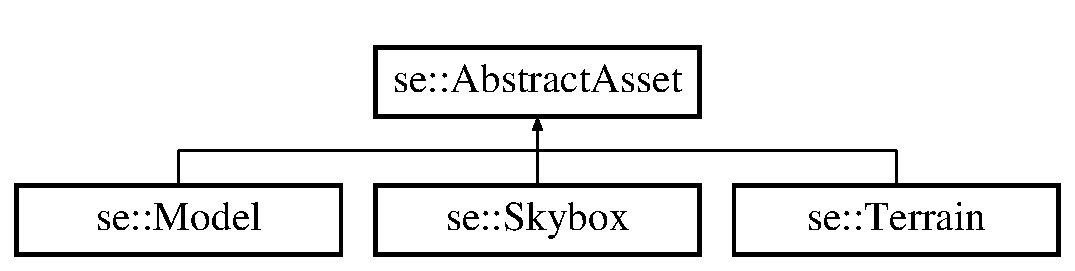
\includegraphics[height=2.000000cm]{classse_1_1_abstract_asset}
\end{center}
\end{figure}
\subsection*{Public Member Functions}
\begin{DoxyCompactItemize}
\item 
virtual void \mbox{\hyperlink{classse_1_1_abstract_asset_ae3f9fb8f5c26ac8ea511e8e21f5bd624}{Create}} ()=0
\item 
virtual void \mbox{\hyperlink{classse_1_1_abstract_asset_afb4dff418acf169d81b6ca5d8c1f6548}{Load}} ()=0
\item 
virtual void \mbox{\hyperlink{classse_1_1_abstract_asset_a1f2fdf75bbeaddec16dc4778063505b7}{Process}} ()=0
\item 
virtual void \mbox{\hyperlink{classse_1_1_abstract_asset_aea97e36f647efdb07a801b6fc468388d}{Release}} ()=0
\end{DoxyCompactItemize}
\subsection*{Protected Attributes}
\begin{DoxyCompactItemize}
\item 
std\+::string \mbox{\hyperlink{classse_1_1_abstract_asset_afa609af58ca8617ef9ab7f6de84e121f}{m\+\_\+path}}
\end{DoxyCompactItemize}


\subsection{Detailed Description}


Definition at line 8 of file Asset.\+h.



\subsection{Member Function Documentation}
\mbox{\Hypertarget{classse_1_1_abstract_asset_ae3f9fb8f5c26ac8ea511e8e21f5bd624}\label{classse_1_1_abstract_asset_ae3f9fb8f5c26ac8ea511e8e21f5bd624}} 
\index{se\+::\+Abstract\+Asset@{se\+::\+Abstract\+Asset}!Create@{Create}}
\index{Create@{Create}!se\+::\+Abstract\+Asset@{se\+::\+Abstract\+Asset}}
\subsubsection{\texorpdfstring{Create()}{Create()}}
{\footnotesize\ttfamily virtual void se\+::\+Abstract\+Asset\+::\+Create (\begin{DoxyParamCaption}{ }\end{DoxyParamCaption})\hspace{0.3cm}{\ttfamily [pure virtual]}}



Implemented in \mbox{\hyperlink{classse_1_1_mesh_a56e2d07f7b642c16e89631796a0d576e}{se\+::\+Mesh}}.

\mbox{\Hypertarget{classse_1_1_abstract_asset_afb4dff418acf169d81b6ca5d8c1f6548}\label{classse_1_1_abstract_asset_afb4dff418acf169d81b6ca5d8c1f6548}} 
\index{se\+::\+Abstract\+Asset@{se\+::\+Abstract\+Asset}!Load@{Load}}
\index{Load@{Load}!se\+::\+Abstract\+Asset@{se\+::\+Abstract\+Asset}}
\subsubsection{\texorpdfstring{Load()}{Load()}}
{\footnotesize\ttfamily virtual void se\+::\+Abstract\+Asset\+::\+Load (\begin{DoxyParamCaption}{ }\end{DoxyParamCaption})\hspace{0.3cm}{\ttfamily [pure virtual]}}



Implemented in \mbox{\hyperlink{classse_1_1_mesh_a17116983a6c6e73770585b72332c5140}{se\+::\+Mesh}}.

\mbox{\Hypertarget{classse_1_1_abstract_asset_a1f2fdf75bbeaddec16dc4778063505b7}\label{classse_1_1_abstract_asset_a1f2fdf75bbeaddec16dc4778063505b7}} 
\index{se\+::\+Abstract\+Asset@{se\+::\+Abstract\+Asset}!Process@{Process}}
\index{Process@{Process}!se\+::\+Abstract\+Asset@{se\+::\+Abstract\+Asset}}
\subsubsection{\texorpdfstring{Process()}{Process()}}
{\footnotesize\ttfamily virtual void se\+::\+Abstract\+Asset\+::\+Process (\begin{DoxyParamCaption}{ }\end{DoxyParamCaption})\hspace{0.3cm}{\ttfamily [pure virtual]}}



Implemented in \mbox{\hyperlink{classse_1_1_mesh_a1ae42a794ee240b5d6a0dd46aa4ea60d}{se\+::\+Mesh}}.

\mbox{\Hypertarget{classse_1_1_abstract_asset_aea97e36f647efdb07a801b6fc468388d}\label{classse_1_1_abstract_asset_aea97e36f647efdb07a801b6fc468388d}} 
\index{se\+::\+Abstract\+Asset@{se\+::\+Abstract\+Asset}!Release@{Release}}
\index{Release@{Release}!se\+::\+Abstract\+Asset@{se\+::\+Abstract\+Asset}}
\subsubsection{\texorpdfstring{Release()}{Release()}}
{\footnotesize\ttfamily virtual void se\+::\+Abstract\+Asset\+::\+Release (\begin{DoxyParamCaption}{ }\end{DoxyParamCaption})\hspace{0.3cm}{\ttfamily [pure virtual]}}



Implemented in \mbox{\hyperlink{classse_1_1_mesh_afde4ccf6665a9b6c7a8f3635dd5139e0}{se\+::\+Mesh}}.



\subsection{Member Data Documentation}
\mbox{\Hypertarget{classse_1_1_abstract_asset_afa609af58ca8617ef9ab7f6de84e121f}\label{classse_1_1_abstract_asset_afa609af58ca8617ef9ab7f6de84e121f}} 
\index{se\+::\+Abstract\+Asset@{se\+::\+Abstract\+Asset}!m\+\_\+path@{m\+\_\+path}}
\index{m\+\_\+path@{m\+\_\+path}!se\+::\+Abstract\+Asset@{se\+::\+Abstract\+Asset}}
\subsubsection{\texorpdfstring{m\+\_\+path}{m\_path}}
{\footnotesize\ttfamily std\+::string se\+::\+Abstract\+Asset\+::m\+\_\+path\hspace{0.3cm}{\ttfamily [protected]}}



Definition at line 15 of file Asset.\+h.



The documentation for this class was generated from the following file\+:\begin{DoxyCompactItemize}
\item 
Include/\mbox{\hyperlink{_asset_8h}{Asset.\+h}}\end{DoxyCompactItemize}

\hypertarget{classse_1_1_abstract_input}{}\section{se\+:\+:Abstract\+Input Class Reference}
\label{classse_1_1_abstract_input}\index{se\+::\+Abstract\+Input@{se\+::\+Abstract\+Input}}


{\ttfamily \#include $<$Input.\+h$>$}

Inheritance diagram for se\+:\+:Abstract\+Input\+:\begin{figure}[H]
\begin{center}
\leavevmode
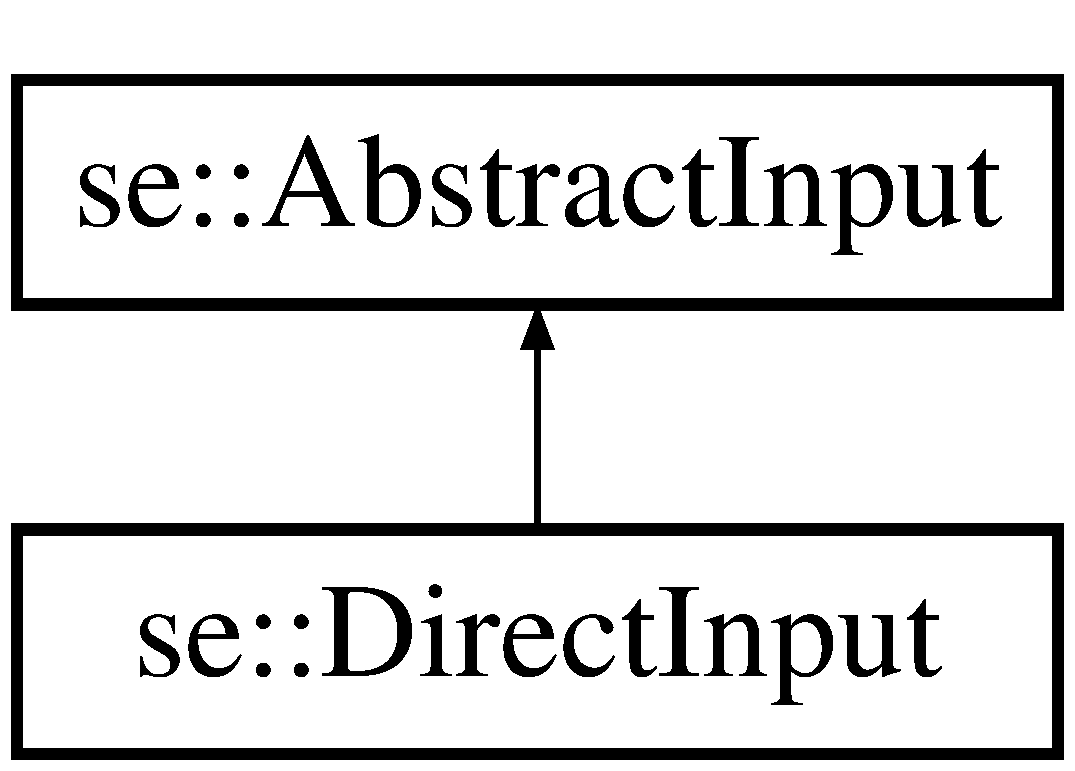
\includegraphics[height=2.000000cm]{classse_1_1_abstract_input}
\end{center}
\end{figure}
\subsection*{Public Member Functions}
\begin{DoxyCompactItemize}
\item 
virtual bool \mbox{\hyperlink{classse_1_1_abstract_input_a6219cdd66247d08f3ca52b2fea305b8d}{Initialize}} (H\+I\+N\+S\+T\+A\+N\+CE h\+Instance, H\+W\+ND h\+Wnd, int screen\+Width, int screen\+Height)=0
\item 
virtual bool \mbox{\hyperlink{classse_1_1_abstract_input_a4375b92281cee63064c898a791ddd1a3}{Is\+Pressed}} (\mbox{\hyperlink{namespacese_a94221cf8f238f1eadbe3ac4b8ac7bc71}{Keyboard\+Key}} key)=0
\item 
virtual void \mbox{\hyperlink{classse_1_1_abstract_input_a7c9b63e9df453d38c035fb9fa91c0d70}{Update}} ()=0
\item 
virtual void \mbox{\hyperlink{classse_1_1_abstract_input_a93673fb3534be8bbc1f495f650064b91}{Get\+Mouse\+Location}} (int \&mouseX, int \&mouseY)=0
\end{DoxyCompactItemize}


\subsection{Detailed Description}
You can use this interface to create your own input handler. 

Definition at line 12 of file Input.\+h.



\subsection{Member Function Documentation}
\mbox{\Hypertarget{classse_1_1_abstract_input_a93673fb3534be8bbc1f495f650064b91}\label{classse_1_1_abstract_input_a93673fb3534be8bbc1f495f650064b91}} 
\index{se\+::\+Abstract\+Input@{se\+::\+Abstract\+Input}!Get\+Mouse\+Location@{Get\+Mouse\+Location}}
\index{Get\+Mouse\+Location@{Get\+Mouse\+Location}!se\+::\+Abstract\+Input@{se\+::\+Abstract\+Input}}
\subsubsection{\texorpdfstring{Get\+Mouse\+Location()}{GetMouseLocation()}}
{\footnotesize\ttfamily virtual void se\+::\+Abstract\+Input\+::\+Get\+Mouse\+Location (\begin{DoxyParamCaption}\item[{int \&}]{mouseX,  }\item[{int \&}]{mouseY }\end{DoxyParamCaption})\hspace{0.3cm}{\ttfamily [pure virtual]}}

Get the mouse location. 

Implemented in \mbox{\hyperlink{classse_1_1_direct_input_a3c097a463a36421a13bf05819c4b681e}{se\+::\+Direct\+Input}}.

\mbox{\Hypertarget{classse_1_1_abstract_input_a6219cdd66247d08f3ca52b2fea305b8d}\label{classse_1_1_abstract_input_a6219cdd66247d08f3ca52b2fea305b8d}} 
\index{se\+::\+Abstract\+Input@{se\+::\+Abstract\+Input}!Initialize@{Initialize}}
\index{Initialize@{Initialize}!se\+::\+Abstract\+Input@{se\+::\+Abstract\+Input}}
\subsubsection{\texorpdfstring{Initialize()}{Initialize()}}
{\footnotesize\ttfamily virtual bool se\+::\+Abstract\+Input\+::\+Initialize (\begin{DoxyParamCaption}\item[{H\+I\+N\+S\+T\+A\+N\+CE}]{h\+Instance,  }\item[{H\+W\+ND}]{h\+Wnd,  }\item[{int}]{screen\+Width,  }\item[{int}]{screen\+Height }\end{DoxyParamCaption})\hspace{0.3cm}{\ttfamily [pure virtual]}}

Initialize the input for the given window instance and handle. 

Implemented in \mbox{\hyperlink{classse_1_1_direct_input_ae8f8c4306ad58f7696548d2c63f01e6f}{se\+::\+Direct\+Input}}.

\mbox{\Hypertarget{classse_1_1_abstract_input_a4375b92281cee63064c898a791ddd1a3}\label{classse_1_1_abstract_input_a4375b92281cee63064c898a791ddd1a3}} 
\index{se\+::\+Abstract\+Input@{se\+::\+Abstract\+Input}!Is\+Pressed@{Is\+Pressed}}
\index{Is\+Pressed@{Is\+Pressed}!se\+::\+Abstract\+Input@{se\+::\+Abstract\+Input}}
\subsubsection{\texorpdfstring{Is\+Pressed()}{IsPressed()}}
{\footnotesize\ttfamily virtual bool se\+::\+Abstract\+Input\+::\+Is\+Pressed (\begin{DoxyParamCaption}\item[{\mbox{\hyperlink{namespacese_a94221cf8f238f1eadbe3ac4b8ac7bc71}{Keyboard\+Key}}}]{key }\end{DoxyParamCaption})\hspace{0.3cm}{\ttfamily [pure virtual]}}

Check if specified Keyboard\+Key is pressed. 

Implemented in \mbox{\hyperlink{classse_1_1_direct_input_ad9669e6834c3fcac489050a82beb71f7}{se\+::\+Direct\+Input}}.

\mbox{\Hypertarget{classse_1_1_abstract_input_a7c9b63e9df453d38c035fb9fa91c0d70}\label{classse_1_1_abstract_input_a7c9b63e9df453d38c035fb9fa91c0d70}} 
\index{se\+::\+Abstract\+Input@{se\+::\+Abstract\+Input}!Update@{Update}}
\index{Update@{Update}!se\+::\+Abstract\+Input@{se\+::\+Abstract\+Input}}
\subsubsection{\texorpdfstring{Update()}{Update()}}
{\footnotesize\ttfamily virtual void se\+::\+Abstract\+Input\+::\+Update (\begin{DoxyParamCaption}{ }\end{DoxyParamCaption})\hspace{0.3cm}{\ttfamily [pure virtual]}}

Update the read key/mouse input. 

Implemented in \mbox{\hyperlink{classse_1_1_direct_input_a863123d7304364a55fd2135f27195500}{se\+::\+Direct\+Input}}.



The documentation for this class was generated from the following file\+:\begin{DoxyCompactItemize}
\item 
D\+:/\+Projects/\+Game\+Engine3\+D/\+Include/\mbox{\hyperlink{_input_8h}{Input.\+h}}\end{DoxyCompactItemize}

\hypertarget{classse_1_1_abstract_renderer}{}\section{se\+:\+:Abstract\+Renderer Class Reference}
\label{classse_1_1_abstract_renderer}\index{se\+::\+Abstract\+Renderer@{se\+::\+Abstract\+Renderer}}


{\ttfamily \#include $<$Renderer.\+h$>$}

Inheritance diagram for se\+:\+:Abstract\+Renderer\+:\begin{figure}[H]
\begin{center}
\leavevmode
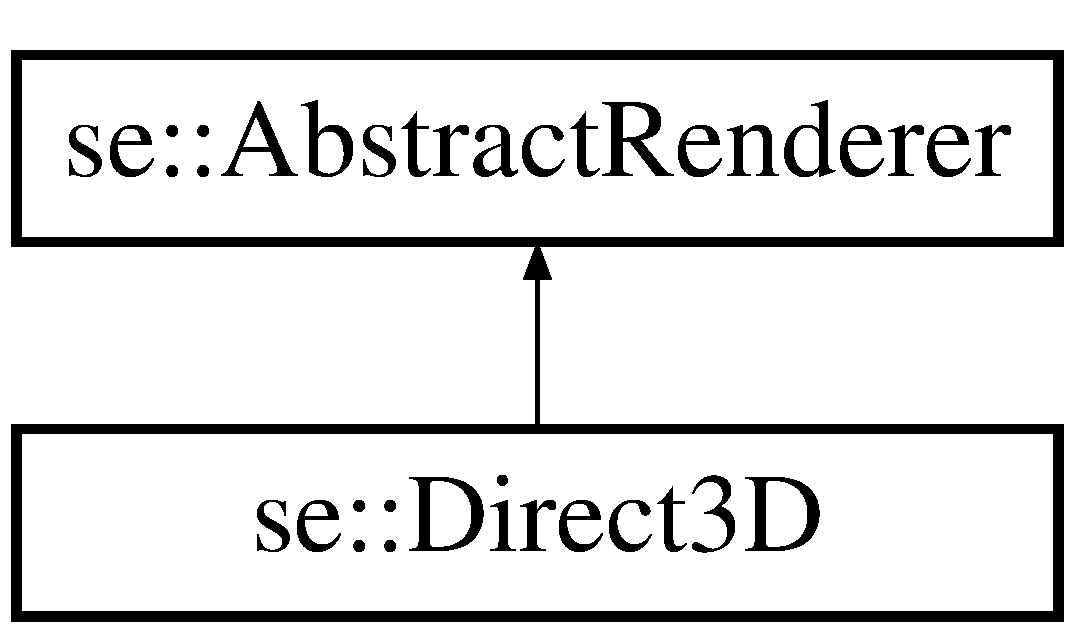
\includegraphics[height=2.000000cm]{classse_1_1_abstract_renderer}
\end{center}
\end{figure}
\subsection*{Public Member Functions}
\begin{DoxyCompactItemize}
\item 
virtual void \mbox{\hyperlink{classse_1_1_abstract_renderer_afdfce8b91028448c17ce27550827f192}{Create}} (H\+W\+ND h\+Wnd)=0
\item 
virtual void \mbox{\hyperlink{classse_1_1_abstract_renderer_aae49e7417663d6a5aca34a2bb37b4b28}{Update}} (float delta)=0
\item 
virtual void \mbox{\hyperlink{classse_1_1_abstract_renderer_a08f813c33edad06bf7d379f8257895e6}{Render}} ()=0
\item 
virtual void \mbox{\hyperlink{classse_1_1_abstract_renderer_a98e35b7db62827580573185ed91b25bb}{Release}} ()=0
\end{DoxyCompactItemize}


\subsection{Detailed Description}


Definition at line 9 of file Renderer.\+h.



\subsection{Member Function Documentation}
\mbox{\Hypertarget{classse_1_1_abstract_renderer_afdfce8b91028448c17ce27550827f192}\label{classse_1_1_abstract_renderer_afdfce8b91028448c17ce27550827f192}} 
\index{se\+::\+Abstract\+Renderer@{se\+::\+Abstract\+Renderer}!Create@{Create}}
\index{Create@{Create}!se\+::\+Abstract\+Renderer@{se\+::\+Abstract\+Renderer}}
\subsubsection{\texorpdfstring{Create()}{Create()}}
{\footnotesize\ttfamily virtual void se\+::\+Abstract\+Renderer\+::\+Create (\begin{DoxyParamCaption}\item[{H\+W\+ND}]{h\+Wnd }\end{DoxyParamCaption})\hspace{0.3cm}{\ttfamily [pure virtual]}}



Implemented in \mbox{\hyperlink{classse_1_1_direct3_d_a316456762829db0614077cccd655e654}{se\+::\+Direct3D}}.

\mbox{\Hypertarget{classse_1_1_abstract_renderer_a98e35b7db62827580573185ed91b25bb}\label{classse_1_1_abstract_renderer_a98e35b7db62827580573185ed91b25bb}} 
\index{se\+::\+Abstract\+Renderer@{se\+::\+Abstract\+Renderer}!Release@{Release}}
\index{Release@{Release}!se\+::\+Abstract\+Renderer@{se\+::\+Abstract\+Renderer}}
\subsubsection{\texorpdfstring{Release()}{Release()}}
{\footnotesize\ttfamily virtual void se\+::\+Abstract\+Renderer\+::\+Release (\begin{DoxyParamCaption}{ }\end{DoxyParamCaption})\hspace{0.3cm}{\ttfamily [pure virtual]}}



Implemented in \mbox{\hyperlink{classse_1_1_direct3_d_ae2979f16a5c35773cf2c243d8e6f90e4}{se\+::\+Direct3D}}.

\mbox{\Hypertarget{classse_1_1_abstract_renderer_a08f813c33edad06bf7d379f8257895e6}\label{classse_1_1_abstract_renderer_a08f813c33edad06bf7d379f8257895e6}} 
\index{se\+::\+Abstract\+Renderer@{se\+::\+Abstract\+Renderer}!Render@{Render}}
\index{Render@{Render}!se\+::\+Abstract\+Renderer@{se\+::\+Abstract\+Renderer}}
\subsubsection{\texorpdfstring{Render()}{Render()}}
{\footnotesize\ttfamily virtual void se\+::\+Abstract\+Renderer\+::\+Render (\begin{DoxyParamCaption}{ }\end{DoxyParamCaption})\hspace{0.3cm}{\ttfamily [pure virtual]}}



Implemented in \mbox{\hyperlink{classse_1_1_direct3_d_af4e167f88160d79fc66b4d65694b536a}{se\+::\+Direct3D}}.

\mbox{\Hypertarget{classse_1_1_abstract_renderer_aae49e7417663d6a5aca34a2bb37b4b28}\label{classse_1_1_abstract_renderer_aae49e7417663d6a5aca34a2bb37b4b28}} 
\index{se\+::\+Abstract\+Renderer@{se\+::\+Abstract\+Renderer}!Update@{Update}}
\index{Update@{Update}!se\+::\+Abstract\+Renderer@{se\+::\+Abstract\+Renderer}}
\subsubsection{\texorpdfstring{Update()}{Update()}}
{\footnotesize\ttfamily virtual void se\+::\+Abstract\+Renderer\+::\+Update (\begin{DoxyParamCaption}\item[{float}]{delta }\end{DoxyParamCaption})\hspace{0.3cm}{\ttfamily [pure virtual]}}



Implemented in \mbox{\hyperlink{classse_1_1_direct3_d_a39934c194406f108a992d82a4d265381}{se\+::\+Direct3D}}.



The documentation for this class was generated from the following file\+:\begin{DoxyCompactItemize}
\item 
Include/\mbox{\hyperlink{_renderer_8h}{Renderer.\+h}}\end{DoxyCompactItemize}

\hypertarget{classse_1_1_asset_manager}{}\section{se\+:\+:Asset\+Manager Class Reference}
\label{classse_1_1_asset_manager}\index{se\+::\+Asset\+Manager@{se\+::\+Asset\+Manager}}


{\ttfamily \#include $<$Asset\+Manager.\+h$>$}

\subsection*{Public Member Functions}
\begin{DoxyCompactItemize}
\item 
void \mbox{\hyperlink{classse_1_1_asset_manager_aee43a38dbf19e852fed3f222808277af}{Add\+Asset}} (const std\+::string \&name, \mbox{\hyperlink{classse_1_1_abstract_asset}{Abstract\+Asset}} $\ast$asset)
\item 
void \mbox{\hyperlink{classse_1_1_asset_manager_a3cd3506b7003d63adbd1cd0f94c8931e}{Release\+Asset}} (const std\+::string \&name)
\item 
std\+::unordered\+\_\+map$<$ std\+::string, \mbox{\hyperlink{classse_1_1_abstract_asset}{Abstract\+Asset}} $\ast$ $>$ \mbox{\hyperlink{classse_1_1_asset_manager_adaa14ad4d80b328f2204543d788c6a28}{Get\+Asset\+List}} ()
\end{DoxyCompactItemize}
\subsection*{Static Public Member Functions}
\begin{DoxyCompactItemize}
\item 
static \mbox{\hyperlink{classse_1_1_asset_manager}{Asset\+Manager}} $\ast$ \mbox{\hyperlink{classse_1_1_asset_manager_abcccad608538c6ddeb223c259089d468}{Get\+Instance}} ()
\end{DoxyCompactItemize}


\subsection{Detailed Description}
With this manager you can add assets and get and release added assets 

Definition at line 12 of file Asset\+Manager.\+h.



\subsection{Member Function Documentation}
\mbox{\Hypertarget{classse_1_1_asset_manager_aee43a38dbf19e852fed3f222808277af}\label{classse_1_1_asset_manager_aee43a38dbf19e852fed3f222808277af}} 
\index{se\+::\+Asset\+Manager@{se\+::\+Asset\+Manager}!Add\+Asset@{Add\+Asset}}
\index{Add\+Asset@{Add\+Asset}!se\+::\+Asset\+Manager@{se\+::\+Asset\+Manager}}
\subsubsection{\texorpdfstring{Add\+Asset()}{AddAsset()}}
{\footnotesize\ttfamily void se\+::\+Asset\+Manager\+::\+Add\+Asset (\begin{DoxyParamCaption}\item[{const std\+::string \&}]{name,  }\item[{\mbox{\hyperlink{classse_1_1_abstract_asset}{Abstract\+Asset}} $\ast$}]{asset }\end{DoxyParamCaption})}

Add an asset with a name to refer it by \mbox{\Hypertarget{classse_1_1_asset_manager_adaa14ad4d80b328f2204543d788c6a28}\label{classse_1_1_asset_manager_adaa14ad4d80b328f2204543d788c6a28}} 
\index{se\+::\+Asset\+Manager@{se\+::\+Asset\+Manager}!Get\+Asset\+List@{Get\+Asset\+List}}
\index{Get\+Asset\+List@{Get\+Asset\+List}!se\+::\+Asset\+Manager@{se\+::\+Asset\+Manager}}
\subsubsection{\texorpdfstring{Get\+Asset\+List()}{GetAssetList()}}
{\footnotesize\ttfamily std\+::unordered\+\_\+map$<$std\+::string, \mbox{\hyperlink{classse_1_1_abstract_asset}{Abstract\+Asset}}$\ast$$>$ se\+::\+Asset\+Manager\+::\+Get\+Asset\+List (\begin{DoxyParamCaption}{ }\end{DoxyParamCaption})}

Get all assets in an unordered\+\_\+map \mbox{\Hypertarget{classse_1_1_asset_manager_abcccad608538c6ddeb223c259089d468}\label{classse_1_1_asset_manager_abcccad608538c6ddeb223c259089d468}} 
\index{se\+::\+Asset\+Manager@{se\+::\+Asset\+Manager}!Get\+Instance@{Get\+Instance}}
\index{Get\+Instance@{Get\+Instance}!se\+::\+Asset\+Manager@{se\+::\+Asset\+Manager}}
\subsubsection{\texorpdfstring{Get\+Instance()}{GetInstance()}}
{\footnotesize\ttfamily static \mbox{\hyperlink{classse_1_1_asset_manager}{Asset\+Manager}}$\ast$ se\+::\+Asset\+Manager\+::\+Get\+Instance (\begin{DoxyParamCaption}{ }\end{DoxyParamCaption})\hspace{0.3cm}{\ttfamily [static]}}

Get the instance of the manager \mbox{\Hypertarget{classse_1_1_asset_manager_a3cd3506b7003d63adbd1cd0f94c8931e}\label{classse_1_1_asset_manager_a3cd3506b7003d63adbd1cd0f94c8931e}} 
\index{se\+::\+Asset\+Manager@{se\+::\+Asset\+Manager}!Release\+Asset@{Release\+Asset}}
\index{Release\+Asset@{Release\+Asset}!se\+::\+Asset\+Manager@{se\+::\+Asset\+Manager}}
\subsubsection{\texorpdfstring{Release\+Asset()}{ReleaseAsset()}}
{\footnotesize\ttfamily void se\+::\+Asset\+Manager\+::\+Release\+Asset (\begin{DoxyParamCaption}\item[{const std\+::string \&}]{name }\end{DoxyParamCaption})}

Release an asset with the referred name 

The documentation for this class was generated from the following file\+:\begin{DoxyCompactItemize}
\item 
D\+:/\+Projects/\+Game\+Engine3\+D/\+Include/\mbox{\hyperlink{_asset_manager_8h}{Asset\+Manager.\+h}}\end{DoxyCompactItemize}

\hypertarget{classse_1_1_bitmap}{}\section{se\+:\+:Bitmap Class Reference}
\label{classse_1_1_bitmap}\index{se\+::\+Bitmap@{se\+::\+Bitmap}}


{\ttfamily \#include $<$Bitmap.\+h$>$}

\subsection*{Public Member Functions}
\begin{DoxyCompactItemize}
\item 
\mbox{\hyperlink{classse_1_1_bitmap_a7b43662ae9e5584ee8e3cef244ca32f7}{Bitmap}} ()
\item 
\mbox{\hyperlink{classse_1_1_bitmap_aa098fcae7998e75240e46594fe84996e}{$\sim$\+Bitmap}} ()
\item 
int \mbox{\hyperlink{classse_1_1_bitmap_a76c7fbaf5d2049af44abf83fe40a854d}{Load\+B\+MP}} (const std\+::string \&bmp\+File)
\item 
const unsigned int \mbox{\hyperlink{classse_1_1_bitmap_adff193db6b52af590cad8f7200a83b6c}{Get\+Width}} () const
\item 
const unsigned int \mbox{\hyperlink{classse_1_1_bitmap_a24d34941103efc40b746d16bc4650970}{Get\+Height}} () const
\item 
unsigned char $\ast$ \mbox{\hyperlink{classse_1_1_bitmap_a2467e494eccacc94756c3f02b0d0cc5e}{Get\+Data}} ()
\end{DoxyCompactItemize}


\subsection{Detailed Description}


Definition at line 9 of file Bitmap.\+h.



\subsection{Constructor \& Destructor Documentation}
\mbox{\Hypertarget{classse_1_1_bitmap_a7b43662ae9e5584ee8e3cef244ca32f7}\label{classse_1_1_bitmap_a7b43662ae9e5584ee8e3cef244ca32f7}} 
\index{se\+::\+Bitmap@{se\+::\+Bitmap}!Bitmap@{Bitmap}}
\index{Bitmap@{Bitmap}!se\+::\+Bitmap@{se\+::\+Bitmap}}
\subsubsection{\texorpdfstring{Bitmap()}{Bitmap()}}
{\footnotesize\ttfamily se\+::\+Bitmap\+::\+Bitmap (\begin{DoxyParamCaption}{ }\end{DoxyParamCaption})}

\mbox{\Hypertarget{classse_1_1_bitmap_aa098fcae7998e75240e46594fe84996e}\label{classse_1_1_bitmap_aa098fcae7998e75240e46594fe84996e}} 
\index{se\+::\+Bitmap@{se\+::\+Bitmap}!````~Bitmap@{$\sim$\+Bitmap}}
\index{````~Bitmap@{$\sim$\+Bitmap}!se\+::\+Bitmap@{se\+::\+Bitmap}}
\subsubsection{\texorpdfstring{$\sim$\+Bitmap()}{~Bitmap()}}
{\footnotesize\ttfamily se\+::\+Bitmap\+::$\sim$\+Bitmap (\begin{DoxyParamCaption}{ }\end{DoxyParamCaption})}



\subsection{Member Function Documentation}
\mbox{\Hypertarget{classse_1_1_bitmap_a2467e494eccacc94756c3f02b0d0cc5e}\label{classse_1_1_bitmap_a2467e494eccacc94756c3f02b0d0cc5e}} 
\index{se\+::\+Bitmap@{se\+::\+Bitmap}!Get\+Data@{Get\+Data}}
\index{Get\+Data@{Get\+Data}!se\+::\+Bitmap@{se\+::\+Bitmap}}
\subsubsection{\texorpdfstring{Get\+Data()}{GetData()}}
{\footnotesize\ttfamily unsigned char$\ast$ se\+::\+Bitmap\+::\+Get\+Data (\begin{DoxyParamCaption}{ }\end{DoxyParamCaption})}

\mbox{\Hypertarget{classse_1_1_bitmap_a24d34941103efc40b746d16bc4650970}\label{classse_1_1_bitmap_a24d34941103efc40b746d16bc4650970}} 
\index{se\+::\+Bitmap@{se\+::\+Bitmap}!Get\+Height@{Get\+Height}}
\index{Get\+Height@{Get\+Height}!se\+::\+Bitmap@{se\+::\+Bitmap}}
\subsubsection{\texorpdfstring{Get\+Height()}{GetHeight()}}
{\footnotesize\ttfamily const unsigned int se\+::\+Bitmap\+::\+Get\+Height (\begin{DoxyParamCaption}{ }\end{DoxyParamCaption}) const}

\mbox{\Hypertarget{classse_1_1_bitmap_adff193db6b52af590cad8f7200a83b6c}\label{classse_1_1_bitmap_adff193db6b52af590cad8f7200a83b6c}} 
\index{se\+::\+Bitmap@{se\+::\+Bitmap}!Get\+Width@{Get\+Width}}
\index{Get\+Width@{Get\+Width}!se\+::\+Bitmap@{se\+::\+Bitmap}}
\subsubsection{\texorpdfstring{Get\+Width()}{GetWidth()}}
{\footnotesize\ttfamily const unsigned int se\+::\+Bitmap\+::\+Get\+Width (\begin{DoxyParamCaption}{ }\end{DoxyParamCaption}) const}

\mbox{\Hypertarget{classse_1_1_bitmap_a76c7fbaf5d2049af44abf83fe40a854d}\label{classse_1_1_bitmap_a76c7fbaf5d2049af44abf83fe40a854d}} 
\index{se\+::\+Bitmap@{se\+::\+Bitmap}!Load\+B\+MP@{Load\+B\+MP}}
\index{Load\+B\+MP@{Load\+B\+MP}!se\+::\+Bitmap@{se\+::\+Bitmap}}
\subsubsection{\texorpdfstring{Load\+B\+M\+P()}{LoadBMP()}}
{\footnotesize\ttfamily int se\+::\+Bitmap\+::\+Load\+B\+MP (\begin{DoxyParamCaption}\item[{const std\+::string \&}]{bmp\+File }\end{DoxyParamCaption})}



The documentation for this class was generated from the following file\+:\begin{DoxyCompactItemize}
\item 
Include/\mbox{\hyperlink{_bitmap_8h}{Bitmap.\+h}}\end{DoxyCompactItemize}

\hypertarget{classse_1_1_camera}{}\section{se\+:\+:Camera Class Reference}
\label{classse_1_1_camera}\index{se\+::\+Camera@{se\+::\+Camera}}


{\ttfamily \#include $<$Camera.\+h$>$}

Inheritance diagram for se\+:\+:Camera\+:\begin{figure}[H]
\begin{center}
\leavevmode
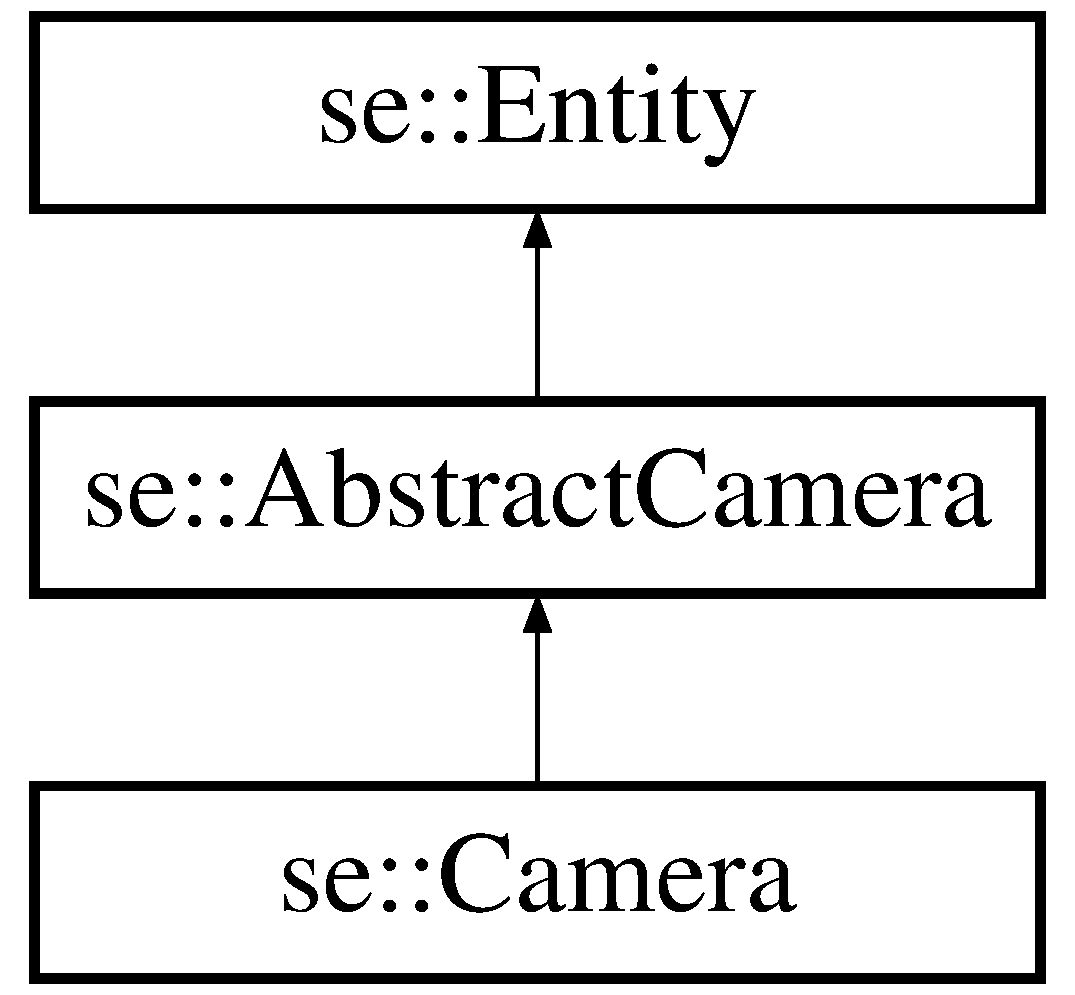
\includegraphics[height=2.000000cm]{classse_1_1_camera}
\end{center}
\end{figure}
\subsection*{Public Member Functions}
\begin{DoxyCompactItemize}
\item 
\mbox{\hyperlink{classse_1_1_camera_a45cc397abfbd7287d96dbbb70330f2e5}{Camera}} (\mbox{\hyperlink{classse_1_1_abstract_renderer}{Abstract\+Renderer}} $\ast$renderer, \mbox{\hyperlink{classse_1_1_abstract_input}{Abstract\+Input}} $\ast$input, const std\+::string \&asset\+Name)
\item 
void \mbox{\hyperlink{classse_1_1_camera_ac49219007d931e1800a33d2603f08856}{Set\+Target}} (\mbox{\hyperlink{namespacese_a12e07512d95e2fdebdaf74a5ea2cf5f6}{Vector3f}} $\ast$position, \mbox{\hyperlink{namespacese_a12e07512d95e2fdebdaf74a5ea2cf5f6}{Vector3f}} $\ast$rotation)
\item 
void \mbox{\hyperlink{classse_1_1_camera_abecf2d50dc793707a475b35bb487812c}{Update}} (float delta) override
\item 
void \mbox{\hyperlink{classse_1_1_camera_accc1f78d52fca1e68c5267fbc0fef239}{Render}} (\mbox{\hyperlink{classse_1_1_abstract_renderer}{Abstract\+Renderer}} $\ast$renderer) override
\item 
\mbox{\hyperlink{namespacese_a12e07512d95e2fdebdaf74a5ea2cf5f6}{Vector3f}} \mbox{\hyperlink{classse_1_1_camera_af3d7f8a74dc26a3840331ab40b6ac893}{Get\+Position}} () const override
\end{DoxyCompactItemize}
\subsection*{Additional Inherited Members}


\subsection{Detailed Description}
A default created camera \mbox{\hyperlink{classse_1_1_entity}{Entity}}. 

Definition at line 13 of file Camera.\+h.



\subsection{Constructor \& Destructor Documentation}
\mbox{\Hypertarget{classse_1_1_camera_a45cc397abfbd7287d96dbbb70330f2e5}\label{classse_1_1_camera_a45cc397abfbd7287d96dbbb70330f2e5}} 
\index{se\+::\+Camera@{se\+::\+Camera}!Camera@{Camera}}
\index{Camera@{Camera}!se\+::\+Camera@{se\+::\+Camera}}
\subsubsection{\texorpdfstring{Camera()}{Camera()}}
{\footnotesize\ttfamily se\+::\+Camera\+::\+Camera (\begin{DoxyParamCaption}\item[{\mbox{\hyperlink{classse_1_1_abstract_renderer}{Abstract\+Renderer}} $\ast$}]{renderer,  }\item[{\mbox{\hyperlink{classse_1_1_abstract_input}{Abstract\+Input}} $\ast$}]{input,  }\item[{const std\+::string \&}]{asset\+Name }\end{DoxyParamCaption})}

Create a camera with a renderer and the input you want to use. 

Definition at line 5 of file Camera.\+cpp.



\subsection{Member Function Documentation}
\mbox{\Hypertarget{classse_1_1_camera_af3d7f8a74dc26a3840331ab40b6ac893}\label{classse_1_1_camera_af3d7f8a74dc26a3840331ab40b6ac893}} 
\index{se\+::\+Camera@{se\+::\+Camera}!Get\+Position@{Get\+Position}}
\index{Get\+Position@{Get\+Position}!se\+::\+Camera@{se\+::\+Camera}}
\subsubsection{\texorpdfstring{Get\+Position()}{GetPosition()}}
{\footnotesize\ttfamily \mbox{\hyperlink{namespacese_a12e07512d95e2fdebdaf74a5ea2cf5f6}{Vector3f}} se\+::\+Camera\+::\+Get\+Position (\begin{DoxyParamCaption}{ }\end{DoxyParamCaption}) const\hspace{0.3cm}{\ttfamily [override]}, {\ttfamily [virtual]}}

Get the current position of the camera. 

Reimplemented from \mbox{\hyperlink{classse_1_1_entity_a40f94e236b724c4e375ee51f923de475}{se\+::\+Entity}}.



Definition at line 86 of file Camera.\+cpp.

\mbox{\Hypertarget{classse_1_1_camera_accc1f78d52fca1e68c5267fbc0fef239}\label{classse_1_1_camera_accc1f78d52fca1e68c5267fbc0fef239}} 
\index{se\+::\+Camera@{se\+::\+Camera}!Render@{Render}}
\index{Render@{Render}!se\+::\+Camera@{se\+::\+Camera}}
\subsubsection{\texorpdfstring{Render()}{Render()}}
{\footnotesize\ttfamily void se\+::\+Camera\+::\+Render (\begin{DoxyParamCaption}\item[{\mbox{\hyperlink{classse_1_1_abstract_renderer}{Abstract\+Renderer}} $\ast$}]{renderer }\end{DoxyParamCaption})\hspace{0.3cm}{\ttfamily [override]}, {\ttfamily [virtual]}}

Render the camera with the asset it is set to, if it\textquotesingle{}s set to anything. 

Implements \mbox{\hyperlink{classse_1_1_entity_a50066f09c64b3b9705b71366cc565527}{se\+::\+Entity}}.



Definition at line 74 of file Camera.\+cpp.

\mbox{\Hypertarget{classse_1_1_camera_ac49219007d931e1800a33d2603f08856}\label{classse_1_1_camera_ac49219007d931e1800a33d2603f08856}} 
\index{se\+::\+Camera@{se\+::\+Camera}!Set\+Target@{Set\+Target}}
\index{Set\+Target@{Set\+Target}!se\+::\+Camera@{se\+::\+Camera}}
\subsubsection{\texorpdfstring{Set\+Target()}{SetTarget()}}
{\footnotesize\ttfamily void se\+::\+Camera\+::\+Set\+Target (\begin{DoxyParamCaption}\item[{\mbox{\hyperlink{namespacese_a12e07512d95e2fdebdaf74a5ea2cf5f6}{Vector3f}} $\ast$}]{position,  }\item[{\mbox{\hyperlink{namespacese_a12e07512d95e2fdebdaf74a5ea2cf5f6}{Vector3f}} $\ast$}]{rotation }\end{DoxyParamCaption})}

Set the position of the camera. 

Definition at line 81 of file Camera.\+cpp.

\mbox{\Hypertarget{classse_1_1_camera_abecf2d50dc793707a475b35bb487812c}\label{classse_1_1_camera_abecf2d50dc793707a475b35bb487812c}} 
\index{se\+::\+Camera@{se\+::\+Camera}!Update@{Update}}
\index{Update@{Update}!se\+::\+Camera@{se\+::\+Camera}}
\subsubsection{\texorpdfstring{Update()}{Update()}}
{\footnotesize\ttfamily void se\+::\+Camera\+::\+Update (\begin{DoxyParamCaption}\item[{float}]{delta }\end{DoxyParamCaption})\hspace{0.3cm}{\ttfamily [override]}, {\ttfamily [virtual]}}

Updates camera logic, it defaults to logic for a freeroaming camera, if a target is set it\textquotesingle{}ll update it to the target. 

Implements \mbox{\hyperlink{classse_1_1_entity_a1542c96865f6646c7b0cb0d9be7f88ad}{se\+::\+Entity}}.



Definition at line 21 of file Camera.\+cpp.



The documentation for this class was generated from the following files\+:\begin{DoxyCompactItemize}
\item 
D\+:/\+Projects/\+Game\+Engine3\+D/\+Include/\mbox{\hyperlink{_camera_8h}{Camera.\+h}}\item 
D\+:/\+Projects/\+Game\+Engine3\+D/\+Source/\mbox{\hyperlink{_camera_8cpp}{Camera.\+cpp}}\end{DoxyCompactItemize}

\hypertarget{classse_1_1_debug}{}\section{se\+:\+:Debug Class Reference}
\label{classse_1_1_debug}\index{se\+::\+Debug@{se\+::\+Debug}}


{\ttfamily \#include $<$Debug.\+h$>$}

\subsection*{Public Member Functions}
\begin{DoxyCompactItemize}
\item 
\mbox{\hyperlink{classse_1_1_debug_a1292de4f720caa545023e0b4a4735eef}{Debug}} (const std\+::string \&path=\char`\"{}default\+\_\+logger.\+log\char`\"{})
\item 
\mbox{\hyperlink{classse_1_1_debug_a2ff6371c83b2a8918b15907bd1491ac9}{$\sim$\+Debug}} ()
\item 
void \mbox{\hyperlink{classse_1_1_debug_a3ebaea1144b70d56762d2b1054c8251d}{Log}} (\mbox{\hyperlink{namespacese_aaa5cbe4d4821d8a349338e23de6ef9c4}{Error\+Type}} error\+Type, const std\+::string \&file, int line, const std\+::string \&message)
\item 
void \mbox{\hyperlink{classse_1_1_debug_ab97d44dca8606c2be2cb709f7e82be09}{Select\+Logger}} (const std\+::string \&path)
\end{DoxyCompactItemize}


\subsection{Detailed Description}
This class writes error messages to files. 

Definition at line 18 of file Debug.\+h.



\subsection{Constructor \& Destructor Documentation}
\mbox{\Hypertarget{classse_1_1_debug_a1292de4f720caa545023e0b4a4735eef}\label{classse_1_1_debug_a1292de4f720caa545023e0b4a4735eef}} 
\index{se\+::\+Debug@{se\+::\+Debug}!Debug@{Debug}}
\index{Debug@{Debug}!se\+::\+Debug@{se\+::\+Debug}}
\subsubsection{\texorpdfstring{Debug()}{Debug()}}
{\footnotesize\ttfamily se\+::\+Debug\+::\+Debug (\begin{DoxyParamCaption}\item[{const std\+::string \&}]{path = {\ttfamily \char`\"{}default\+\_\+logger.log\char`\"{}} }\end{DoxyParamCaption})}

Initialize debug, sets path to a default logger if nothing is given. \mbox{\Hypertarget{classse_1_1_debug_a2ff6371c83b2a8918b15907bd1491ac9}\label{classse_1_1_debug_a2ff6371c83b2a8918b15907bd1491ac9}} 
\index{se\+::\+Debug@{se\+::\+Debug}!````~Debug@{$\sim$\+Debug}}
\index{````~Debug@{$\sim$\+Debug}!se\+::\+Debug@{se\+::\+Debug}}
\subsubsection{\texorpdfstring{$\sim$\+Debug()}{~Debug()}}
{\footnotesize\ttfamily se\+::\+Debug\+::$\sim$\+Debug (\begin{DoxyParamCaption}{ }\end{DoxyParamCaption})}



\subsection{Member Function Documentation}
\mbox{\Hypertarget{classse_1_1_debug_a3ebaea1144b70d56762d2b1054c8251d}\label{classse_1_1_debug_a3ebaea1144b70d56762d2b1054c8251d}} 
\index{se\+::\+Debug@{se\+::\+Debug}!Log@{Log}}
\index{Log@{Log}!se\+::\+Debug@{se\+::\+Debug}}
\subsubsection{\texorpdfstring{Log()}{Log()}}
{\footnotesize\ttfamily void se\+::\+Debug\+::\+Log (\begin{DoxyParamCaption}\item[{\mbox{\hyperlink{namespacese_aaa5cbe4d4821d8a349338e23de6ef9c4}{Error\+Type}}}]{error\+Type,  }\item[{const std\+::string \&}]{file,  }\item[{int}]{line,  }\item[{const std\+::string \&}]{message }\end{DoxyParamCaption})}

Log an error with a warning level (Error\+Type), the file the error is in which is usually given {\bfseries F\+I\+LE}, the line which is usually given {\bfseries L\+I\+NE}, and the message it\textquotesingle{}s supposed to write. \mbox{\Hypertarget{classse_1_1_debug_ab97d44dca8606c2be2cb709f7e82be09}\label{classse_1_1_debug_ab97d44dca8606c2be2cb709f7e82be09}} 
\index{se\+::\+Debug@{se\+::\+Debug}!Select\+Logger@{Select\+Logger}}
\index{Select\+Logger@{Select\+Logger}!se\+::\+Debug@{se\+::\+Debug}}
\subsubsection{\texorpdfstring{Select\+Logger()}{SelectLogger()}}
{\footnotesize\ttfamily void se\+::\+Debug\+::\+Select\+Logger (\begin{DoxyParamCaption}\item[{const std\+::string \&}]{path }\end{DoxyParamCaption})}

Select the file it\textquotesingle{}s supposed to write in. 

The documentation for this class was generated from the following file\+:\begin{DoxyCompactItemize}
\item 
D\+:/\+Projects/\+Game\+Engine3\+D/\+Include/\mbox{\hyperlink{_debug_8h}{Debug.\+h}}\end{DoxyCompactItemize}

\hypertarget{classse_1_1_direct3_d}{}\section{se\+:\+:Direct3D Class Reference}
\label{classse_1_1_direct3_d}\index{se\+::\+Direct3D@{se\+::\+Direct3D}}


{\ttfamily \#include $<$Direct3\+D.\+h$>$}

Inheritance diagram for se\+:\+:Direct3D\+:\begin{figure}[H]
\begin{center}
\leavevmode
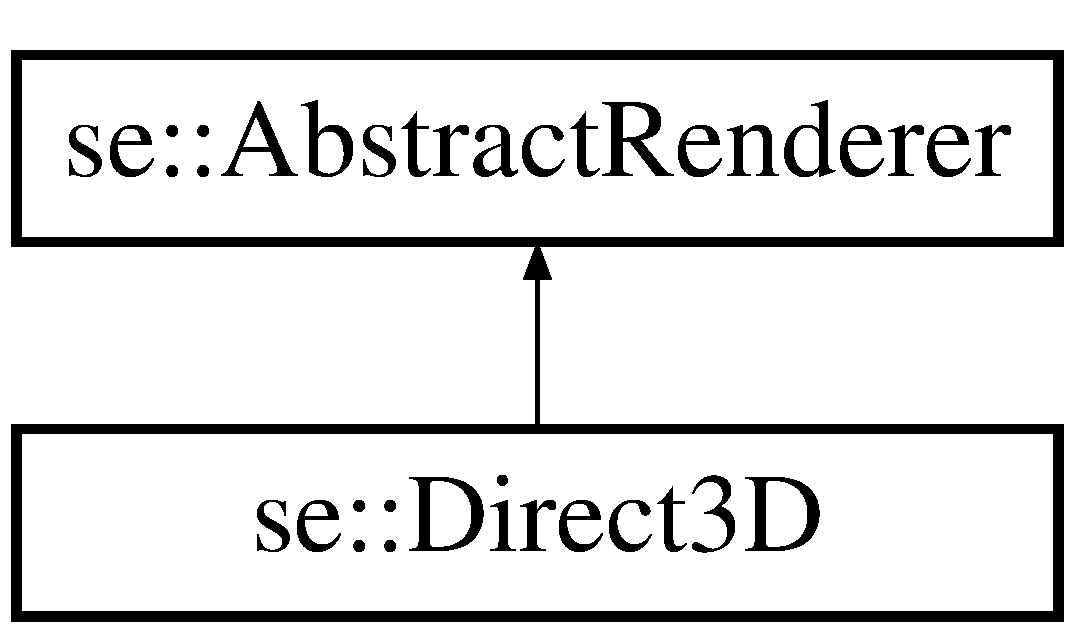
\includegraphics[height=2.000000cm]{classse_1_1_direct3_d}
\end{center}
\end{figure}
\subsection*{Public Member Functions}
\begin{DoxyCompactItemize}
\item 
void \mbox{\hyperlink{classse_1_1_direct3_d_af88b0fb33fe5bff1112213e6c8faf466}{Create}} (int width, int height) override
\item 
void \mbox{\hyperlink{classse_1_1_direct3_d_a39934c194406f108a992d82a4d265381}{Update}} (float delta) override
\item 
void \mbox{\hyperlink{classse_1_1_direct3_d_a31e3c97cd8ceeaea58017b66bd60b9d7}{Render}} (const std\+::string \&buffer\+Name) override
\item 
void \mbox{\hyperlink{classse_1_1_direct3_d_aa87e49a2704cc5da20655ce41ae9782b}{Process}} () override
\item 
void \mbox{\hyperlink{classse_1_1_direct3_d_ae2979f16a5c35773cf2c243d8e6f90e4}{Release}} () override
\item 
void \mbox{\hyperlink{classse_1_1_direct3_d_a77f814cda45f2b490e11c522f8e752e3}{Release}} (const std\+::string \&buffer\+Name) override
\item 
void \mbox{\hyperlink{classse_1_1_direct3_d_a7d5db09c1cf0c5c45f61c631b174fcf2}{Initialize\+Texture\+Array}} (const std\+::string \&buffer\+Name, int size) override
\item 
void \mbox{\hyperlink{classse_1_1_direct3_d_a52e0bbf13e8045dab39bb2ef34028a94}{Create\+Vertex\+Buffer}} (const std\+::string \&buffer\+Name, \mbox{\hyperlink{namespacese_a9ed62241331cac830c5c1ba8450afc2b}{Render\+Type}} type, \mbox{\hyperlink{structse_1_1_vertex}{Vertex}} $\ast$vertices, \mbox{\hyperlink{namespacese_ada11715de7cf6e87b5dfb4611fe68d29}{Vector3i}} $\ast$size=nullptr) override
\item 
void \mbox{\hyperlink{classse_1_1_direct3_d_a33c350a77a959847d3571e14feb72c85}{Create\+Texture}} (const std\+::string \&buffer\+Name, const std\+::string \&path, int id) override
\item 
void \mbox{\hyperlink{classse_1_1_direct3_d_aab3d1a8b4ee8812dea07f5ecda5efc42}{Create\+Mesh}} (const std\+::string \&buffer\+Name, const std\+::string \&path) override
\item 
void \mbox{\hyperlink{classse_1_1_direct3_d_a0294b31c151540af98c78d1e33cb369a}{Set\+View\+Transform}} (\mbox{\hyperlink{namespacese_a12e07512d95e2fdebdaf74a5ea2cf5f6}{Vector3f}} position, \mbox{\hyperlink{namespacese_a12e07512d95e2fdebdaf74a5ea2cf5f6}{Vector3f}} rotation) override
\item 
\mbox{\hyperlink{namespacese_a12e07512d95e2fdebdaf74a5ea2cf5f6}{Vector3f}} \mbox{\hyperlink{classse_1_1_direct3_d_a74d6926ba18dac6ce23c7dea433de7bd}{Get\+View\+Axes}} () override
\end{DoxyCompactItemize}


\subsection{Detailed Description}
The renderer for DirectX 9. 

Definition at line 28 of file Direct3\+D.\+h.



\subsection{Member Function Documentation}
\mbox{\Hypertarget{classse_1_1_direct3_d_af88b0fb33fe5bff1112213e6c8faf466}\label{classse_1_1_direct3_d_af88b0fb33fe5bff1112213e6c8faf466}} 
\index{se\+::\+Direct3D@{se\+::\+Direct3D}!Create@{Create}}
\index{Create@{Create}!se\+::\+Direct3D@{se\+::\+Direct3D}}
\subsubsection{\texorpdfstring{Create()}{Create()}}
{\footnotesize\ttfamily void se\+::\+Direct3\+D\+::\+Create (\begin{DoxyParamCaption}\item[{int}]{width,  }\item[{int}]{height }\end{DoxyParamCaption})\hspace{0.3cm}{\ttfamily [override]}, {\ttfamily [virtual]}}

Creates a DirectX renderer for the latest created \mbox{\hyperlink{classse_1_1_window}{Window}} in \mbox{\hyperlink{classse_1_1_window_manager}{Window\+Manager}}, it creates a new Swap\+Chain and adds it to the list. 

Implements \mbox{\hyperlink{classse_1_1_abstract_renderer_a3b0c7d8dc34c56513b3160e2cf1e094a}{se\+::\+Abstract\+Renderer}}.

\mbox{\Hypertarget{classse_1_1_direct3_d_aab3d1a8b4ee8812dea07f5ecda5efc42}\label{classse_1_1_direct3_d_aab3d1a8b4ee8812dea07f5ecda5efc42}} 
\index{se\+::\+Direct3D@{se\+::\+Direct3D}!Create\+Mesh@{Create\+Mesh}}
\index{Create\+Mesh@{Create\+Mesh}!se\+::\+Direct3D@{se\+::\+Direct3D}}
\subsubsection{\texorpdfstring{Create\+Mesh()}{CreateMesh()}}
{\footnotesize\ttfamily void se\+::\+Direct3\+D\+::\+Create\+Mesh (\begin{DoxyParamCaption}\item[{const std\+::string \&}]{buffer\+Name,  }\item[{const std\+::string \&}]{path }\end{DoxyParamCaption})\hspace{0.3cm}{\ttfamily [override]}, {\ttfamily [virtual]}}

Create a mesh with an .x file with the Direct\+X9 default pipeline to a given buffer. 

Implements \mbox{\hyperlink{classse_1_1_abstract_renderer_a4a3e8836f7a8b1b35a5f7cb1b4231476}{se\+::\+Abstract\+Renderer}}.

\mbox{\Hypertarget{classse_1_1_direct3_d_a33c350a77a959847d3571e14feb72c85}\label{classse_1_1_direct3_d_a33c350a77a959847d3571e14feb72c85}} 
\index{se\+::\+Direct3D@{se\+::\+Direct3D}!Create\+Texture@{Create\+Texture}}
\index{Create\+Texture@{Create\+Texture}!se\+::\+Direct3D@{se\+::\+Direct3D}}
\subsubsection{\texorpdfstring{Create\+Texture()}{CreateTexture()}}
{\footnotesize\ttfamily void se\+::\+Direct3\+D\+::\+Create\+Texture (\begin{DoxyParamCaption}\item[{const std\+::string \&}]{buffer\+Name,  }\item[{const std\+::string \&}]{path,  }\item[{int}]{id }\end{DoxyParamCaption})\hspace{0.3cm}{\ttfamily [override]}, {\ttfamily [virtual]}}

To create a texture the texture array needs to be initialized with Initialize\+Texture\+Array to a given buffer. 

Implements \mbox{\hyperlink{classse_1_1_abstract_renderer_a89f2efd2ee68cfb6735e51ce87206dfd}{se\+::\+Abstract\+Renderer}}.

\mbox{\Hypertarget{classse_1_1_direct3_d_a52e0bbf13e8045dab39bb2ef34028a94}\label{classse_1_1_direct3_d_a52e0bbf13e8045dab39bb2ef34028a94}} 
\index{se\+::\+Direct3D@{se\+::\+Direct3D}!Create\+Vertex\+Buffer@{Create\+Vertex\+Buffer}}
\index{Create\+Vertex\+Buffer@{Create\+Vertex\+Buffer}!se\+::\+Direct3D@{se\+::\+Direct3D}}
\subsubsection{\texorpdfstring{Create\+Vertex\+Buffer()}{CreateVertexBuffer()}}
{\footnotesize\ttfamily void se\+::\+Direct3\+D\+::\+Create\+Vertex\+Buffer (\begin{DoxyParamCaption}\item[{const std\+::string \&}]{buffer\+Name,  }\item[{\mbox{\hyperlink{namespacese_a9ed62241331cac830c5c1ba8450afc2b}{Render\+Type}}}]{type,  }\item[{\mbox{\hyperlink{structse_1_1_vertex}{Vertex}} $\ast$}]{vertices,  }\item[{\mbox{\hyperlink{namespacese_ada11715de7cf6e87b5dfb4611fe68d29}{Vector3i}} $\ast$}]{size = {\ttfamily nullptr} }\end{DoxyParamCaption})\hspace{0.3cm}{\ttfamily [override]}, {\ttfamily [virtual]}}

Create a vertex buffer for a specific Render\+Type with the referenced vertices array and size for the primitivecount. 

Implements \mbox{\hyperlink{classse_1_1_abstract_renderer_a953d57d04771acae78c3725bee3639d4}{se\+::\+Abstract\+Renderer}}.

\mbox{\Hypertarget{classse_1_1_direct3_d_a74d6926ba18dac6ce23c7dea433de7bd}\label{classse_1_1_direct3_d_a74d6926ba18dac6ce23c7dea433de7bd}} 
\index{se\+::\+Direct3D@{se\+::\+Direct3D}!Get\+View\+Axes@{Get\+View\+Axes}}
\index{Get\+View\+Axes@{Get\+View\+Axes}!se\+::\+Direct3D@{se\+::\+Direct3D}}
\subsubsection{\texorpdfstring{Get\+View\+Axes()}{GetViewAxes()}}
{\footnotesize\ttfamily \mbox{\hyperlink{namespacese_a12e07512d95e2fdebdaf74a5ea2cf5f6}{Vector3f}} se\+::\+Direct3\+D\+::\+Get\+View\+Axes (\begin{DoxyParamCaption}{ }\end{DoxyParamCaption})\hspace{0.3cm}{\ttfamily [override]}, {\ttfamily [virtual]}}

Get the current axes of the view. 

Implements \mbox{\hyperlink{classse_1_1_abstract_renderer_a8af4c1bef5cf120f6160f5d93dd74207}{se\+::\+Abstract\+Renderer}}.

\mbox{\Hypertarget{classse_1_1_direct3_d_a7d5db09c1cf0c5c45f61c631b174fcf2}\label{classse_1_1_direct3_d_a7d5db09c1cf0c5c45f61c631b174fcf2}} 
\index{se\+::\+Direct3D@{se\+::\+Direct3D}!Initialize\+Texture\+Array@{Initialize\+Texture\+Array}}
\index{Initialize\+Texture\+Array@{Initialize\+Texture\+Array}!se\+::\+Direct3D@{se\+::\+Direct3D}}
\subsubsection{\texorpdfstring{Initialize\+Texture\+Array()}{InitializeTextureArray()}}
{\footnotesize\ttfamily void se\+::\+Direct3\+D\+::\+Initialize\+Texture\+Array (\begin{DoxyParamCaption}\item[{const std\+::string \&}]{buffer\+Name,  }\item[{int}]{size }\end{DoxyParamCaption})\hspace{0.3cm}{\ttfamily [override]}, {\ttfamily [virtual]}}

Initialize a texture array to create texture(s) within that list to a given buffer. 

Implements \mbox{\hyperlink{classse_1_1_abstract_renderer_afd7697df1d4958ec3b0fa13109a269a1}{se\+::\+Abstract\+Renderer}}.

\mbox{\Hypertarget{classse_1_1_direct3_d_aa87e49a2704cc5da20655ce41ae9782b}\label{classse_1_1_direct3_d_aa87e49a2704cc5da20655ce41ae9782b}} 
\index{se\+::\+Direct3D@{se\+::\+Direct3D}!Process@{Process}}
\index{Process@{Process}!se\+::\+Direct3D@{se\+::\+Direct3D}}
\subsubsection{\texorpdfstring{Process()}{Process()}}
{\footnotesize\ttfamily void se\+::\+Direct3\+D\+::\+Process (\begin{DoxyParamCaption}{ }\end{DoxyParamCaption})\hspace{0.3cm}{\ttfamily [override]}, {\ttfamily [virtual]}}

Here it loops through all the windows, clears the screen, sets the backbuffer and begins, ends and presents the scene. It also sets the scale, rotation and position of all the entities of the current scene. 

Implements \mbox{\hyperlink{classse_1_1_abstract_renderer_a90596b2d067b4fa197b809191407be97}{se\+::\+Abstract\+Renderer}}.

\mbox{\Hypertarget{classse_1_1_direct3_d_ae2979f16a5c35773cf2c243d8e6f90e4}\label{classse_1_1_direct3_d_ae2979f16a5c35773cf2c243d8e6f90e4}} 
\index{se\+::\+Direct3D@{se\+::\+Direct3D}!Release@{Release}}
\index{Release@{Release}!se\+::\+Direct3D@{se\+::\+Direct3D}}
\subsubsection{\texorpdfstring{Release()}{Release()}\hspace{0.1cm}{\footnotesize\ttfamily [1/2]}}
{\footnotesize\ttfamily void se\+::\+Direct3\+D\+::\+Release (\begin{DoxyParamCaption}{ }\end{DoxyParamCaption})\hspace{0.3cm}{\ttfamily [override]}, {\ttfamily [virtual]}}

Release all the swapchains, the device and direct3d. 

Implements \mbox{\hyperlink{classse_1_1_abstract_renderer_a98e35b7db62827580573185ed91b25bb}{se\+::\+Abstract\+Renderer}}.

\mbox{\Hypertarget{classse_1_1_direct3_d_a77f814cda45f2b490e11c522f8e752e3}\label{classse_1_1_direct3_d_a77f814cda45f2b490e11c522f8e752e3}} 
\index{se\+::\+Direct3D@{se\+::\+Direct3D}!Release@{Release}}
\index{Release@{Release}!se\+::\+Direct3D@{se\+::\+Direct3D}}
\subsubsection{\texorpdfstring{Release()}{Release()}\hspace{0.1cm}{\footnotesize\ttfamily [2/2]}}
{\footnotesize\ttfamily void se\+::\+Direct3\+D\+::\+Release (\begin{DoxyParamCaption}\item[{const std\+::string \&}]{buffer\+Name }\end{DoxyParamCaption})\hspace{0.3cm}{\ttfamily [override]}, {\ttfamily [virtual]}}

Release all components of a single \mbox{\hyperlink{structse_1_1_draw_components}{Draw\+Components}} with the buffername in the componentslist. 

Implements \mbox{\hyperlink{classse_1_1_abstract_renderer_af6d6d012f070f95d4c49713002872fcc}{se\+::\+Abstract\+Renderer}}.

\mbox{\Hypertarget{classse_1_1_direct3_d_a31e3c97cd8ceeaea58017b66bd60b9d7}\label{classse_1_1_direct3_d_a31e3c97cd8ceeaea58017b66bd60b9d7}} 
\index{se\+::\+Direct3D@{se\+::\+Direct3D}!Render@{Render}}
\index{Render@{Render}!se\+::\+Direct3D@{se\+::\+Direct3D}}
\subsubsection{\texorpdfstring{Render()}{Render()}}
{\footnotesize\ttfamily void se\+::\+Direct3\+D\+::\+Render (\begin{DoxyParamCaption}\item[{const std\+::string \&}]{buffer\+Name }\end{DoxyParamCaption})\hspace{0.3cm}{\ttfamily [override]}, {\ttfamily [virtual]}}

It sets all the relevant settings for the components and then draws the component. 

Implements \mbox{\hyperlink{classse_1_1_abstract_renderer_a76058a91574874ab3c51294a2c9ea85c}{se\+::\+Abstract\+Renderer}}.

\mbox{\Hypertarget{classse_1_1_direct3_d_a0294b31c151540af98c78d1e33cb369a}\label{classse_1_1_direct3_d_a0294b31c151540af98c78d1e33cb369a}} 
\index{se\+::\+Direct3D@{se\+::\+Direct3D}!Set\+View\+Transform@{Set\+View\+Transform}}
\index{Set\+View\+Transform@{Set\+View\+Transform}!se\+::\+Direct3D@{se\+::\+Direct3D}}
\subsubsection{\texorpdfstring{Set\+View\+Transform()}{SetViewTransform()}}
{\footnotesize\ttfamily void se\+::\+Direct3\+D\+::\+Set\+View\+Transform (\begin{DoxyParamCaption}\item[{\mbox{\hyperlink{namespacese_a12e07512d95e2fdebdaf74a5ea2cf5f6}{Vector3f}}}]{position,  }\item[{\mbox{\hyperlink{namespacese_a12e07512d95e2fdebdaf74a5ea2cf5f6}{Vector3f}}}]{rotation }\end{DoxyParamCaption})\hspace{0.3cm}{\ttfamily [override]}, {\ttfamily [virtual]}}

Set the position and rotation for the screen view. 

Implements \mbox{\hyperlink{classse_1_1_abstract_renderer_a710e67232e977fbb3b74f79640e0b62e}{se\+::\+Abstract\+Renderer}}.

\mbox{\Hypertarget{classse_1_1_direct3_d_a39934c194406f108a992d82a4d265381}\label{classse_1_1_direct3_d_a39934c194406f108a992d82a4d265381}} 
\index{se\+::\+Direct3D@{se\+::\+Direct3D}!Update@{Update}}
\index{Update@{Update}!se\+::\+Direct3D@{se\+::\+Direct3D}}
\subsubsection{\texorpdfstring{Update()}{Update()}}
{\footnotesize\ttfamily void se\+::\+Direct3\+D\+::\+Update (\begin{DoxyParamCaption}\item[{float}]{delta }\end{DoxyParamCaption})\hspace{0.3cm}{\ttfamily [override]}, {\ttfamily [virtual]}}

Updates the view for the latest added camera. 

Implements \mbox{\hyperlink{classse_1_1_abstract_renderer_aae49e7417663d6a5aca34a2bb37b4b28}{se\+::\+Abstract\+Renderer}}.



The documentation for this class was generated from the following file\+:\begin{DoxyCompactItemize}
\item 
D\+:/\+Projects/\+Game\+Engine3\+D/\+Include/\+Direct\+X9/\mbox{\hyperlink{_direct3_d_8h}{Direct3\+D.\+h}}\end{DoxyCompactItemize}

\hypertarget{classse_1_1_direct_input}{}\section{se\+:\+:Direct\+Input Class Reference}
\label{classse_1_1_direct_input}\index{se\+::\+Direct\+Input@{se\+::\+Direct\+Input}}


{\ttfamily \#include $<$Direct\+Input.\+h$>$}

Inheritance diagram for se\+:\+:Direct\+Input\+:\begin{figure}[H]
\begin{center}
\leavevmode
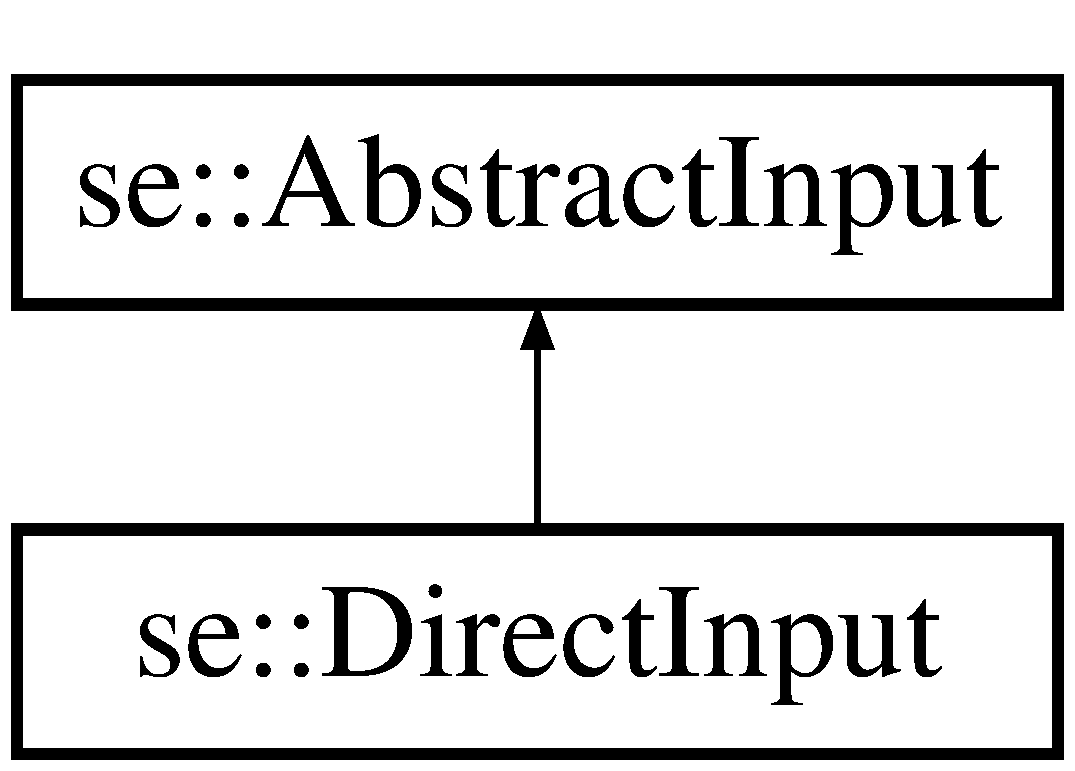
\includegraphics[height=2.000000cm]{classse_1_1_direct_input}
\end{center}
\end{figure}
\subsection*{Public Member Functions}
\begin{DoxyCompactItemize}
\item 
\mbox{\hyperlink{classse_1_1_direct_input_a2e5e8da67102c194b874fdfa04ca40e4}{Direct\+Input}} ()
\item 
\mbox{\hyperlink{classse_1_1_direct_input_a5ff50cb2afc8d67116856c34169429d0}{$\sim$\+Direct\+Input}} ()
\item 
bool \mbox{\hyperlink{classse_1_1_direct_input_ae8f8c4306ad58f7696548d2c63f01e6f}{Initialize}} (H\+I\+N\+S\+T\+A\+N\+CE h\+Instance, H\+W\+ND h\+Wnd, int screen\+Width, int screen\+Height) override
\item 
bool \mbox{\hyperlink{classse_1_1_direct_input_ad9669e6834c3fcac489050a82beb71f7}{Is\+Pressed}} (\mbox{\hyperlink{namespacese_a94221cf8f238f1eadbe3ac4b8ac7bc71}{Keyboard\+Key}} key) override
\item 
void \mbox{\hyperlink{classse_1_1_direct_input_a863123d7304364a55fd2135f27195500}{Update}} () override
\item 
void \mbox{\hyperlink{classse_1_1_direct_input_a3c097a463a36421a13bf05819c4b681e}{Get\+Mouse\+Location}} (int \&mouseX, int \&mouseY) override
\end{DoxyCompactItemize}


\subsection{Detailed Description}
You can use this class to handle input with Direct\+X9. 

Definition at line 14 of file Direct\+Input.\+h.



\subsection{Constructor \& Destructor Documentation}
\mbox{\Hypertarget{classse_1_1_direct_input_a2e5e8da67102c194b874fdfa04ca40e4}\label{classse_1_1_direct_input_a2e5e8da67102c194b874fdfa04ca40e4}} 
\index{se\+::\+Direct\+Input@{se\+::\+Direct\+Input}!Direct\+Input@{Direct\+Input}}
\index{Direct\+Input@{Direct\+Input}!se\+::\+Direct\+Input@{se\+::\+Direct\+Input}}
\subsubsection{\texorpdfstring{Direct\+Input()}{DirectInput()}}
{\footnotesize\ttfamily se\+::\+Direct\+Input\+::\+Direct\+Input (\begin{DoxyParamCaption}{ }\end{DoxyParamCaption})}



Definition at line 5 of file Direct\+Input.\+cpp.

\mbox{\Hypertarget{classse_1_1_direct_input_a5ff50cb2afc8d67116856c34169429d0}\label{classse_1_1_direct_input_a5ff50cb2afc8d67116856c34169429d0}} 
\index{se\+::\+Direct\+Input@{se\+::\+Direct\+Input}!````~Direct\+Input@{$\sim$\+Direct\+Input}}
\index{````~Direct\+Input@{$\sim$\+Direct\+Input}!se\+::\+Direct\+Input@{se\+::\+Direct\+Input}}
\subsubsection{\texorpdfstring{$\sim$\+Direct\+Input()}{~DirectInput()}}
{\footnotesize\ttfamily se\+::\+Direct\+Input\+::$\sim$\+Direct\+Input (\begin{DoxyParamCaption}{ }\end{DoxyParamCaption})}



Definition at line 12 of file Direct\+Input.\+cpp.



\subsection{Member Function Documentation}
\mbox{\Hypertarget{classse_1_1_direct_input_a3c097a463a36421a13bf05819c4b681e}\label{classse_1_1_direct_input_a3c097a463a36421a13bf05819c4b681e}} 
\index{se\+::\+Direct\+Input@{se\+::\+Direct\+Input}!Get\+Mouse\+Location@{Get\+Mouse\+Location}}
\index{Get\+Mouse\+Location@{Get\+Mouse\+Location}!se\+::\+Direct\+Input@{se\+::\+Direct\+Input}}
\subsubsection{\texorpdfstring{Get\+Mouse\+Location()}{GetMouseLocation()}}
{\footnotesize\ttfamily void se\+::\+Direct\+Input\+::\+Get\+Mouse\+Location (\begin{DoxyParamCaption}\item[{int \&}]{mouseX,  }\item[{int \&}]{mouseY }\end{DoxyParamCaption})\hspace{0.3cm}{\ttfamily [override]}, {\ttfamily [virtual]}}

Get the mouse location. 

Implements \mbox{\hyperlink{classse_1_1_abstract_input_a93673fb3534be8bbc1f495f650064b91}{se\+::\+Abstract\+Input}}.



Definition at line 148 of file Direct\+Input.\+cpp.

\mbox{\Hypertarget{classse_1_1_direct_input_ae8f8c4306ad58f7696548d2c63f01e6f}\label{classse_1_1_direct_input_ae8f8c4306ad58f7696548d2c63f01e6f}} 
\index{se\+::\+Direct\+Input@{se\+::\+Direct\+Input}!Initialize@{Initialize}}
\index{Initialize@{Initialize}!se\+::\+Direct\+Input@{se\+::\+Direct\+Input}}
\subsubsection{\texorpdfstring{Initialize()}{Initialize()}}
{\footnotesize\ttfamily bool se\+::\+Direct\+Input\+::\+Initialize (\begin{DoxyParamCaption}\item[{H\+I\+N\+S\+T\+A\+N\+CE}]{h\+Instance,  }\item[{H\+W\+ND}]{h\+Wnd,  }\item[{int}]{screen\+Width,  }\item[{int}]{screen\+Height }\end{DoxyParamCaption})\hspace{0.3cm}{\ttfamily [override]}, {\ttfamily [virtual]}}

Initialize the input for the given window instance and handle. 

Implements \mbox{\hyperlink{classse_1_1_abstract_input_a6219cdd66247d08f3ca52b2fea305b8d}{se\+::\+Abstract\+Input}}.



Definition at line 29 of file Direct\+Input.\+cpp.

\mbox{\Hypertarget{classse_1_1_direct_input_ad9669e6834c3fcac489050a82beb71f7}\label{classse_1_1_direct_input_ad9669e6834c3fcac489050a82beb71f7}} 
\index{se\+::\+Direct\+Input@{se\+::\+Direct\+Input}!Is\+Pressed@{Is\+Pressed}}
\index{Is\+Pressed@{Is\+Pressed}!se\+::\+Direct\+Input@{se\+::\+Direct\+Input}}
\subsubsection{\texorpdfstring{Is\+Pressed()}{IsPressed()}}
{\footnotesize\ttfamily bool se\+::\+Direct\+Input\+::\+Is\+Pressed (\begin{DoxyParamCaption}\item[{\mbox{\hyperlink{namespacese_a94221cf8f238f1eadbe3ac4b8ac7bc71}{Keyboard\+Key}}}]{key }\end{DoxyParamCaption})\hspace{0.3cm}{\ttfamily [override]}, {\ttfamily [virtual]}}

Check if specified Keyboard\+Key is pressed. 

Implements \mbox{\hyperlink{classse_1_1_abstract_input_a4375b92281cee63064c898a791ddd1a3}{se\+::\+Abstract\+Input}}.



Definition at line 129 of file Direct\+Input.\+cpp.

\mbox{\Hypertarget{classse_1_1_direct_input_a863123d7304364a55fd2135f27195500}\label{classse_1_1_direct_input_a863123d7304364a55fd2135f27195500}} 
\index{se\+::\+Direct\+Input@{se\+::\+Direct\+Input}!Update@{Update}}
\index{Update@{Update}!se\+::\+Direct\+Input@{se\+::\+Direct\+Input}}
\subsubsection{\texorpdfstring{Update()}{Update()}}
{\footnotesize\ttfamily void se\+::\+Direct\+Input\+::\+Update (\begin{DoxyParamCaption}{ }\end{DoxyParamCaption})\hspace{0.3cm}{\ttfamily [override]}, {\ttfamily [virtual]}}

Update the read key/mouse input. 

Implements \mbox{\hyperlink{classse_1_1_abstract_input_a7c9b63e9df453d38c035fb9fa91c0d70}{se\+::\+Abstract\+Input}}.



Definition at line 105 of file Direct\+Input.\+cpp.



The documentation for this class was generated from the following files\+:\begin{DoxyCompactItemize}
\item 
D\+:/\+Projects/\+Game\+Engine3\+D/\+Include/\+Direct\+X9/\mbox{\hyperlink{_direct_input_8h}{Direct\+Input.\+h}}\item 
D\+:/\+Projects/\+Game\+Engine3\+D/\+Source/\+Direct\+X9/\mbox{\hyperlink{_direct_input_8cpp}{Direct\+Input.\+cpp}}\end{DoxyCompactItemize}

\hypertarget{structse_1_1_draw_components}{}\section{se\+:\+:Draw\+Components Struct Reference}
\label{structse_1_1_draw_components}\index{se\+::\+Draw\+Components@{se\+::\+Draw\+Components}}


{\ttfamily \#include $<$Direct3\+D.\+h$>$}

\subsection*{Public Attributes}
\begin{DoxyCompactItemize}
\item 
D3\+D\+M\+A\+T\+E\+R\+I\+A\+L9 $\ast$ \mbox{\hyperlink{structse_1_1_draw_components_a6e72bd7d854097cd4371c8b5dbdaed87}{materials}}
\item 
L\+P\+D3\+D\+X\+M\+E\+SH \mbox{\hyperlink{structse_1_1_draw_components_ad8dbb551cea22f21b227cb37e4b43f95}{mesh}} = nullptr
\item 
L\+P\+D\+I\+R\+E\+C\+T3\+D\+V\+E\+R\+T\+E\+X\+B\+U\+F\+F\+E\+R9 \mbox{\hyperlink{structse_1_1_draw_components_ab98ae9279575ab342380577a2a1d83d1}{buffer}}
\item 
L\+P\+D\+I\+R\+E\+C\+T3\+D\+T\+E\+X\+T\+U\+R\+E9 $\ast$ \mbox{\hyperlink{structse_1_1_draw_components_a5853cbdf5f707c4cd3cffb09678cfe18}{textures}}
\item 
int \mbox{\hyperlink{structse_1_1_draw_components_af74ab24e473de232a1df0166109cbafd}{primitive\+Count}} = 0
\item 
int \mbox{\hyperlink{structse_1_1_draw_components_a4a4323bb918073fe2c6cf45ee3c885d2}{texture\+Count}} = 0
\item 
bool \mbox{\hyperlink{structse_1_1_draw_components_af32638734af65bd440b7776a7e1694e0}{mip\+Map}} = false
\end{DoxyCompactItemize}


\subsection{Detailed Description}
A structure for getting relevant components. 

Definition at line 15 of file Direct3\+D.\+h.



\subsection{Member Data Documentation}
\mbox{\Hypertarget{structse_1_1_draw_components_ab98ae9279575ab342380577a2a1d83d1}\label{structse_1_1_draw_components_ab98ae9279575ab342380577a2a1d83d1}} 
\index{se\+::\+Draw\+Components@{se\+::\+Draw\+Components}!buffer@{buffer}}
\index{buffer@{buffer}!se\+::\+Draw\+Components@{se\+::\+Draw\+Components}}
\subsubsection{\texorpdfstring{buffer}{buffer}}
{\footnotesize\ttfamily L\+P\+D\+I\+R\+E\+C\+T3\+D\+V\+E\+R\+T\+E\+X\+B\+U\+F\+F\+E\+R9 se\+::\+Draw\+Components\+::buffer}



Definition at line 18 of file Direct3\+D.\+h.

\mbox{\Hypertarget{structse_1_1_draw_components_a6e72bd7d854097cd4371c8b5dbdaed87}\label{structse_1_1_draw_components_a6e72bd7d854097cd4371c8b5dbdaed87}} 
\index{se\+::\+Draw\+Components@{se\+::\+Draw\+Components}!materials@{materials}}
\index{materials@{materials}!se\+::\+Draw\+Components@{se\+::\+Draw\+Components}}
\subsubsection{\texorpdfstring{materials}{materials}}
{\footnotesize\ttfamily D3\+D\+M\+A\+T\+E\+R\+I\+A\+L9$\ast$ se\+::\+Draw\+Components\+::materials}



Definition at line 16 of file Direct3\+D.\+h.

\mbox{\Hypertarget{structse_1_1_draw_components_ad8dbb551cea22f21b227cb37e4b43f95}\label{structse_1_1_draw_components_ad8dbb551cea22f21b227cb37e4b43f95}} 
\index{se\+::\+Draw\+Components@{se\+::\+Draw\+Components}!mesh@{mesh}}
\index{mesh@{mesh}!se\+::\+Draw\+Components@{se\+::\+Draw\+Components}}
\subsubsection{\texorpdfstring{mesh}{mesh}}
{\footnotesize\ttfamily L\+P\+D3\+D\+X\+M\+E\+SH se\+::\+Draw\+Components\+::mesh = nullptr}



Definition at line 17 of file Direct3\+D.\+h.

\mbox{\Hypertarget{structse_1_1_draw_components_af32638734af65bd440b7776a7e1694e0}\label{structse_1_1_draw_components_af32638734af65bd440b7776a7e1694e0}} 
\index{se\+::\+Draw\+Components@{se\+::\+Draw\+Components}!mip\+Map@{mip\+Map}}
\index{mip\+Map@{mip\+Map}!se\+::\+Draw\+Components@{se\+::\+Draw\+Components}}
\subsubsection{\texorpdfstring{mip\+Map}{mipMap}}
{\footnotesize\ttfamily bool se\+::\+Draw\+Components\+::mip\+Map = false}



Definition at line 22 of file Direct3\+D.\+h.

\mbox{\Hypertarget{structse_1_1_draw_components_af74ab24e473de232a1df0166109cbafd}\label{structse_1_1_draw_components_af74ab24e473de232a1df0166109cbafd}} 
\index{se\+::\+Draw\+Components@{se\+::\+Draw\+Components}!primitive\+Count@{primitive\+Count}}
\index{primitive\+Count@{primitive\+Count}!se\+::\+Draw\+Components@{se\+::\+Draw\+Components}}
\subsubsection{\texorpdfstring{primitive\+Count}{primitiveCount}}
{\footnotesize\ttfamily int se\+::\+Draw\+Components\+::primitive\+Count = 0}



Definition at line 20 of file Direct3\+D.\+h.

\mbox{\Hypertarget{structse_1_1_draw_components_a4a4323bb918073fe2c6cf45ee3c885d2}\label{structse_1_1_draw_components_a4a4323bb918073fe2c6cf45ee3c885d2}} 
\index{se\+::\+Draw\+Components@{se\+::\+Draw\+Components}!texture\+Count@{texture\+Count}}
\index{texture\+Count@{texture\+Count}!se\+::\+Draw\+Components@{se\+::\+Draw\+Components}}
\subsubsection{\texorpdfstring{texture\+Count}{textureCount}}
{\footnotesize\ttfamily int se\+::\+Draw\+Components\+::texture\+Count = 0}



Definition at line 21 of file Direct3\+D.\+h.

\mbox{\Hypertarget{structse_1_1_draw_components_a5853cbdf5f707c4cd3cffb09678cfe18}\label{structse_1_1_draw_components_a5853cbdf5f707c4cd3cffb09678cfe18}} 
\index{se\+::\+Draw\+Components@{se\+::\+Draw\+Components}!textures@{textures}}
\index{textures@{textures}!se\+::\+Draw\+Components@{se\+::\+Draw\+Components}}
\subsubsection{\texorpdfstring{textures}{textures}}
{\footnotesize\ttfamily L\+P\+D\+I\+R\+E\+C\+T3\+D\+T\+E\+X\+T\+U\+R\+E9$\ast$ se\+::\+Draw\+Components\+::textures}



Definition at line 19 of file Direct3\+D.\+h.



The documentation for this struct was generated from the following file\+:\begin{DoxyCompactItemize}
\item 
D\+:/\+Projects/\+Game\+Engine3\+D/\+Include/\+Direct\+X9/\mbox{\hyperlink{_direct3_d_8h}{Direct3\+D.\+h}}\end{DoxyCompactItemize}

\hypertarget{classse_1_1_entity}{}\section{se\+:\+:Entity Class Reference}
\label{classse_1_1_entity}\index{se\+::\+Entity@{se\+::\+Entity}}


{\ttfamily \#include $<$Entity.\+h$>$}

Inheritance diagram for se\+:\+:Entity\+:\begin{figure}[H]
\begin{center}
\leavevmode
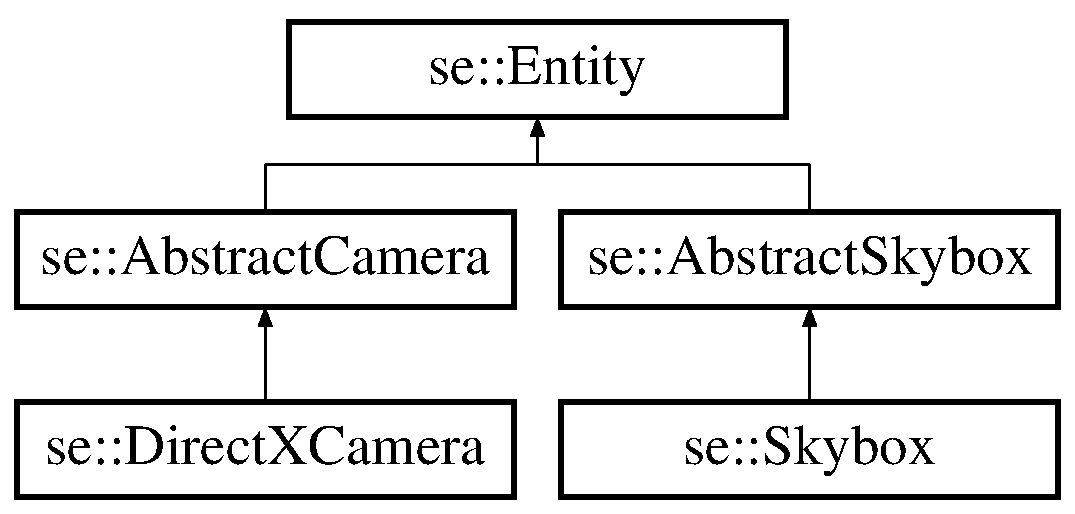
\includegraphics[height=2.000000cm]{classse_1_1_entity}
\end{center}
\end{figure}
\subsection*{Public Member Functions}
\begin{DoxyCompactItemize}
\item 
\mbox{\hyperlink{classse_1_1_entity_ac92492302d50c22ba7c4e9ff016b6145}{Entity}} ()
\item 
void \mbox{\hyperlink{classse_1_1_entity_a09e198e70620f231106d9f375f7598f3}{Set\+Position}} (float x, float y, float z)
\item 
void \mbox{\hyperlink{classse_1_1_entity_ae0d37a4774afab2b7abf4118efc57499}{Set\+Position}} (\mbox{\hyperlink{namespacese_a12e07512d95e2fdebdaf74a5ea2cf5f6}{Vector3f}} position)
\item 
void \mbox{\hyperlink{classse_1_1_entity_a812b63adcbf5f1a3e429a31c6e0ff940}{Set\+Scale}} (float x, float y, float z)
\item 
void \mbox{\hyperlink{classse_1_1_entity_a70df7cdf2d72ff4d767033c2994b673f}{Set\+Scale}} (\mbox{\hyperlink{namespacese_a12e07512d95e2fdebdaf74a5ea2cf5f6}{Vector3f}} scale)
\item 
void \mbox{\hyperlink{classse_1_1_entity_a41f820b99b2b6d76c97472dcddca7fa2}{Set\+Rotation}} (float x, float y, float z)
\item 
void \mbox{\hyperlink{classse_1_1_entity_a950373cfaaad7ad4bba06f3ab8534efd}{Set\+Rotation}} (\mbox{\hyperlink{namespacese_a12e07512d95e2fdebdaf74a5ea2cf5f6}{Vector3f}} rotation)
\item 
void \mbox{\hyperlink{classse_1_1_entity_a4fcf5639a2e6e74e0b12893e70a46a83}{Set\+Asset\+Name}} (const std\+::string \&asset\+Name)
\item 
void \mbox{\hyperlink{classse_1_1_entity_a0550faa593742dbd41284971c24c410e}{Set\+Entity\+Type}} (\mbox{\hyperlink{namespacese_ae73a909a94998bc95235eb9b16e405f1}{Entity\+Type}} type)
\item 
std\+::string \mbox{\hyperlink{classse_1_1_entity_af1d512cba984ffe167decd7ecf7a88f4}{Get\+Asset\+Name}} () const
\item 
\mbox{\hyperlink{namespacese_ae73a909a94998bc95235eb9b16e405f1}{Entity\+Type}} \mbox{\hyperlink{classse_1_1_entity_aec26e9fd7f7c4c6d89e1e459a5eb028a}{Get\+Entity\+Type}} () const
\item 
virtual void \mbox{\hyperlink{classse_1_1_entity_a1cd277c4c5a517f5cde8b72d5c40a8f0}{Update}} (float delta)
\item 
virtual void \mbox{\hyperlink{classse_1_1_entity_aac1c64a40d796cfda308aaa88214bf1c}{Release}} ()
\item 
\mbox{\hyperlink{namespacese_a12e07512d95e2fdebdaf74a5ea2cf5f6}{Vector3f}} $\ast$ \mbox{\hyperlink{classse_1_1_entity_ab663eb5602597895c8275e683289e917}{Get\+Position}} ()
\item 
\mbox{\hyperlink{namespacese_a12e07512d95e2fdebdaf74a5ea2cf5f6}{Vector3f}} $\ast$ \mbox{\hyperlink{classse_1_1_entity_a1ef3f16cc61246c13d4c3f94169c4f44}{Get\+Scale}} ()
\item 
\mbox{\hyperlink{namespacese_a12e07512d95e2fdebdaf74a5ea2cf5f6}{Vector3f}} $\ast$ \mbox{\hyperlink{classse_1_1_entity_a52f05222018d86a064cbc2f5c95da203}{Get\+Rotation}} ()
\end{DoxyCompactItemize}
\subsection*{Protected Attributes}
\begin{DoxyCompactItemize}
\item 
std\+::string \mbox{\hyperlink{classse_1_1_entity_aba1f7cc3700caee65b20c423185ab7ca}{m\+\_\+asset\+Name}}
\item 
\mbox{\hyperlink{namespacese_ae73a909a94998bc95235eb9b16e405f1}{Entity\+Type}} \mbox{\hyperlink{classse_1_1_entity_ac5d4a145ef27824a21ea1a4cb7a63e6c}{m\+\_\+entity\+Type}}
\item 
\mbox{\hyperlink{namespacese_a12e07512d95e2fdebdaf74a5ea2cf5f6}{Vector3f}} \mbox{\hyperlink{classse_1_1_entity_ad59d1f9af185f480cd028db43d4ad0f2}{m\+\_\+position}}
\item 
\mbox{\hyperlink{namespacese_a12e07512d95e2fdebdaf74a5ea2cf5f6}{Vector3f}} \mbox{\hyperlink{classse_1_1_entity_a9c2c8636093982abc56960b947958b34}{m\+\_\+scale}}
\item 
\mbox{\hyperlink{namespacese_a12e07512d95e2fdebdaf74a5ea2cf5f6}{Vector3f}} \mbox{\hyperlink{classse_1_1_entity_ad1cfc08dd4df9fe2a2633a6c2cd3e402}{m\+\_\+rotation}}
\end{DoxyCompactItemize}


\subsection{Detailed Description}
This interface is what you\textquotesingle{}re inheriting to create new entities to load them in \mbox{\hyperlink{classse_1_1_scene_manager}{Scene\+Manager}}. 

Definition at line 23 of file Entity.\+h.



\subsection{Constructor \& Destructor Documentation}
\mbox{\Hypertarget{classse_1_1_entity_ac92492302d50c22ba7c4e9ff016b6145}\label{classse_1_1_entity_ac92492302d50c22ba7c4e9ff016b6145}} 
\index{se\+::\+Entity@{se\+::\+Entity}!Entity@{Entity}}
\index{Entity@{Entity}!se\+::\+Entity@{se\+::\+Entity}}
\subsubsection{\texorpdfstring{Entity()}{Entity()}}
{\footnotesize\ttfamily se\+::\+Entity\+::\+Entity (\begin{DoxyParamCaption}{ }\end{DoxyParamCaption})}



\subsection{Member Function Documentation}
\mbox{\Hypertarget{classse_1_1_entity_af1d512cba984ffe167decd7ecf7a88f4}\label{classse_1_1_entity_af1d512cba984ffe167decd7ecf7a88f4}} 
\index{se\+::\+Entity@{se\+::\+Entity}!Get\+Asset\+Name@{Get\+Asset\+Name}}
\index{Get\+Asset\+Name@{Get\+Asset\+Name}!se\+::\+Entity@{se\+::\+Entity}}
\subsubsection{\texorpdfstring{Get\+Asset\+Name()}{GetAssetName()}}
{\footnotesize\ttfamily std\+::string se\+::\+Entity\+::\+Get\+Asset\+Name (\begin{DoxyParamCaption}{ }\end{DoxyParamCaption}) const}

Get the name of the asset the entity is using. \mbox{\Hypertarget{classse_1_1_entity_aec26e9fd7f7c4c6d89e1e459a5eb028a}\label{classse_1_1_entity_aec26e9fd7f7c4c6d89e1e459a5eb028a}} 
\index{se\+::\+Entity@{se\+::\+Entity}!Get\+Entity\+Type@{Get\+Entity\+Type}}
\index{Get\+Entity\+Type@{Get\+Entity\+Type}!se\+::\+Entity@{se\+::\+Entity}}
\subsubsection{\texorpdfstring{Get\+Entity\+Type()}{GetEntityType()}}
{\footnotesize\ttfamily \mbox{\hyperlink{namespacese_ae73a909a94998bc95235eb9b16e405f1}{Entity\+Type}} se\+::\+Entity\+::\+Get\+Entity\+Type (\begin{DoxyParamCaption}{ }\end{DoxyParamCaption}) const}

Get the Entity\+Type of the entity. \mbox{\Hypertarget{classse_1_1_entity_ab663eb5602597895c8275e683289e917}\label{classse_1_1_entity_ab663eb5602597895c8275e683289e917}} 
\index{se\+::\+Entity@{se\+::\+Entity}!Get\+Position@{Get\+Position}}
\index{Get\+Position@{Get\+Position}!se\+::\+Entity@{se\+::\+Entity}}
\subsubsection{\texorpdfstring{Get\+Position()}{GetPosition()}}
{\footnotesize\ttfamily \mbox{\hyperlink{namespacese_a12e07512d95e2fdebdaf74a5ea2cf5f6}{Vector3f}}$\ast$ se\+::\+Entity\+::\+Get\+Position (\begin{DoxyParamCaption}{ }\end{DoxyParamCaption})}

Get the current position of the entity. \mbox{\Hypertarget{classse_1_1_entity_a52f05222018d86a064cbc2f5c95da203}\label{classse_1_1_entity_a52f05222018d86a064cbc2f5c95da203}} 
\index{se\+::\+Entity@{se\+::\+Entity}!Get\+Rotation@{Get\+Rotation}}
\index{Get\+Rotation@{Get\+Rotation}!se\+::\+Entity@{se\+::\+Entity}}
\subsubsection{\texorpdfstring{Get\+Rotation()}{GetRotation()}}
{\footnotesize\ttfamily \mbox{\hyperlink{namespacese_a12e07512d95e2fdebdaf74a5ea2cf5f6}{Vector3f}}$\ast$ se\+::\+Entity\+::\+Get\+Rotation (\begin{DoxyParamCaption}{ }\end{DoxyParamCaption})}

Get the current rotation of the entity. \mbox{\Hypertarget{classse_1_1_entity_a1ef3f16cc61246c13d4c3f94169c4f44}\label{classse_1_1_entity_a1ef3f16cc61246c13d4c3f94169c4f44}} 
\index{se\+::\+Entity@{se\+::\+Entity}!Get\+Scale@{Get\+Scale}}
\index{Get\+Scale@{Get\+Scale}!se\+::\+Entity@{se\+::\+Entity}}
\subsubsection{\texorpdfstring{Get\+Scale()}{GetScale()}}
{\footnotesize\ttfamily \mbox{\hyperlink{namespacese_a12e07512d95e2fdebdaf74a5ea2cf5f6}{Vector3f}}$\ast$ se\+::\+Entity\+::\+Get\+Scale (\begin{DoxyParamCaption}{ }\end{DoxyParamCaption})}

Get the current scale of the entity. \mbox{\Hypertarget{classse_1_1_entity_aac1c64a40d796cfda308aaa88214bf1c}\label{classse_1_1_entity_aac1c64a40d796cfda308aaa88214bf1c}} 
\index{se\+::\+Entity@{se\+::\+Entity}!Release@{Release}}
\index{Release@{Release}!se\+::\+Entity@{se\+::\+Entity}}
\subsubsection{\texorpdfstring{Release()}{Release()}}
{\footnotesize\ttfamily virtual void se\+::\+Entity\+::\+Release (\begin{DoxyParamCaption}{ }\end{DoxyParamCaption})\hspace{0.3cm}{\ttfamily [virtual]}}

Release related entity data. \mbox{\Hypertarget{classse_1_1_entity_a4fcf5639a2e6e74e0b12893e70a46a83}\label{classse_1_1_entity_a4fcf5639a2e6e74e0b12893e70a46a83}} 
\index{se\+::\+Entity@{se\+::\+Entity}!Set\+Asset\+Name@{Set\+Asset\+Name}}
\index{Set\+Asset\+Name@{Set\+Asset\+Name}!se\+::\+Entity@{se\+::\+Entity}}
\subsubsection{\texorpdfstring{Set\+Asset\+Name()}{SetAssetName()}}
{\footnotesize\ttfamily void se\+::\+Entity\+::\+Set\+Asset\+Name (\begin{DoxyParamCaption}\item[{const std\+::string \&}]{asset\+Name }\end{DoxyParamCaption})}

Set the name of the asset the entity is supposed to use. \mbox{\Hypertarget{classse_1_1_entity_a0550faa593742dbd41284971c24c410e}\label{classse_1_1_entity_a0550faa593742dbd41284971c24c410e}} 
\index{se\+::\+Entity@{se\+::\+Entity}!Set\+Entity\+Type@{Set\+Entity\+Type}}
\index{Set\+Entity\+Type@{Set\+Entity\+Type}!se\+::\+Entity@{se\+::\+Entity}}
\subsubsection{\texorpdfstring{Set\+Entity\+Type()}{SetEntityType()}}
{\footnotesize\ttfamily void se\+::\+Entity\+::\+Set\+Entity\+Type (\begin{DoxyParamCaption}\item[{\mbox{\hyperlink{namespacese_ae73a909a94998bc95235eb9b16e405f1}{Entity\+Type}}}]{type }\end{DoxyParamCaption})}

Set what type of entity this entity is with Entity\+Type. \mbox{\Hypertarget{classse_1_1_entity_a09e198e70620f231106d9f375f7598f3}\label{classse_1_1_entity_a09e198e70620f231106d9f375f7598f3}} 
\index{se\+::\+Entity@{se\+::\+Entity}!Set\+Position@{Set\+Position}}
\index{Set\+Position@{Set\+Position}!se\+::\+Entity@{se\+::\+Entity}}
\subsubsection{\texorpdfstring{Set\+Position()}{SetPosition()}\hspace{0.1cm}{\footnotesize\ttfamily [1/2]}}
{\footnotesize\ttfamily void se\+::\+Entity\+::\+Set\+Position (\begin{DoxyParamCaption}\item[{float}]{x,  }\item[{float}]{y,  }\item[{float}]{z }\end{DoxyParamCaption})}

Set the position of the entity with seperate floats. \mbox{\Hypertarget{classse_1_1_entity_ae0d37a4774afab2b7abf4118efc57499}\label{classse_1_1_entity_ae0d37a4774afab2b7abf4118efc57499}} 
\index{se\+::\+Entity@{se\+::\+Entity}!Set\+Position@{Set\+Position}}
\index{Set\+Position@{Set\+Position}!se\+::\+Entity@{se\+::\+Entity}}
\subsubsection{\texorpdfstring{Set\+Position()}{SetPosition()}\hspace{0.1cm}{\footnotesize\ttfamily [2/2]}}
{\footnotesize\ttfamily void se\+::\+Entity\+::\+Set\+Position (\begin{DoxyParamCaption}\item[{\mbox{\hyperlink{namespacese_a12e07512d95e2fdebdaf74a5ea2cf5f6}{Vector3f}}}]{position }\end{DoxyParamCaption})}

Set the position of the entity with Vector3f. \mbox{\Hypertarget{classse_1_1_entity_a41f820b99b2b6d76c97472dcddca7fa2}\label{classse_1_1_entity_a41f820b99b2b6d76c97472dcddca7fa2}} 
\index{se\+::\+Entity@{se\+::\+Entity}!Set\+Rotation@{Set\+Rotation}}
\index{Set\+Rotation@{Set\+Rotation}!se\+::\+Entity@{se\+::\+Entity}}
\subsubsection{\texorpdfstring{Set\+Rotation()}{SetRotation()}\hspace{0.1cm}{\footnotesize\ttfamily [1/2]}}
{\footnotesize\ttfamily void se\+::\+Entity\+::\+Set\+Rotation (\begin{DoxyParamCaption}\item[{float}]{x,  }\item[{float}]{y,  }\item[{float}]{z }\end{DoxyParamCaption})}

Set the rotation of the entity with seperate floats. \mbox{\Hypertarget{classse_1_1_entity_a950373cfaaad7ad4bba06f3ab8534efd}\label{classse_1_1_entity_a950373cfaaad7ad4bba06f3ab8534efd}} 
\index{se\+::\+Entity@{se\+::\+Entity}!Set\+Rotation@{Set\+Rotation}}
\index{Set\+Rotation@{Set\+Rotation}!se\+::\+Entity@{se\+::\+Entity}}
\subsubsection{\texorpdfstring{Set\+Rotation()}{SetRotation()}\hspace{0.1cm}{\footnotesize\ttfamily [2/2]}}
{\footnotesize\ttfamily void se\+::\+Entity\+::\+Set\+Rotation (\begin{DoxyParamCaption}\item[{\mbox{\hyperlink{namespacese_a12e07512d95e2fdebdaf74a5ea2cf5f6}{Vector3f}}}]{rotation }\end{DoxyParamCaption})}

Set the rotation of the entity with Vector3f. \mbox{\Hypertarget{classse_1_1_entity_a812b63adcbf5f1a3e429a31c6e0ff940}\label{classse_1_1_entity_a812b63adcbf5f1a3e429a31c6e0ff940}} 
\index{se\+::\+Entity@{se\+::\+Entity}!Set\+Scale@{Set\+Scale}}
\index{Set\+Scale@{Set\+Scale}!se\+::\+Entity@{se\+::\+Entity}}
\subsubsection{\texorpdfstring{Set\+Scale()}{SetScale()}\hspace{0.1cm}{\footnotesize\ttfamily [1/2]}}
{\footnotesize\ttfamily void se\+::\+Entity\+::\+Set\+Scale (\begin{DoxyParamCaption}\item[{float}]{x,  }\item[{float}]{y,  }\item[{float}]{z }\end{DoxyParamCaption})}

Set the scale of the entity with seperate floats. \mbox{\Hypertarget{classse_1_1_entity_a70df7cdf2d72ff4d767033c2994b673f}\label{classse_1_1_entity_a70df7cdf2d72ff4d767033c2994b673f}} 
\index{se\+::\+Entity@{se\+::\+Entity}!Set\+Scale@{Set\+Scale}}
\index{Set\+Scale@{Set\+Scale}!se\+::\+Entity@{se\+::\+Entity}}
\subsubsection{\texorpdfstring{Set\+Scale()}{SetScale()}\hspace{0.1cm}{\footnotesize\ttfamily [2/2]}}
{\footnotesize\ttfamily void se\+::\+Entity\+::\+Set\+Scale (\begin{DoxyParamCaption}\item[{\mbox{\hyperlink{namespacese_a12e07512d95e2fdebdaf74a5ea2cf5f6}{Vector3f}}}]{scale }\end{DoxyParamCaption})}

Set the scale of the entity with Vector3f. \mbox{\Hypertarget{classse_1_1_entity_a1cd277c4c5a517f5cde8b72d5c40a8f0}\label{classse_1_1_entity_a1cd277c4c5a517f5cde8b72d5c40a8f0}} 
\index{se\+::\+Entity@{se\+::\+Entity}!Update@{Update}}
\index{Update@{Update}!se\+::\+Entity@{se\+::\+Entity}}
\subsubsection{\texorpdfstring{Update()}{Update()}}
{\footnotesize\ttfamily virtual void se\+::\+Entity\+::\+Update (\begin{DoxyParamCaption}\item[{float}]{delta }\end{DoxyParamCaption})\hspace{0.3cm}{\ttfamily [virtual]}}

Update the entity each frame. 

Reimplemented in \mbox{\hyperlink{classse_1_1_camera_abecf2d50dc793707a475b35bb487812c}{se\+::\+Camera}}.



\subsection{Member Data Documentation}
\mbox{\Hypertarget{classse_1_1_entity_aba1f7cc3700caee65b20c423185ab7ca}\label{classse_1_1_entity_aba1f7cc3700caee65b20c423185ab7ca}} 
\index{se\+::\+Entity@{se\+::\+Entity}!m\+\_\+asset\+Name@{m\+\_\+asset\+Name}}
\index{m\+\_\+asset\+Name@{m\+\_\+asset\+Name}!se\+::\+Entity@{se\+::\+Entity}}
\subsubsection{\texorpdfstring{m\+\_\+asset\+Name}{m\_assetName}}
{\footnotesize\ttfamily std\+::string se\+::\+Entity\+::m\+\_\+asset\+Name\hspace{0.3cm}{\ttfamily [protected]}}



Definition at line 87 of file Entity.\+h.

\mbox{\Hypertarget{classse_1_1_entity_ac5d4a145ef27824a21ea1a4cb7a63e6c}\label{classse_1_1_entity_ac5d4a145ef27824a21ea1a4cb7a63e6c}} 
\index{se\+::\+Entity@{se\+::\+Entity}!m\+\_\+entity\+Type@{m\+\_\+entity\+Type}}
\index{m\+\_\+entity\+Type@{m\+\_\+entity\+Type}!se\+::\+Entity@{se\+::\+Entity}}
\subsubsection{\texorpdfstring{m\+\_\+entity\+Type}{m\_entityType}}
{\footnotesize\ttfamily \mbox{\hyperlink{namespacese_ae73a909a94998bc95235eb9b16e405f1}{Entity\+Type}} se\+::\+Entity\+::m\+\_\+entity\+Type\hspace{0.3cm}{\ttfamily [protected]}}



Definition at line 88 of file Entity.\+h.

\mbox{\Hypertarget{classse_1_1_entity_ad59d1f9af185f480cd028db43d4ad0f2}\label{classse_1_1_entity_ad59d1f9af185f480cd028db43d4ad0f2}} 
\index{se\+::\+Entity@{se\+::\+Entity}!m\+\_\+position@{m\+\_\+position}}
\index{m\+\_\+position@{m\+\_\+position}!se\+::\+Entity@{se\+::\+Entity}}
\subsubsection{\texorpdfstring{m\+\_\+position}{m\_position}}
{\footnotesize\ttfamily \mbox{\hyperlink{namespacese_a12e07512d95e2fdebdaf74a5ea2cf5f6}{Vector3f}} se\+::\+Entity\+::m\+\_\+position\hspace{0.3cm}{\ttfamily [protected]}}



Definition at line 89 of file Entity.\+h.

\mbox{\Hypertarget{classse_1_1_entity_ad1cfc08dd4df9fe2a2633a6c2cd3e402}\label{classse_1_1_entity_ad1cfc08dd4df9fe2a2633a6c2cd3e402}} 
\index{se\+::\+Entity@{se\+::\+Entity}!m\+\_\+rotation@{m\+\_\+rotation}}
\index{m\+\_\+rotation@{m\+\_\+rotation}!se\+::\+Entity@{se\+::\+Entity}}
\subsubsection{\texorpdfstring{m\+\_\+rotation}{m\_rotation}}
{\footnotesize\ttfamily \mbox{\hyperlink{namespacese_a12e07512d95e2fdebdaf74a5ea2cf5f6}{Vector3f}} se\+::\+Entity\+::m\+\_\+rotation\hspace{0.3cm}{\ttfamily [protected]}}



Definition at line 91 of file Entity.\+h.

\mbox{\Hypertarget{classse_1_1_entity_a9c2c8636093982abc56960b947958b34}\label{classse_1_1_entity_a9c2c8636093982abc56960b947958b34}} 
\index{se\+::\+Entity@{se\+::\+Entity}!m\+\_\+scale@{m\+\_\+scale}}
\index{m\+\_\+scale@{m\+\_\+scale}!se\+::\+Entity@{se\+::\+Entity}}
\subsubsection{\texorpdfstring{m\+\_\+scale}{m\_scale}}
{\footnotesize\ttfamily \mbox{\hyperlink{namespacese_a12e07512d95e2fdebdaf74a5ea2cf5f6}{Vector3f}} se\+::\+Entity\+::m\+\_\+scale\hspace{0.3cm}{\ttfamily [protected]}}



Definition at line 90 of file Entity.\+h.



The documentation for this class was generated from the following file\+:\begin{DoxyCompactItemize}
\item 
D\+:/\+Projects/\+Game\+Engine3\+D/\+Include/\mbox{\hyperlink{_entity_8h}{Entity.\+h}}\end{DoxyCompactItemize}

\hypertarget{classse_1_1_f_p_s_counter}{}\section{se\+:\+:F\+P\+S\+Counter Class Reference}
\label{classse_1_1_f_p_s_counter}\index{se\+::\+F\+P\+S\+Counter@{se\+::\+F\+P\+S\+Counter}}


{\ttfamily \#include $<$F\+P\+S\+Counter.\+h$>$}

\subsection*{Public Member Functions}
\begin{DoxyCompactItemize}
\item 
\mbox{\hyperlink{classse_1_1_f_p_s_counter_ad9b3e1f8314a41194aced879a346d32b}{F\+P\+S\+Counter}} ()
\item 
void \mbox{\hyperlink{classse_1_1_f_p_s_counter_a863da58355d25fcf9f76b9cc697101e4}{Update}} ()
\item 
float \mbox{\hyperlink{classse_1_1_f_p_s_counter_ac39be1bd1ff3954813d6d5733825abb1}{Get\+Delta}} () const
\item 
int \mbox{\hyperlink{classse_1_1_f_p_s_counter_a6e3fc56e01f9696ce549264f6246fa01}{Get\+F\+PS}} () const
\end{DoxyCompactItemize}


\subsection{Detailed Description}
You can use this class to get the fps and delta 

Definition at line 12 of file F\+P\+S\+Counter.\+h.



\subsection{Constructor \& Destructor Documentation}
\mbox{\Hypertarget{classse_1_1_f_p_s_counter_ad9b3e1f8314a41194aced879a346d32b}\label{classse_1_1_f_p_s_counter_ad9b3e1f8314a41194aced879a346d32b}} 
\index{se\+::\+F\+P\+S\+Counter@{se\+::\+F\+P\+S\+Counter}!F\+P\+S\+Counter@{F\+P\+S\+Counter}}
\index{F\+P\+S\+Counter@{F\+P\+S\+Counter}!se\+::\+F\+P\+S\+Counter@{se\+::\+F\+P\+S\+Counter}}
\subsubsection{\texorpdfstring{F\+P\+S\+Counter()}{FPSCounter()}}
{\footnotesize\ttfamily se\+::\+F\+P\+S\+Counter\+::\+F\+P\+S\+Counter (\begin{DoxyParamCaption}{ }\end{DoxyParamCaption})}



\subsection{Member Function Documentation}
\mbox{\Hypertarget{classse_1_1_f_p_s_counter_ac39be1bd1ff3954813d6d5733825abb1}\label{classse_1_1_f_p_s_counter_ac39be1bd1ff3954813d6d5733825abb1}} 
\index{se\+::\+F\+P\+S\+Counter@{se\+::\+F\+P\+S\+Counter}!Get\+Delta@{Get\+Delta}}
\index{Get\+Delta@{Get\+Delta}!se\+::\+F\+P\+S\+Counter@{se\+::\+F\+P\+S\+Counter}}
\subsubsection{\texorpdfstring{Get\+Delta()}{GetDelta()}}
{\footnotesize\ttfamily float se\+::\+F\+P\+S\+Counter\+::\+Get\+Delta (\begin{DoxyParamCaption}{ }\end{DoxyParamCaption}) const}

Get the delta \mbox{\Hypertarget{classse_1_1_f_p_s_counter_a6e3fc56e01f9696ce549264f6246fa01}\label{classse_1_1_f_p_s_counter_a6e3fc56e01f9696ce549264f6246fa01}} 
\index{se\+::\+F\+P\+S\+Counter@{se\+::\+F\+P\+S\+Counter}!Get\+F\+PS@{Get\+F\+PS}}
\index{Get\+F\+PS@{Get\+F\+PS}!se\+::\+F\+P\+S\+Counter@{se\+::\+F\+P\+S\+Counter}}
\subsubsection{\texorpdfstring{Get\+F\+P\+S()}{GetFPS()}}
{\footnotesize\ttfamily int se\+::\+F\+P\+S\+Counter\+::\+Get\+F\+PS (\begin{DoxyParamCaption}{ }\end{DoxyParamCaption}) const}

Get the frames per second \mbox{\Hypertarget{classse_1_1_f_p_s_counter_a863da58355d25fcf9f76b9cc697101e4}\label{classse_1_1_f_p_s_counter_a863da58355d25fcf9f76b9cc697101e4}} 
\index{se\+::\+F\+P\+S\+Counter@{se\+::\+F\+P\+S\+Counter}!Update@{Update}}
\index{Update@{Update}!se\+::\+F\+P\+S\+Counter@{se\+::\+F\+P\+S\+Counter}}
\subsubsection{\texorpdfstring{Update()}{Update()}}
{\footnotesize\ttfamily void se\+::\+F\+P\+S\+Counter\+::\+Update (\begin{DoxyParamCaption}{ }\end{DoxyParamCaption})}



The documentation for this class was generated from the following file\+:\begin{DoxyCompactItemize}
\item 
D\+:/\+Projects/\+Game\+Engine3\+D/\+Include/\mbox{\hyperlink{_f_p_s_counter_8h}{F\+P\+S\+Counter.\+h}}\end{DoxyCompactItemize}

\hypertarget{classse_1_1_kernel}{}\section{se\+:\+:Kernel Class Reference}
\label{classse_1_1_kernel}\index{se\+::\+Kernel@{se\+::\+Kernel}}


{\ttfamily \#include $<$Kernel.\+h$>$}

\subsection*{Public Member Functions}
\begin{DoxyCompactItemize}
\item 
\mbox{\hyperlink{classse_1_1_kernel_aba58aee3a11c233553f819f4a92694af}{Kernel}} (const std\+::string \&title, int x, int y, int width, int height, \mbox{\hyperlink{classse_1_1_abstract_renderer}{Abstract\+Renderer}} $\ast$renderer, \mbox{\hyperlink{classse_1_1_input}{Input}} $\ast$input)
\item 
void \mbox{\hyperlink{classse_1_1_kernel_aa65f624076feaa97a95901077df35357}{Add\+Window}} (const std\+::string \&title, int x, int y, int width, int height)
\item 
void \mbox{\hyperlink{classse_1_1_kernel_a60a807b4f4e928752e7512f5b7b4a17c}{Set\+Camera\+Controller}} (\mbox{\hyperlink{classse_1_1_camera_controller}{Camera\+Controller}} $\ast$camera\+Controller)
\item 
int \mbox{\hyperlink{classse_1_1_kernel_a1faeac6fce02ccd7ff76d94ad78e0754}{Enter\+Loop}} ()
\end{DoxyCompactItemize}


\subsection{Detailed Description}
This class is the heart of this engine 

Definition at line 16 of file Kernel.\+h.



\subsection{Constructor \& Destructor Documentation}
\mbox{\Hypertarget{classse_1_1_kernel_aba58aee3a11c233553f819f4a92694af}\label{classse_1_1_kernel_aba58aee3a11c233553f819f4a92694af}} 
\index{se\+::\+Kernel@{se\+::\+Kernel}!Kernel@{Kernel}}
\index{Kernel@{Kernel}!se\+::\+Kernel@{se\+::\+Kernel}}
\subsubsection{\texorpdfstring{Kernel()}{Kernel()}}
{\footnotesize\ttfamily se\+::\+Kernel\+::\+Kernel (\begin{DoxyParamCaption}\item[{const std\+::string \&}]{title,  }\item[{int}]{x,  }\item[{int}]{y,  }\item[{int}]{width,  }\item[{int}]{height,  }\item[{\mbox{\hyperlink{classse_1_1_abstract_renderer}{Abstract\+Renderer}} $\ast$}]{renderer,  }\item[{\mbox{\hyperlink{classse_1_1_input}{Input}} $\ast$}]{input }\end{DoxyParamCaption})}

Initialize the kernel with standard values and the renderer and input it\textquotesingle{}s supposed to use 

\subsection{Member Function Documentation}
\mbox{\Hypertarget{classse_1_1_kernel_aa65f624076feaa97a95901077df35357}\label{classse_1_1_kernel_aa65f624076feaa97a95901077df35357}} 
\index{se\+::\+Kernel@{se\+::\+Kernel}!Add\+Window@{Add\+Window}}
\index{Add\+Window@{Add\+Window}!se\+::\+Kernel@{se\+::\+Kernel}}
\subsubsection{\texorpdfstring{Add\+Window()}{AddWindow()}}
{\footnotesize\ttfamily void se\+::\+Kernel\+::\+Add\+Window (\begin{DoxyParamCaption}\item[{const std\+::string \&}]{title,  }\item[{int}]{x,  }\item[{int}]{y,  }\item[{int}]{width,  }\item[{int}]{height }\end{DoxyParamCaption})}

Create another window \mbox{\Hypertarget{classse_1_1_kernel_a1faeac6fce02ccd7ff76d94ad78e0754}\label{classse_1_1_kernel_a1faeac6fce02ccd7ff76d94ad78e0754}} 
\index{se\+::\+Kernel@{se\+::\+Kernel}!Enter\+Loop@{Enter\+Loop}}
\index{Enter\+Loop@{Enter\+Loop}!se\+::\+Kernel@{se\+::\+Kernel}}
\subsubsection{\texorpdfstring{Enter\+Loop()}{EnterLoop()}}
{\footnotesize\ttfamily int se\+::\+Kernel\+::\+Enter\+Loop (\begin{DoxyParamCaption}{ }\end{DoxyParamCaption})}

Enter the gameloop \mbox{\Hypertarget{classse_1_1_kernel_a60a807b4f4e928752e7512f5b7b4a17c}\label{classse_1_1_kernel_a60a807b4f4e928752e7512f5b7b4a17c}} 
\index{se\+::\+Kernel@{se\+::\+Kernel}!Set\+Camera\+Controller@{Set\+Camera\+Controller}}
\index{Set\+Camera\+Controller@{Set\+Camera\+Controller}!se\+::\+Kernel@{se\+::\+Kernel}}
\subsubsection{\texorpdfstring{Set\+Camera\+Controller()}{SetCameraController()}}
{\footnotesize\ttfamily void se\+::\+Kernel\+::\+Set\+Camera\+Controller (\begin{DoxyParamCaption}\item[{\mbox{\hyperlink{classse_1_1_camera_controller}{Camera\+Controller}} $\ast$}]{camera\+Controller }\end{DoxyParamCaption})}

Set the \mbox{\hyperlink{classse_1_1_camera_controller}{Camera\+Controller}} you want to use 

The documentation for this class was generated from the following file\+:\begin{DoxyCompactItemize}
\item 
D\+:/\+Projects/\+Game\+Engine3\+D/\+Include/\mbox{\hyperlink{_kernel_8h}{Kernel.\+h}}\end{DoxyCompactItemize}

\hypertarget{classse_1_1_model}{}\section{se\+:\+:Model Class Reference}
\label{classse_1_1_model}\index{se\+::\+Model@{se\+::\+Model}}


{\ttfamily \#include $<$Model.\+h$>$}

Inheritance diagram for se\+:\+:Model\+:\begin{figure}[H]
\begin{center}
\leavevmode
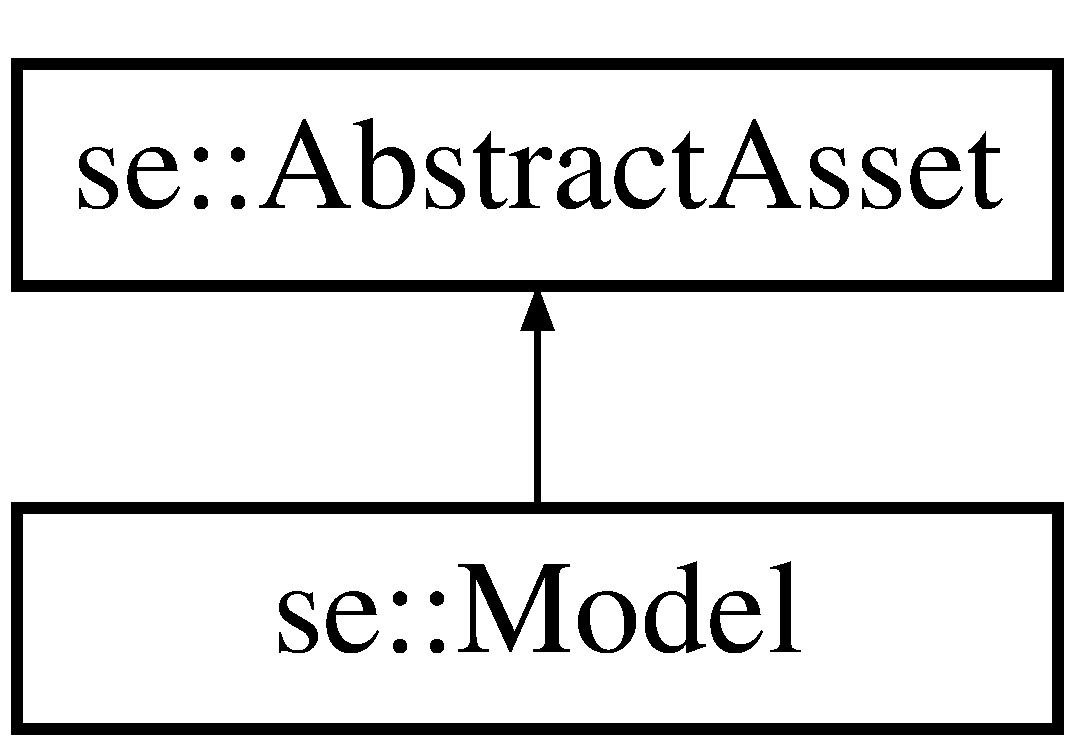
\includegraphics[height=2.000000cm]{classse_1_1_model}
\end{center}
\end{figure}
\subsection*{Public Member Functions}
\begin{DoxyCompactItemize}
\item 
\mbox{\hyperlink{classse_1_1_model_ad3008603c6880370d89d1e0eee7243df}{Model}} (\mbox{\hyperlink{classse_1_1_abstract_renderer}{Abstract\+Renderer}} $\ast$renderer, const std\+::string \&asset\+Name, const std\+::string \&path)
\end{DoxyCompactItemize}
\subsection*{Additional Inherited Members}


\subsection{Detailed Description}
A default model asset. 

Definition at line 14 of file Model.\+h.



\subsection{Constructor \& Destructor Documentation}
\mbox{\Hypertarget{classse_1_1_model_ad3008603c6880370d89d1e0eee7243df}\label{classse_1_1_model_ad3008603c6880370d89d1e0eee7243df}} 
\index{se\+::\+Model@{se\+::\+Model}!Model@{Model}}
\index{Model@{Model}!se\+::\+Model@{se\+::\+Model}}
\subsubsection{\texorpdfstring{Model()}{Model()}}
{\footnotesize\ttfamily se\+::\+Model\+::\+Model (\begin{DoxyParamCaption}\item[{\mbox{\hyperlink{classse_1_1_abstract_renderer}{Abstract\+Renderer}} $\ast$}]{renderer,  }\item[{const std\+::string \&}]{asset\+Name,  }\item[{const std\+::string \&}]{path }\end{DoxyParamCaption})}

Create a model with a renderer and the path to the model you want to load. 

Definition at line 5 of file Model.\+cpp.



The documentation for this class was generated from the following files\+:\begin{DoxyCompactItemize}
\item 
D\+:/\+Projects/\+Game\+Engine3\+D/\+Include/\mbox{\hyperlink{_model_8h}{Model.\+h}}\item 
D\+:/\+Projects/\+Game\+Engine3\+D/\+Source/\mbox{\hyperlink{_model_8cpp}{Model.\+cpp}}\end{DoxyCompactItemize}

\hypertarget{classse_1_1_scene}{}\section{se\+:\+:Scene Class Reference}
\label{classse_1_1_scene}\index{se\+::\+Scene@{se\+::\+Scene}}


{\ttfamily \#include $<$Scene.\+h$>$}

\subsection*{Public Member Functions}
\begin{DoxyCompactItemize}
\item 
void \mbox{\hyperlink{classse_1_1_scene_a21dde7d731d672d4c424397850864549}{Add\+Entity}} (\mbox{\hyperlink{classse_1_1_entity}{Entity}} $\ast$entity)
\item 
void \mbox{\hyperlink{classse_1_1_scene_acdc3858f5d4fd76cf9a712a02218341a}{Update}} (float delta)
\item 
void \mbox{\hyperlink{classse_1_1_scene_a4133b3e65c59229d8926dde7976ec004}{Remove}} (\mbox{\hyperlink{classse_1_1_entity}{Entity}} $\ast$entity)
\item 
void \mbox{\hyperlink{classse_1_1_scene_a73f7789f2585e65174380be509b88435}{Remove}} ()
\item 
const std\+::vector$<$ \mbox{\hyperlink{classse_1_1_entity}{Entity}} $\ast$ $>$ \& \mbox{\hyperlink{classse_1_1_scene_a1367cf1066c13c94fde1236b5dd5b208}{Get\+Entities}} () const
\end{DoxyCompactItemize}


\subsection{Detailed Description}
A scene that can have multiple entities in it. 

Definition at line 12 of file Scene.\+h.



\subsection{Member Function Documentation}
\mbox{\Hypertarget{classse_1_1_scene_a21dde7d731d672d4c424397850864549}\label{classse_1_1_scene_a21dde7d731d672d4c424397850864549}} 
\index{se\+::\+Scene@{se\+::\+Scene}!Add\+Entity@{Add\+Entity}}
\index{Add\+Entity@{Add\+Entity}!se\+::\+Scene@{se\+::\+Scene}}
\subsubsection{\texorpdfstring{Add\+Entity()}{AddEntity()}}
{\footnotesize\ttfamily void se\+::\+Scene\+::\+Add\+Entity (\begin{DoxyParamCaption}\item[{\mbox{\hyperlink{classse_1_1_entity}{Entity}} $\ast$}]{entity }\end{DoxyParamCaption})}

Add an entity to the scene. 

Definition at line 8 of file Scene.\+cpp.

\mbox{\Hypertarget{classse_1_1_scene_a1367cf1066c13c94fde1236b5dd5b208}\label{classse_1_1_scene_a1367cf1066c13c94fde1236b5dd5b208}} 
\index{se\+::\+Scene@{se\+::\+Scene}!Get\+Entities@{Get\+Entities}}
\index{Get\+Entities@{Get\+Entities}!se\+::\+Scene@{se\+::\+Scene}}
\subsubsection{\texorpdfstring{Get\+Entities()}{GetEntities()}}
{\footnotesize\ttfamily const std\+::vector$<$ \mbox{\hyperlink{classse_1_1_entity}{Entity}} $\ast$ $>$ \& se\+::\+Scene\+::\+Get\+Entities (\begin{DoxyParamCaption}{ }\end{DoxyParamCaption}) const}

Get all entities in the scene 

Definition at line 41 of file Scene.\+cpp.

\mbox{\Hypertarget{classse_1_1_scene_a4133b3e65c59229d8926dde7976ec004}\label{classse_1_1_scene_a4133b3e65c59229d8926dde7976ec004}} 
\index{se\+::\+Scene@{se\+::\+Scene}!Remove@{Remove}}
\index{Remove@{Remove}!se\+::\+Scene@{se\+::\+Scene}}
\subsubsection{\texorpdfstring{Remove()}{Remove()}\hspace{0.1cm}{\footnotesize\ttfamily [1/2]}}
{\footnotesize\ttfamily void se\+::\+Scene\+::\+Remove (\begin{DoxyParamCaption}\item[{\mbox{\hyperlink{classse_1_1_entity}{Entity}} $\ast$}]{entity }\end{DoxyParamCaption})}

Remove an entity from the scene. 

Definition at line 29 of file Scene.\+cpp.

\mbox{\Hypertarget{classse_1_1_scene_a73f7789f2585e65174380be509b88435}\label{classse_1_1_scene_a73f7789f2585e65174380be509b88435}} 
\index{se\+::\+Scene@{se\+::\+Scene}!Remove@{Remove}}
\index{Remove@{Remove}!se\+::\+Scene@{se\+::\+Scene}}
\subsubsection{\texorpdfstring{Remove()}{Remove()}\hspace{0.1cm}{\footnotesize\ttfamily [2/2]}}
{\footnotesize\ttfamily void se\+::\+Scene\+::\+Remove (\begin{DoxyParamCaption}{ }\end{DoxyParamCaption})}

Remove everything from the scene 

Definition at line 34 of file Scene.\+cpp.

\mbox{\Hypertarget{classse_1_1_scene_acdc3858f5d4fd76cf9a712a02218341a}\label{classse_1_1_scene_acdc3858f5d4fd76cf9a712a02218341a}} 
\index{se\+::\+Scene@{se\+::\+Scene}!Update@{Update}}
\index{Update@{Update}!se\+::\+Scene@{se\+::\+Scene}}
\subsubsection{\texorpdfstring{Update()}{Update()}}
{\footnotesize\ttfamily void se\+::\+Scene\+::\+Update (\begin{DoxyParamCaption}\item[{float}]{delta }\end{DoxyParamCaption})}

Update all entities 

Definition at line 12 of file Scene.\+cpp.



The documentation for this class was generated from the following files\+:\begin{DoxyCompactItemize}
\item 
D\+:/\+Projects/\+Game\+Engine3\+D/\+Include/\mbox{\hyperlink{_scene_8h}{Scene.\+h}}\item 
D\+:/\+Projects/\+Game\+Engine3\+D/\+Source/\mbox{\hyperlink{_scene_8cpp}{Scene.\+cpp}}\end{DoxyCompactItemize}

\hypertarget{classse_1_1_scene_loader}{}\section{se\+:\+:Scene\+Loader Class Reference}
\label{classse_1_1_scene_loader}\index{se\+::\+Scene\+Loader@{se\+::\+Scene\+Loader}}


{\ttfamily \#include $<$Scene\+Loader.\+h$>$}

\subsection*{Public Member Functions}
\begin{DoxyCompactItemize}
\item 
\mbox{\hyperlink{classse_1_1_scene_loader_a330e5c0d025a64e8386ad9d994f2dbad}{Scene\+Loader}} (\mbox{\hyperlink{classse_1_1_abstract_renderer}{Abstract\+Renderer}} $\ast$renderer, const std\+::string \&path, \mbox{\hyperlink{classse_1_1_abstract_input}{Abstract\+Input}} $\ast$input)
\end{DoxyCompactItemize}


\subsection{Detailed Description}
Load assets, scenes from an X\+ML file with this loader. 

Definition at line 16 of file Scene\+Loader.\+h.



\subsection{Constructor \& Destructor Documentation}
\mbox{\Hypertarget{classse_1_1_scene_loader_a330e5c0d025a64e8386ad9d994f2dbad}\label{classse_1_1_scene_loader_a330e5c0d025a64e8386ad9d994f2dbad}} 
\index{se\+::\+Scene\+Loader@{se\+::\+Scene\+Loader}!Scene\+Loader@{Scene\+Loader}}
\index{Scene\+Loader@{Scene\+Loader}!se\+::\+Scene\+Loader@{se\+::\+Scene\+Loader}}
\subsubsection{\texorpdfstring{Scene\+Loader()}{SceneLoader()}}
{\footnotesize\ttfamily se\+::\+Scene\+Loader\+::\+Scene\+Loader (\begin{DoxyParamCaption}\item[{\mbox{\hyperlink{classse_1_1_abstract_renderer}{Abstract\+Renderer}} $\ast$}]{renderer,  }\item[{const std\+::string \&}]{path,  }\item[{\mbox{\hyperlink{classse_1_1_abstract_input}{Abstract\+Input}} $\ast$}]{input }\end{DoxyParamCaption})}

Load the assets, scenes and entities within the scenes with the given path to the X\+ML file that contains the data to load. 

The documentation for this class was generated from the following file\+:\begin{DoxyCompactItemize}
\item 
D\+:/\+Projects/\+Game\+Engine3\+D/\+Include/\mbox{\hyperlink{_scene_loader_8h}{Scene\+Loader.\+h}}\end{DoxyCompactItemize}

\hypertarget{classse_1_1_scene_manager}{}\section{se\+:\+:Scene\+Manager Class Reference}
\label{classse_1_1_scene_manager}\index{se\+::\+Scene\+Manager@{se\+::\+Scene\+Manager}}


{\ttfamily \#include $<$Scene\+Manager.\+h$>$}

\subsection*{Public Member Functions}
\begin{DoxyCompactItemize}
\item 
\mbox{\hyperlink{classse_1_1_scene}{Scene}} $\ast$ \mbox{\hyperlink{classse_1_1_scene_manager_a07360d102e47455f497c844d7ad36ecb}{Get\+Scene}} (const std\+::string \&name)
\item 
void \mbox{\hyperlink{classse_1_1_scene_manager_a9ad26f193f547285f4eae5c440f24a10}{Add\+Scene}} (const std\+::string \&name)
\item 
void \mbox{\hyperlink{classse_1_1_scene_manager_a8eff0a05036942247f81fe4915ffce50}{Set\+Current\+Scene}} (const std\+::string \&name)
\item 
int \mbox{\hyperlink{classse_1_1_scene_manager_aac6929d7dfd933c4d40fbf66b3740321}{Get\+Scene\+Count}} ()
\end{DoxyCompactItemize}
\subsection*{Static Public Member Functions}
\begin{DoxyCompactItemize}
\item 
static \mbox{\hyperlink{classse_1_1_scene_manager}{Scene\+Manager}} $\ast$ \mbox{\hyperlink{classse_1_1_scene_manager_a670006ca4d20028e0778074e94fa0640}{Get\+Instance}} ()
\item 
static \mbox{\hyperlink{classse_1_1_scene}{Scene}} $\ast$ \mbox{\hyperlink{classse_1_1_scene_manager_a79b72ff927600fa9ef24f1dae177b566}{Get\+Current\+Scene}} ()
\end{DoxyCompactItemize}


\subsection{Detailed Description}


Definition at line 10 of file Scene\+Manager.\+h.



\subsection{Member Function Documentation}
\mbox{\Hypertarget{classse_1_1_scene_manager_a9ad26f193f547285f4eae5c440f24a10}\label{classse_1_1_scene_manager_a9ad26f193f547285f4eae5c440f24a10}} 
\index{se\+::\+Scene\+Manager@{se\+::\+Scene\+Manager}!Add\+Scene@{Add\+Scene}}
\index{Add\+Scene@{Add\+Scene}!se\+::\+Scene\+Manager@{se\+::\+Scene\+Manager}}
\subsubsection{\texorpdfstring{Add\+Scene()}{AddScene()}}
{\footnotesize\ttfamily void se\+::\+Scene\+Manager\+::\+Add\+Scene (\begin{DoxyParamCaption}\item[{const std\+::string \&}]{name }\end{DoxyParamCaption})}

\mbox{\Hypertarget{classse_1_1_scene_manager_a79b72ff927600fa9ef24f1dae177b566}\label{classse_1_1_scene_manager_a79b72ff927600fa9ef24f1dae177b566}} 
\index{se\+::\+Scene\+Manager@{se\+::\+Scene\+Manager}!Get\+Current\+Scene@{Get\+Current\+Scene}}
\index{Get\+Current\+Scene@{Get\+Current\+Scene}!se\+::\+Scene\+Manager@{se\+::\+Scene\+Manager}}
\subsubsection{\texorpdfstring{Get\+Current\+Scene()}{GetCurrentScene()}}
{\footnotesize\ttfamily static \mbox{\hyperlink{classse_1_1_scene}{Scene}}$\ast$ se\+::\+Scene\+Manager\+::\+Get\+Current\+Scene (\begin{DoxyParamCaption}{ }\end{DoxyParamCaption})\hspace{0.3cm}{\ttfamily [static]}}

\mbox{\Hypertarget{classse_1_1_scene_manager_a670006ca4d20028e0778074e94fa0640}\label{classse_1_1_scene_manager_a670006ca4d20028e0778074e94fa0640}} 
\index{se\+::\+Scene\+Manager@{se\+::\+Scene\+Manager}!Get\+Instance@{Get\+Instance}}
\index{Get\+Instance@{Get\+Instance}!se\+::\+Scene\+Manager@{se\+::\+Scene\+Manager}}
\subsubsection{\texorpdfstring{Get\+Instance()}{GetInstance()}}
{\footnotesize\ttfamily static \mbox{\hyperlink{classse_1_1_scene_manager}{Scene\+Manager}}$\ast$ se\+::\+Scene\+Manager\+::\+Get\+Instance (\begin{DoxyParamCaption}{ }\end{DoxyParamCaption})\hspace{0.3cm}{\ttfamily [static]}}

\mbox{\Hypertarget{classse_1_1_scene_manager_a07360d102e47455f497c844d7ad36ecb}\label{classse_1_1_scene_manager_a07360d102e47455f497c844d7ad36ecb}} 
\index{se\+::\+Scene\+Manager@{se\+::\+Scene\+Manager}!Get\+Scene@{Get\+Scene}}
\index{Get\+Scene@{Get\+Scene}!se\+::\+Scene\+Manager@{se\+::\+Scene\+Manager}}
\subsubsection{\texorpdfstring{Get\+Scene()}{GetScene()}}
{\footnotesize\ttfamily \mbox{\hyperlink{classse_1_1_scene}{Scene}}$\ast$ se\+::\+Scene\+Manager\+::\+Get\+Scene (\begin{DoxyParamCaption}\item[{const std\+::string \&}]{name }\end{DoxyParamCaption})}

\mbox{\Hypertarget{classse_1_1_scene_manager_aac6929d7dfd933c4d40fbf66b3740321}\label{classse_1_1_scene_manager_aac6929d7dfd933c4d40fbf66b3740321}} 
\index{se\+::\+Scene\+Manager@{se\+::\+Scene\+Manager}!Get\+Scene\+Count@{Get\+Scene\+Count}}
\index{Get\+Scene\+Count@{Get\+Scene\+Count}!se\+::\+Scene\+Manager@{se\+::\+Scene\+Manager}}
\subsubsection{\texorpdfstring{Get\+Scene\+Count()}{GetSceneCount()}}
{\footnotesize\ttfamily int se\+::\+Scene\+Manager\+::\+Get\+Scene\+Count (\begin{DoxyParamCaption}{ }\end{DoxyParamCaption})}

\mbox{\Hypertarget{classse_1_1_scene_manager_a8eff0a05036942247f81fe4915ffce50}\label{classse_1_1_scene_manager_a8eff0a05036942247f81fe4915ffce50}} 
\index{se\+::\+Scene\+Manager@{se\+::\+Scene\+Manager}!Set\+Current\+Scene@{Set\+Current\+Scene}}
\index{Set\+Current\+Scene@{Set\+Current\+Scene}!se\+::\+Scene\+Manager@{se\+::\+Scene\+Manager}}
\subsubsection{\texorpdfstring{Set\+Current\+Scene()}{SetCurrentScene()}}
{\footnotesize\ttfamily void se\+::\+Scene\+Manager\+::\+Set\+Current\+Scene (\begin{DoxyParamCaption}\item[{const std\+::string \&}]{name }\end{DoxyParamCaption})}



The documentation for this class was generated from the following file\+:\begin{DoxyCompactItemize}
\item 
Include/\mbox{\hyperlink{_scene_manager_8h}{Scene\+Manager.\+h}}\end{DoxyCompactItemize}

\hypertarget{classse_1_1_skybox}{}\section{se\+:\+:Skybox Class Reference}
\label{classse_1_1_skybox}\index{se\+::\+Skybox@{se\+::\+Skybox}}


{\ttfamily \#include $<$Skybox.\+h$>$}

Inheritance diagram for se\+:\+:Skybox\+:\begin{figure}[H]
\begin{center}
\leavevmode
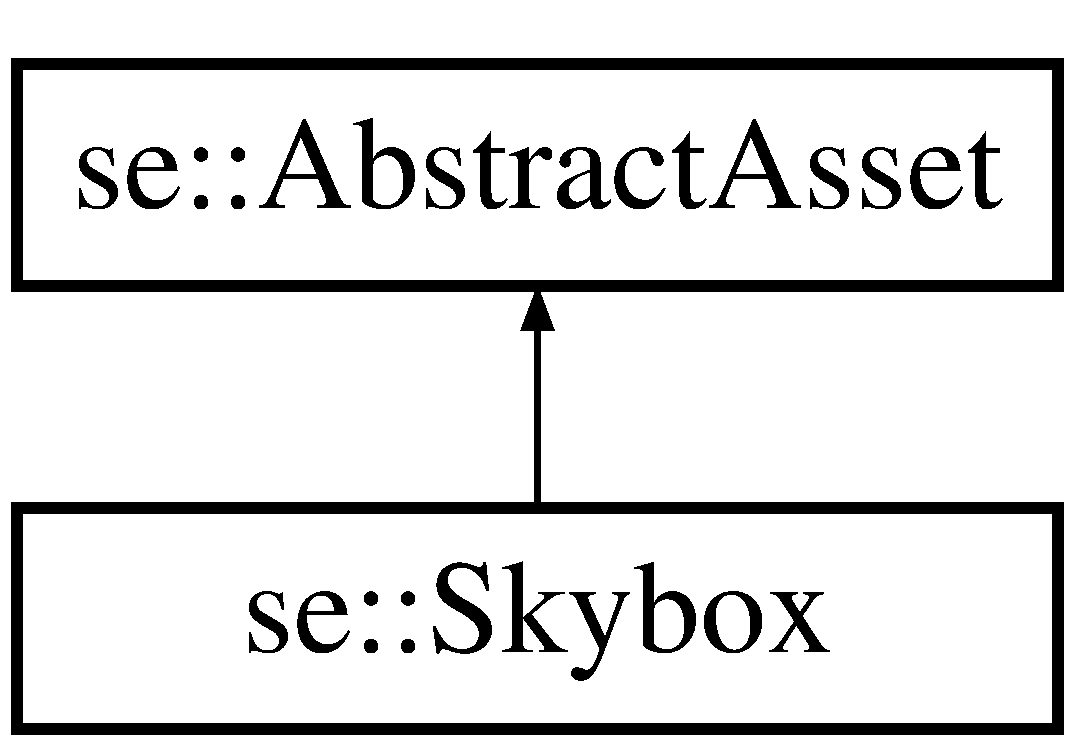
\includegraphics[height=2.000000cm]{classse_1_1_skybox}
\end{center}
\end{figure}
\subsection*{Public Member Functions}
\begin{DoxyCompactItemize}
\item 
\mbox{\hyperlink{classse_1_1_skybox_adf8ae4ca19649dd144eeefca2c78b6df}{Skybox}} (\mbox{\hyperlink{classse_1_1_abstract_renderer}{Abstract\+Renderer}} $\ast$renderer, const std\+::string \&asset\+Name, const std\+::string \&src)
\end{DoxyCompactItemize}
\subsection*{Additional Inherited Members}


\subsection{Detailed Description}
A default skybox asset. 

Definition at line 14 of file Skybox.\+h.



\subsection{Constructor \& Destructor Documentation}
\mbox{\Hypertarget{classse_1_1_skybox_adf8ae4ca19649dd144eeefca2c78b6df}\label{classse_1_1_skybox_adf8ae4ca19649dd144eeefca2c78b6df}} 
\index{se\+::\+Skybox@{se\+::\+Skybox}!Skybox@{Skybox}}
\index{Skybox@{Skybox}!se\+::\+Skybox@{se\+::\+Skybox}}
\subsubsection{\texorpdfstring{Skybox()}{Skybox()}}
{\footnotesize\ttfamily se\+::\+Skybox\+::\+Skybox (\begin{DoxyParamCaption}\item[{\mbox{\hyperlink{classse_1_1_abstract_renderer}{Abstract\+Renderer}} $\ast$}]{renderer,  }\item[{const std\+::string \&}]{asset\+Name,  }\item[{const std\+::string \&}]{src }\end{DoxyParamCaption})}

Create a skybox with a renderer and a cubemap. 

Definition at line 5 of file Skybox.\+cpp.



The documentation for this class was generated from the following files\+:\begin{DoxyCompactItemize}
\item 
D\+:/\+Projects/\+Game\+Engine3\+D/\+Include/\mbox{\hyperlink{_skybox_8h}{Skybox.\+h}}\item 
D\+:/\+Projects/\+Game\+Engine3\+D/\+Source/\mbox{\hyperlink{_skybox_8cpp}{Skybox.\+cpp}}\end{DoxyCompactItemize}

\hypertarget{classse_1_1_terrain}{}\section{se\+:\+:Terrain Class Reference}
\label{classse_1_1_terrain}\index{se\+::\+Terrain@{se\+::\+Terrain}}


{\ttfamily \#include $<$Terrain.\+h$>$}

Inheritance diagram for se\+:\+:Terrain\+:\begin{figure}[H]
\begin{center}
\leavevmode
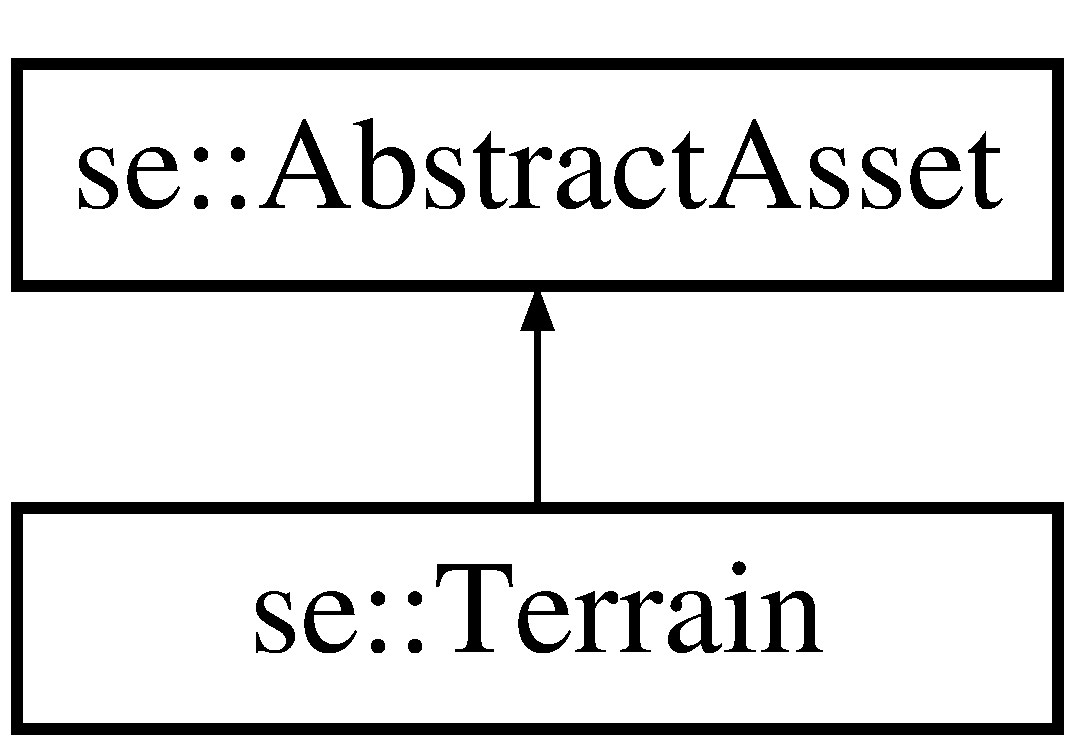
\includegraphics[height=2.000000cm]{classse_1_1_terrain}
\end{center}
\end{figure}
\subsection*{Public Member Functions}
\begin{DoxyCompactItemize}
\item 
\mbox{\hyperlink{classse_1_1_terrain_a0e20b4b0333c3d92bfe143bf3cc17b2a}{Terrain}} (\mbox{\hyperlink{classse_1_1_abstract_renderer}{Abstract\+Renderer}} $\ast$renderer, const std\+::string \&asset\+Name, const std\+::string \&height\+Map, const std\+::string \&texture)
\item 
void \mbox{\hyperlink{classse_1_1_terrain_a0fcef77b6b1d8e32ce49a396d4d733e2}{Render}} ()
\item 
void \mbox{\hyperlink{classse_1_1_terrain_aab4ebd41c3ae26b258928d8f2454ed88}{Release}} ()
\end{DoxyCompactItemize}
\subsection*{Additional Inherited Members}


\subsection{Detailed Description}
A default terrain asset. 

Definition at line 16 of file Terrain.\+h.



\subsection{Constructor \& Destructor Documentation}
\mbox{\Hypertarget{classse_1_1_terrain_a0e20b4b0333c3d92bfe143bf3cc17b2a}\label{classse_1_1_terrain_a0e20b4b0333c3d92bfe143bf3cc17b2a}} 
\index{se\+::\+Terrain@{se\+::\+Terrain}!Terrain@{Terrain}}
\index{Terrain@{Terrain}!se\+::\+Terrain@{se\+::\+Terrain}}
\subsubsection{\texorpdfstring{Terrain()}{Terrain()}}
{\footnotesize\ttfamily se\+::\+Terrain\+::\+Terrain (\begin{DoxyParamCaption}\item[{\mbox{\hyperlink{classse_1_1_abstract_renderer}{Abstract\+Renderer}} $\ast$}]{renderer,  }\item[{const std\+::string \&}]{asset\+Name,  }\item[{const std\+::string \&}]{height\+Map,  }\item[{const std\+::string \&}]{texture }\end{DoxyParamCaption})}

Create a terrain with a renderer, heightmap for the heights and texture to put on the terrain. 

\subsection{Member Function Documentation}
\mbox{\Hypertarget{classse_1_1_terrain_aab4ebd41c3ae26b258928d8f2454ed88}\label{classse_1_1_terrain_aab4ebd41c3ae26b258928d8f2454ed88}} 
\index{se\+::\+Terrain@{se\+::\+Terrain}!Release@{Release}}
\index{Release@{Release}!se\+::\+Terrain@{se\+::\+Terrain}}
\subsubsection{\texorpdfstring{Release()}{Release()}}
{\footnotesize\ttfamily void se\+::\+Terrain\+::\+Release (\begin{DoxyParamCaption}{ }\end{DoxyParamCaption})\hspace{0.3cm}{\ttfamily [virtual]}}

Release the terrain asset. 

Implements \mbox{\hyperlink{classse_1_1_abstract_asset_aea97e36f647efdb07a801b6fc468388d}{se\+::\+Abstract\+Asset}}.

\mbox{\Hypertarget{classse_1_1_terrain_a0fcef77b6b1d8e32ce49a396d4d733e2}\label{classse_1_1_terrain_a0fcef77b6b1d8e32ce49a396d4d733e2}} 
\index{se\+::\+Terrain@{se\+::\+Terrain}!Render@{Render}}
\index{Render@{Render}!se\+::\+Terrain@{se\+::\+Terrain}}
\subsubsection{\texorpdfstring{Render()}{Render()}}
{\footnotesize\ttfamily void se\+::\+Terrain\+::\+Render (\begin{DoxyParamCaption}{ }\end{DoxyParamCaption})\hspace{0.3cm}{\ttfamily [virtual]}}

Render the terrain asset. 

Implements \mbox{\hyperlink{classse_1_1_abstract_asset_a2addad2ca18a3ffbcbe1e80afa0ad56c}{se\+::\+Abstract\+Asset}}.



The documentation for this class was generated from the following file\+:\begin{DoxyCompactItemize}
\item 
D\+:/\+Projects/\+Game\+Engine3\+D/\+Include/\mbox{\hyperlink{_terrain_8h}{Terrain.\+h}}\end{DoxyCompactItemize}

\hypertarget{classse_1_1_timer}{}\section{se\+:\+:Timer Class Reference}
\label{classse_1_1_timer}\index{se\+::\+Timer@{se\+::\+Timer}}


{\ttfamily \#include $<$Timer.\+h$>$}

\subsection*{Public Member Functions}
\begin{DoxyCompactItemize}
\item 
\mbox{\hyperlink{classse_1_1_timer_a0f3bf62bd9419c252910191f13669dd7}{Timer}} ()
\item 
void \mbox{\hyperlink{classse_1_1_timer_a0294f5629a28a1e169a8d1b5ab179273}{Start}} ()
\item 
void \mbox{\hyperlink{classse_1_1_timer_abde91d5d6e7fe0601c0c9607193707d8}{Pause}} ()
\item 
void \mbox{\hyperlink{classse_1_1_timer_a432406f463e02336c1033d65ae1d746e}{Resume}} ()
\item 
void \mbox{\hyperlink{classse_1_1_timer_aed6b34f75ec989731c80fefe962493f3}{Stop}} ()
\item 
long long \mbox{\hyperlink{classse_1_1_timer_a7fdf38aafc8be894fc25764ff8cabb36}{Microseconds}} ()
\item 
long long \mbox{\hyperlink{classse_1_1_timer_a9c3fe064b6637f2804c370da786a38d8}{Milliseconds}} ()
\item 
long long \mbox{\hyperlink{classse_1_1_timer_a258761c48271338588503d8170532bde}{Seconds}} ()
\end{DoxyCompactItemize}


\subsection{Detailed Description}
You can use this class to get the time elapsed from the specified start. 

Definition at line 9 of file Timer.\+h.



\subsection{Constructor \& Destructor Documentation}
\mbox{\Hypertarget{classse_1_1_timer_a0f3bf62bd9419c252910191f13669dd7}\label{classse_1_1_timer_a0f3bf62bd9419c252910191f13669dd7}} 
\index{se\+::\+Timer@{se\+::\+Timer}!Timer@{Timer}}
\index{Timer@{Timer}!se\+::\+Timer@{se\+::\+Timer}}
\subsubsection{\texorpdfstring{Timer()}{Timer()}}
{\footnotesize\ttfamily se\+::\+Timer\+::\+Timer (\begin{DoxyParamCaption}{ }\end{DoxyParamCaption})}



Definition at line 6 of file Timer.\+cpp.



\subsection{Member Function Documentation}
\mbox{\Hypertarget{classse_1_1_timer_a7fdf38aafc8be894fc25764ff8cabb36}\label{classse_1_1_timer_a7fdf38aafc8be894fc25764ff8cabb36}} 
\index{se\+::\+Timer@{se\+::\+Timer}!Microseconds@{Microseconds}}
\index{Microseconds@{Microseconds}!se\+::\+Timer@{se\+::\+Timer}}
\subsubsection{\texorpdfstring{Microseconds()}{Microseconds()}}
{\footnotesize\ttfamily long long se\+::\+Timer\+::\+Microseconds (\begin{DoxyParamCaption}{ }\end{DoxyParamCaption})}

Get the microseconds passed. 

Definition at line 46 of file Timer.\+cpp.

\mbox{\Hypertarget{classse_1_1_timer_a9c3fe064b6637f2804c370da786a38d8}\label{classse_1_1_timer_a9c3fe064b6637f2804c370da786a38d8}} 
\index{se\+::\+Timer@{se\+::\+Timer}!Milliseconds@{Milliseconds}}
\index{Milliseconds@{Milliseconds}!se\+::\+Timer@{se\+::\+Timer}}
\subsubsection{\texorpdfstring{Milliseconds()}{Milliseconds()}}
{\footnotesize\ttfamily long long se\+::\+Timer\+::\+Milliseconds (\begin{DoxyParamCaption}{ }\end{DoxyParamCaption})}

Get the milliseconds passed. 

Definition at line 57 of file Timer.\+cpp.

\mbox{\Hypertarget{classse_1_1_timer_abde91d5d6e7fe0601c0c9607193707d8}\label{classse_1_1_timer_abde91d5d6e7fe0601c0c9607193707d8}} 
\index{se\+::\+Timer@{se\+::\+Timer}!Pause@{Pause}}
\index{Pause@{Pause}!se\+::\+Timer@{se\+::\+Timer}}
\subsubsection{\texorpdfstring{Pause()}{Pause()}}
{\footnotesize\ttfamily void se\+::\+Timer\+::\+Pause (\begin{DoxyParamCaption}{ }\end{DoxyParamCaption})}

Pause the timer. 

Definition at line 32 of file Timer.\+cpp.

\mbox{\Hypertarget{classse_1_1_timer_a432406f463e02336c1033d65ae1d746e}\label{classse_1_1_timer_a432406f463e02336c1033d65ae1d746e}} 
\index{se\+::\+Timer@{se\+::\+Timer}!Resume@{Resume}}
\index{Resume@{Resume}!se\+::\+Timer@{se\+::\+Timer}}
\subsubsection{\texorpdfstring{Resume()}{Resume()}}
{\footnotesize\ttfamily void se\+::\+Timer\+::\+Resume (\begin{DoxyParamCaption}{ }\end{DoxyParamCaption})}

Resume the timer. 

Definition at line 41 of file Timer.\+cpp.

\mbox{\Hypertarget{classse_1_1_timer_a258761c48271338588503d8170532bde}\label{classse_1_1_timer_a258761c48271338588503d8170532bde}} 
\index{se\+::\+Timer@{se\+::\+Timer}!Seconds@{Seconds}}
\index{Seconds@{Seconds}!se\+::\+Timer@{se\+::\+Timer}}
\subsubsection{\texorpdfstring{Seconds()}{Seconds()}}
{\footnotesize\ttfamily long long se\+::\+Timer\+::\+Seconds (\begin{DoxyParamCaption}{ }\end{DoxyParamCaption})}

Get the seconds passed. 

Definition at line 61 of file Timer.\+cpp.

\mbox{\Hypertarget{classse_1_1_timer_a0294f5629a28a1e169a8d1b5ab179273}\label{classse_1_1_timer_a0294f5629a28a1e169a8d1b5ab179273}} 
\index{se\+::\+Timer@{se\+::\+Timer}!Start@{Start}}
\index{Start@{Start}!se\+::\+Timer@{se\+::\+Timer}}
\subsubsection{\texorpdfstring{Start()}{Start()}}
{\footnotesize\ttfamily void se\+::\+Timer\+::\+Start (\begin{DoxyParamCaption}{ }\end{DoxyParamCaption})}

Start the timer. 

Definition at line 14 of file Timer.\+cpp.

\mbox{\Hypertarget{classse_1_1_timer_aed6b34f75ec989731c80fefe962493f3}\label{classse_1_1_timer_aed6b34f75ec989731c80fefe962493f3}} 
\index{se\+::\+Timer@{se\+::\+Timer}!Stop@{Stop}}
\index{Stop@{Stop}!se\+::\+Timer@{se\+::\+Timer}}
\subsubsection{\texorpdfstring{Stop()}{Stop()}}
{\footnotesize\ttfamily void se\+::\+Timer\+::\+Stop (\begin{DoxyParamCaption}{ }\end{DoxyParamCaption})}

Stop the timer. 

Definition at line 22 of file Timer.\+cpp.



The documentation for this class was generated from the following files\+:\begin{DoxyCompactItemize}
\item 
D\+:/\+Projects/\+Game\+Engine3\+D/\+Include/\mbox{\hyperlink{_timer_8h}{Timer.\+h}}\item 
D\+:/\+Projects/\+Game\+Engine3\+D/\+Source/\mbox{\hyperlink{_timer_8cpp}{Timer.\+cpp}}\end{DoxyCompactItemize}

\hypertarget{classse_1_1_vector3}{}\section{se\+:\+:Vector3$<$ T $>$ Class Template Reference}
\label{classse_1_1_vector3}\index{se\+::\+Vector3$<$ T $>$@{se\+::\+Vector3$<$ T $>$}}


{\ttfamily \#include $<$Vector3.\+h$>$}

\subsection*{Public Member Functions}
\begin{DoxyCompactItemize}
\item 
\mbox{\hyperlink{classse_1_1_vector3_a9287277a349e2e99447b3eafe69bff5a}{Vector3}} ()
\item 
\mbox{\hyperlink{classse_1_1_vector3_a6d5f0d6aded9d084a39013c928515724}{Vector3}} (T \mbox{\hyperlink{classse_1_1_vector3_a1dd0e9af86e73921dd391b00dbfd8526}{x}}, T \mbox{\hyperlink{classse_1_1_vector3_a32fd129ef6071a9316612fa223e2ca1b}{y}}, T \mbox{\hyperlink{classse_1_1_vector3_ac38fc2b30fc8426e66746a6220b21a03}{z}})
\item 
void \mbox{\hyperlink{classse_1_1_vector3_a413a3535ea9c8a76ef2f4d8c782684b8}{Set}} (T \mbox{\hyperlink{classse_1_1_vector3_a1dd0e9af86e73921dd391b00dbfd8526}{x}}, T \mbox{\hyperlink{classse_1_1_vector3_a32fd129ef6071a9316612fa223e2ca1b}{y}}, T \mbox{\hyperlink{classse_1_1_vector3_ac38fc2b30fc8426e66746a6220b21a03}{z}})
\end{DoxyCompactItemize}
\subsection*{Public Attributes}
\begin{DoxyCompactItemize}
\item 
T \mbox{\hyperlink{classse_1_1_vector3_a1dd0e9af86e73921dd391b00dbfd8526}{x}}
\item 
T \mbox{\hyperlink{classse_1_1_vector3_a32fd129ef6071a9316612fa223e2ca1b}{y}}
\item 
T \mbox{\hyperlink{classse_1_1_vector3_ac38fc2b30fc8426e66746a6220b21a03}{z}}
\end{DoxyCompactItemize}


\subsection{Detailed Description}
\subsubsection*{template$<$class T$>$\newline
class se\+::\+Vector3$<$ T $>$}

For all your transformation needs. 

Definition at line 10 of file Vector3.\+h.



\subsection{Constructor \& Destructor Documentation}
\mbox{\Hypertarget{classse_1_1_vector3_a9287277a349e2e99447b3eafe69bff5a}\label{classse_1_1_vector3_a9287277a349e2e99447b3eafe69bff5a}} 
\index{se\+::\+Vector3@{se\+::\+Vector3}!Vector3@{Vector3}}
\index{Vector3@{Vector3}!se\+::\+Vector3@{se\+::\+Vector3}}
\subsubsection{\texorpdfstring{Vector3()}{Vector3()}\hspace{0.1cm}{\footnotesize\ttfamily [1/2]}}
{\footnotesize\ttfamily template$<$class T$>$ \\
\mbox{\hyperlink{classse_1_1_vector3}{se\+::\+Vector3}}$<$ T $>$\+::\mbox{\hyperlink{classse_1_1_vector3}{Vector3}} (\begin{DoxyParamCaption}{ }\end{DoxyParamCaption})\hspace{0.3cm}{\ttfamily [inline]}}



Definition at line 14 of file Vector3.\+h.

\mbox{\Hypertarget{classse_1_1_vector3_a6d5f0d6aded9d084a39013c928515724}\label{classse_1_1_vector3_a6d5f0d6aded9d084a39013c928515724}} 
\index{se\+::\+Vector3@{se\+::\+Vector3}!Vector3@{Vector3}}
\index{Vector3@{Vector3}!se\+::\+Vector3@{se\+::\+Vector3}}
\subsubsection{\texorpdfstring{Vector3()}{Vector3()}\hspace{0.1cm}{\footnotesize\ttfamily [2/2]}}
{\footnotesize\ttfamily template$<$class T$>$ \\
\mbox{\hyperlink{classse_1_1_vector3}{se\+::\+Vector3}}$<$ T $>$\+::\mbox{\hyperlink{classse_1_1_vector3}{Vector3}} (\begin{DoxyParamCaption}\item[{T}]{x,  }\item[{T}]{y,  }\item[{T}]{z }\end{DoxyParamCaption})\hspace{0.3cm}{\ttfamily [inline]}}



Definition at line 20 of file Vector3.\+h.



\subsection{Member Function Documentation}
\mbox{\Hypertarget{classse_1_1_vector3_a413a3535ea9c8a76ef2f4d8c782684b8}\label{classse_1_1_vector3_a413a3535ea9c8a76ef2f4d8c782684b8}} 
\index{se\+::\+Vector3@{se\+::\+Vector3}!Set@{Set}}
\index{Set@{Set}!se\+::\+Vector3@{se\+::\+Vector3}}
\subsubsection{\texorpdfstring{Set()}{Set()}}
{\footnotesize\ttfamily template$<$class T$>$ \\
void \mbox{\hyperlink{classse_1_1_vector3}{se\+::\+Vector3}}$<$ T $>$\+::Set (\begin{DoxyParamCaption}\item[{T}]{x,  }\item[{T}]{y,  }\item[{T}]{z }\end{DoxyParamCaption})\hspace{0.3cm}{\ttfamily [inline]}}



Definition at line 26 of file Vector3.\+h.



\subsection{Member Data Documentation}
\mbox{\Hypertarget{classse_1_1_vector3_a1dd0e9af86e73921dd391b00dbfd8526}\label{classse_1_1_vector3_a1dd0e9af86e73921dd391b00dbfd8526}} 
\index{se\+::\+Vector3@{se\+::\+Vector3}!x@{x}}
\index{x@{x}!se\+::\+Vector3@{se\+::\+Vector3}}
\subsubsection{\texorpdfstring{x}{x}}
{\footnotesize\ttfamily template$<$class T$>$ \\
T \mbox{\hyperlink{classse_1_1_vector3}{se\+::\+Vector3}}$<$ T $>$\+::x}



Definition at line 12 of file Vector3.\+h.

\mbox{\Hypertarget{classse_1_1_vector3_a32fd129ef6071a9316612fa223e2ca1b}\label{classse_1_1_vector3_a32fd129ef6071a9316612fa223e2ca1b}} 
\index{se\+::\+Vector3@{se\+::\+Vector3}!y@{y}}
\index{y@{y}!se\+::\+Vector3@{se\+::\+Vector3}}
\subsubsection{\texorpdfstring{y}{y}}
{\footnotesize\ttfamily template$<$class T$>$ \\
T \mbox{\hyperlink{classse_1_1_vector3}{se\+::\+Vector3}}$<$ T $>$\+::y}



Definition at line 12 of file Vector3.\+h.

\mbox{\Hypertarget{classse_1_1_vector3_ac38fc2b30fc8426e66746a6220b21a03}\label{classse_1_1_vector3_ac38fc2b30fc8426e66746a6220b21a03}} 
\index{se\+::\+Vector3@{se\+::\+Vector3}!z@{z}}
\index{z@{z}!se\+::\+Vector3@{se\+::\+Vector3}}
\subsubsection{\texorpdfstring{z}{z}}
{\footnotesize\ttfamily template$<$class T$>$ \\
T \mbox{\hyperlink{classse_1_1_vector3}{se\+::\+Vector3}}$<$ T $>$\+::z}



Definition at line 12 of file Vector3.\+h.



The documentation for this class was generated from the following file\+:\begin{DoxyCompactItemize}
\item 
D\+:/\+Projects/\+Game\+Engine3\+D/\+Include/\mbox{\hyperlink{_vector3_8h}{Vector3.\+h}}\end{DoxyCompactItemize}

\hypertarget{structse_1_1_vertex}{}\section{se\+:\+:Vertex Struct Reference}
\label{structse_1_1_vertex}\index{se\+::\+Vertex@{se\+::\+Vertex}}
\subsection*{Public Attributes}
\begin{DoxyCompactItemize}
\item 
float \mbox{\hyperlink{structse_1_1_vertex_a861f929c19a2002c84cc45937af25ccd}{x}}
\item 
float \mbox{\hyperlink{structse_1_1_vertex_a6e79ab7f589edb89969385db39405297}{y}}
\item 
float \mbox{\hyperlink{structse_1_1_vertex_a2a709adb9f77c1611363a550e658983b}{z}}
\item 
float \mbox{\hyperlink{structse_1_1_vertex_a8c002af2126ae5cd8dac03ec2adcb060}{tu}}
\item 
float \mbox{\hyperlink{structse_1_1_vertex_abd48156d7a9e157ca38d4c4de2101524}{tv}}
\end{DoxyCompactItemize}


\subsection{Detailed Description}


Definition at line 5 of file Direct\+X\+Skybox.\+cpp.



\subsection{Member Data Documentation}
\mbox{\Hypertarget{structse_1_1_vertex_a8c002af2126ae5cd8dac03ec2adcb060}\label{structse_1_1_vertex_a8c002af2126ae5cd8dac03ec2adcb060}} 
\index{se\+::\+Vertex@{se\+::\+Vertex}!tu@{tu}}
\index{tu@{tu}!se\+::\+Vertex@{se\+::\+Vertex}}
\subsubsection{\texorpdfstring{tu}{tu}}
{\footnotesize\ttfamily float se\+::\+Vertex\+::tu}



Definition at line 9 of file Direct\+X\+Skybox.\+cpp.

\mbox{\Hypertarget{structse_1_1_vertex_abd48156d7a9e157ca38d4c4de2101524}\label{structse_1_1_vertex_abd48156d7a9e157ca38d4c4de2101524}} 
\index{se\+::\+Vertex@{se\+::\+Vertex}!tv@{tv}}
\index{tv@{tv}!se\+::\+Vertex@{se\+::\+Vertex}}
\subsubsection{\texorpdfstring{tv}{tv}}
{\footnotesize\ttfamily float se\+::\+Vertex\+::tv}



Definition at line 10 of file Direct\+X\+Skybox.\+cpp.

\mbox{\Hypertarget{structse_1_1_vertex_a861f929c19a2002c84cc45937af25ccd}\label{structse_1_1_vertex_a861f929c19a2002c84cc45937af25ccd}} 
\index{se\+::\+Vertex@{se\+::\+Vertex}!x@{x}}
\index{x@{x}!se\+::\+Vertex@{se\+::\+Vertex}}
\subsubsection{\texorpdfstring{x}{x}}
{\footnotesize\ttfamily float se\+::\+Vertex\+::x}



Definition at line 6 of file Direct\+X\+Skybox.\+cpp.

\mbox{\Hypertarget{structse_1_1_vertex_a6e79ab7f589edb89969385db39405297}\label{structse_1_1_vertex_a6e79ab7f589edb89969385db39405297}} 
\index{se\+::\+Vertex@{se\+::\+Vertex}!y@{y}}
\index{y@{y}!se\+::\+Vertex@{se\+::\+Vertex}}
\subsubsection{\texorpdfstring{y}{y}}
{\footnotesize\ttfamily float se\+::\+Vertex\+::y}



Definition at line 7 of file Direct\+X\+Skybox.\+cpp.

\mbox{\Hypertarget{structse_1_1_vertex_a2a709adb9f77c1611363a550e658983b}\label{structse_1_1_vertex_a2a709adb9f77c1611363a550e658983b}} 
\index{se\+::\+Vertex@{se\+::\+Vertex}!z@{z}}
\index{z@{z}!se\+::\+Vertex@{se\+::\+Vertex}}
\subsubsection{\texorpdfstring{z}{z}}
{\footnotesize\ttfamily float se\+::\+Vertex\+::z}



Definition at line 8 of file Direct\+X\+Skybox.\+cpp.



The documentation for this struct was generated from the following files\+:\begin{DoxyCompactItemize}
\item 
Source/\+Direct\+X9/\mbox{\hyperlink{_direct_x_skybox_8cpp}{Direct\+X\+Skybox.\+cpp}}\item 
Source/\+Direct\+X9/\mbox{\hyperlink{_direct_x_terrain_8cpp}{Direct\+X\+Terrain.\+cpp}}\end{DoxyCompactItemize}

\hypertarget{classse_1_1_window}{}\section{se\+:\+:Window Class Reference}
\label{classse_1_1_window}\index{se\+::\+Window@{se\+::\+Window}}


{\ttfamily \#include $<$Window.\+h$>$}

\subsection*{Public Member Functions}
\begin{DoxyCompactItemize}
\item 
\mbox{\hyperlink{classse_1_1_window_a903d67c495507f0ece8d2976a33b8540}{Window}} ()
\item 
H\+W\+ND \mbox{\hyperlink{classse_1_1_window_a0bc98ce202ef1c431fe2780d53dbe7da}{Open\+Window}} (const std\+::string \&title, int width, int height)
\item 
H\+I\+N\+S\+T\+A\+N\+CE \mbox{\hyperlink{classse_1_1_window_af85337c4cc5eae56412a5bbcbf471ae6}{Get\+Instance}} ()
\item 
std\+::vector$<$ \mbox{\hyperlink{structse_1_1_window_handle}{Window\+Handle}} $>$ \mbox{\hyperlink{classse_1_1_window_a3469863d327e48f06837f772d066e1e7}{Get\+Window\+List}} () const
\item 
void \mbox{\hyperlink{classse_1_1_window_a12c371c25615c9d4744a961dab9d949c}{Set\+Position}} (int index, int x, int y)
\item 
void \mbox{\hyperlink{classse_1_1_window_ac5e7a7985934606074e9c65f83f45260}{Set\+Size}} (int index, int width, int height)
\item 
void \mbox{\hyperlink{classse_1_1_window_aab3319947ce4e9cd78f16cd9be9481e5}{Close\+Window}} (int index)
\item 
void \mbox{\hyperlink{classse_1_1_window_aa36e57777577f2b0cf355461b3b0f9a3}{Close\+All}} ()
\end{DoxyCompactItemize}


\subsection{Detailed Description}
You can use this to create a window 

Definition at line 20 of file Window.\+h.



\subsection{Constructor \& Destructor Documentation}
\mbox{\Hypertarget{classse_1_1_window_a903d67c495507f0ece8d2976a33b8540}\label{classse_1_1_window_a903d67c495507f0ece8d2976a33b8540}} 
\index{se\+::\+Window@{se\+::\+Window}!Window@{Window}}
\index{Window@{Window}!se\+::\+Window@{se\+::\+Window}}
\subsubsection{\texorpdfstring{Window()}{Window()}}
{\footnotesize\ttfamily se\+::\+Window\+::\+Window (\begin{DoxyParamCaption}{ }\end{DoxyParamCaption})}



\subsection{Member Function Documentation}
\mbox{\Hypertarget{classse_1_1_window_aa36e57777577f2b0cf355461b3b0f9a3}\label{classse_1_1_window_aa36e57777577f2b0cf355461b3b0f9a3}} 
\index{se\+::\+Window@{se\+::\+Window}!Close\+All@{Close\+All}}
\index{Close\+All@{Close\+All}!se\+::\+Window@{se\+::\+Window}}
\subsubsection{\texorpdfstring{Close\+All()}{CloseAll()}}
{\footnotesize\ttfamily void se\+::\+Window\+::\+Close\+All (\begin{DoxyParamCaption}{ }\end{DoxyParamCaption})}

Close all windows \mbox{\Hypertarget{classse_1_1_window_aab3319947ce4e9cd78f16cd9be9481e5}\label{classse_1_1_window_aab3319947ce4e9cd78f16cd9be9481e5}} 
\index{se\+::\+Window@{se\+::\+Window}!Close\+Window@{Close\+Window}}
\index{Close\+Window@{Close\+Window}!se\+::\+Window@{se\+::\+Window}}
\subsubsection{\texorpdfstring{Close\+Window()}{CloseWindow()}}
{\footnotesize\ttfamily void se\+::\+Window\+::\+Close\+Window (\begin{DoxyParamCaption}\item[{int}]{index }\end{DoxyParamCaption})}

Close a specified window \mbox{\Hypertarget{classse_1_1_window_af85337c4cc5eae56412a5bbcbf471ae6}\label{classse_1_1_window_af85337c4cc5eae56412a5bbcbf471ae6}} 
\index{se\+::\+Window@{se\+::\+Window}!Get\+Instance@{Get\+Instance}}
\index{Get\+Instance@{Get\+Instance}!se\+::\+Window@{se\+::\+Window}}
\subsubsection{\texorpdfstring{Get\+Instance()}{GetInstance()}}
{\footnotesize\ttfamily H\+I\+N\+S\+T\+A\+N\+CE se\+::\+Window\+::\+Get\+Instance (\begin{DoxyParamCaption}{ }\end{DoxyParamCaption})}

Get the instance of the window \mbox{\Hypertarget{classse_1_1_window_a3469863d327e48f06837f772d066e1e7}\label{classse_1_1_window_a3469863d327e48f06837f772d066e1e7}} 
\index{se\+::\+Window@{se\+::\+Window}!Get\+Window\+List@{Get\+Window\+List}}
\index{Get\+Window\+List@{Get\+Window\+List}!se\+::\+Window@{se\+::\+Window}}
\subsubsection{\texorpdfstring{Get\+Window\+List()}{GetWindowList()}}
{\footnotesize\ttfamily std\+::vector$<$\mbox{\hyperlink{structse_1_1_window_handle}{Window\+Handle}}$>$ se\+::\+Window\+::\+Get\+Window\+List (\begin{DoxyParamCaption}{ }\end{DoxyParamCaption}) const}

Get all windows \mbox{\Hypertarget{classse_1_1_window_a0bc98ce202ef1c431fe2780d53dbe7da}\label{classse_1_1_window_a0bc98ce202ef1c431fe2780d53dbe7da}} 
\index{se\+::\+Window@{se\+::\+Window}!Open\+Window@{Open\+Window}}
\index{Open\+Window@{Open\+Window}!se\+::\+Window@{se\+::\+Window}}
\subsubsection{\texorpdfstring{Open\+Window()}{OpenWindow()}}
{\footnotesize\ttfamily H\+W\+ND se\+::\+Window\+::\+Open\+Window (\begin{DoxyParamCaption}\item[{const std\+::string \&}]{title,  }\item[{int}]{width,  }\item[{int}]{height }\end{DoxyParamCaption})}

Create a new window \mbox{\Hypertarget{classse_1_1_window_a12c371c25615c9d4744a961dab9d949c}\label{classse_1_1_window_a12c371c25615c9d4744a961dab9d949c}} 
\index{se\+::\+Window@{se\+::\+Window}!Set\+Position@{Set\+Position}}
\index{Set\+Position@{Set\+Position}!se\+::\+Window@{se\+::\+Window}}
\subsubsection{\texorpdfstring{Set\+Position()}{SetPosition()}}
{\footnotesize\ttfamily void se\+::\+Window\+::\+Set\+Position (\begin{DoxyParamCaption}\item[{int}]{index,  }\item[{int}]{x,  }\item[{int}]{y }\end{DoxyParamCaption})}

Set the position of the given window \mbox{\Hypertarget{classse_1_1_window_ac5e7a7985934606074e9c65f83f45260}\label{classse_1_1_window_ac5e7a7985934606074e9c65f83f45260}} 
\index{se\+::\+Window@{se\+::\+Window}!Set\+Size@{Set\+Size}}
\index{Set\+Size@{Set\+Size}!se\+::\+Window@{se\+::\+Window}}
\subsubsection{\texorpdfstring{Set\+Size()}{SetSize()}}
{\footnotesize\ttfamily void se\+::\+Window\+::\+Set\+Size (\begin{DoxyParamCaption}\item[{int}]{index,  }\item[{int}]{width,  }\item[{int}]{height }\end{DoxyParamCaption})}

Set the size of the given window 

The documentation for this class was generated from the following file\+:\begin{DoxyCompactItemize}
\item 
D\+:/\+Projects/\+Game\+Engine3\+D/\+Include/\mbox{\hyperlink{_window_8h}{Window.\+h}}\end{DoxyCompactItemize}

\hypertarget{classse_1_1_window_manager}{}\section{se\+:\+:Window\+Manager Class Reference}
\label{classse_1_1_window_manager}\index{se\+::\+Window\+Manager@{se\+::\+Window\+Manager}}


{\ttfamily \#include $<$Window\+Manager.\+h$>$}

\subsection*{Public Member Functions}
\begin{DoxyCompactItemize}
\item 
std\+::vector$<$ \mbox{\hyperlink{classse_1_1_window}{Window}} $>$ \mbox{\hyperlink{classse_1_1_window_manager_aa4f9a776e1d8a44f80fea722b7cdb36c}{Get\+Window\+List}} () const
\item 
void \mbox{\hyperlink{classse_1_1_window_manager_a7c5f4786f31a5ffbe12816cc4c1f839a}{Add\+Window}} (\mbox{\hyperlink{classse_1_1_abstract_renderer}{Abstract\+Renderer}} $\ast$renderer, const std\+::string \&title, bool centered, int x, int y, int width, int height, \mbox{\hyperlink{classse_1_1_abstract_input}{Abstract\+Input}} $\ast$input)
\item 
void \mbox{\hyperlink{classse_1_1_window_manager_ae9106e9a62fa38456da31055f3a663ea}{Close\+All}} ()
\item 
int \mbox{\hyperlink{classse_1_1_window_manager_aec9f7b4a351181abd1a9963a33494614}{Get\+Window\+Count}} ()
\end{DoxyCompactItemize}
\subsection*{Static Public Member Functions}
\begin{DoxyCompactItemize}
\item 
static \mbox{\hyperlink{classse_1_1_window_manager}{Window\+Manager}} $\ast$ \mbox{\hyperlink{classse_1_1_window_manager_a95991bd0d710a1e7b05d1faef2581633}{Get\+Instance}} ()
\end{DoxyCompactItemize}


\subsection{Detailed Description}
You can use this manager to create one or more windows. 

Definition at line 16 of file Window\+Manager.\+h.



\subsection{Member Function Documentation}
\mbox{\Hypertarget{classse_1_1_window_manager_a7c5f4786f31a5ffbe12816cc4c1f839a}\label{classse_1_1_window_manager_a7c5f4786f31a5ffbe12816cc4c1f839a}} 
\index{se\+::\+Window\+Manager@{se\+::\+Window\+Manager}!Add\+Window@{Add\+Window}}
\index{Add\+Window@{Add\+Window}!se\+::\+Window\+Manager@{se\+::\+Window\+Manager}}
\subsubsection{\texorpdfstring{Add\+Window()}{AddWindow()}}
{\footnotesize\ttfamily void se\+::\+Window\+Manager\+::\+Add\+Window (\begin{DoxyParamCaption}\item[{\mbox{\hyperlink{classse_1_1_abstract_renderer}{Abstract\+Renderer}} $\ast$}]{renderer,  }\item[{const std\+::string \&}]{title,  }\item[{bool}]{centered,  }\item[{int}]{x,  }\item[{int}]{y,  }\item[{int}]{width,  }\item[{int}]{height,  }\item[{\mbox{\hyperlink{classse_1_1_abstract_input}{Abstract\+Input}} $\ast$}]{input }\end{DoxyParamCaption})}

Create a new window, set a renderer and input to the window. \mbox{\Hypertarget{classse_1_1_window_manager_ae9106e9a62fa38456da31055f3a663ea}\label{classse_1_1_window_manager_ae9106e9a62fa38456da31055f3a663ea}} 
\index{se\+::\+Window\+Manager@{se\+::\+Window\+Manager}!Close\+All@{Close\+All}}
\index{Close\+All@{Close\+All}!se\+::\+Window\+Manager@{se\+::\+Window\+Manager}}
\subsubsection{\texorpdfstring{Close\+All()}{CloseAll()}}
{\footnotesize\ttfamily void se\+::\+Window\+Manager\+::\+Close\+All (\begin{DoxyParamCaption}{ }\end{DoxyParamCaption})}

Close all created windows. \mbox{\Hypertarget{classse_1_1_window_manager_a95991bd0d710a1e7b05d1faef2581633}\label{classse_1_1_window_manager_a95991bd0d710a1e7b05d1faef2581633}} 
\index{se\+::\+Window\+Manager@{se\+::\+Window\+Manager}!Get\+Instance@{Get\+Instance}}
\index{Get\+Instance@{Get\+Instance}!se\+::\+Window\+Manager@{se\+::\+Window\+Manager}}
\subsubsection{\texorpdfstring{Get\+Instance()}{GetInstance()}}
{\footnotesize\ttfamily static \mbox{\hyperlink{classse_1_1_window_manager}{Window\+Manager}}$\ast$ se\+::\+Window\+Manager\+::\+Get\+Instance (\begin{DoxyParamCaption}{ }\end{DoxyParamCaption})\hspace{0.3cm}{\ttfamily [static]}}

Get the initiated instance of \mbox{\hyperlink{classse_1_1_window_manager}{Window\+Manager}} to use its methods. \mbox{\Hypertarget{classse_1_1_window_manager_aec9f7b4a351181abd1a9963a33494614}\label{classse_1_1_window_manager_aec9f7b4a351181abd1a9963a33494614}} 
\index{se\+::\+Window\+Manager@{se\+::\+Window\+Manager}!Get\+Window\+Count@{Get\+Window\+Count}}
\index{Get\+Window\+Count@{Get\+Window\+Count}!se\+::\+Window\+Manager@{se\+::\+Window\+Manager}}
\subsubsection{\texorpdfstring{Get\+Window\+Count()}{GetWindowCount()}}
{\footnotesize\ttfamily int se\+::\+Window\+Manager\+::\+Get\+Window\+Count (\begin{DoxyParamCaption}{ }\end{DoxyParamCaption})}

Returns the amount of created windows. \mbox{\Hypertarget{classse_1_1_window_manager_aa4f9a776e1d8a44f80fea722b7cdb36c}\label{classse_1_1_window_manager_aa4f9a776e1d8a44f80fea722b7cdb36c}} 
\index{se\+::\+Window\+Manager@{se\+::\+Window\+Manager}!Get\+Window\+List@{Get\+Window\+List}}
\index{Get\+Window\+List@{Get\+Window\+List}!se\+::\+Window\+Manager@{se\+::\+Window\+Manager}}
\subsubsection{\texorpdfstring{Get\+Window\+List()}{GetWindowList()}}
{\footnotesize\ttfamily std\+::vector$<$\mbox{\hyperlink{classse_1_1_window}{Window}}$>$ se\+::\+Window\+Manager\+::\+Get\+Window\+List (\begin{DoxyParamCaption}{ }\end{DoxyParamCaption}) const}

Get a list of all created windows. 

The documentation for this class was generated from the following file\+:\begin{DoxyCompactItemize}
\item 
D\+:/\+Projects/\+Game\+Engine3\+D/\+Include/\mbox{\hyperlink{_window_manager_8h}{Window\+Manager.\+h}}\end{DoxyCompactItemize}

\chapter{File Documentation}
\hypertarget{_asset_8h}{}\section{D\+:/\+Projects/\+Game\+Engine3\+D/\+Include/\+Asset.h File Reference}
\label{_asset_8h}\index{D\+:/\+Projects/\+Game\+Engine3\+D/\+Include/\+Asset.\+h@{D\+:/\+Projects/\+Game\+Engine3\+D/\+Include/\+Asset.\+h}}
{\ttfamily \#include \char`\"{}std.\+h\char`\"{}}\newline
\subsection*{Classes}
\begin{DoxyCompactItemize}
\item 
class \mbox{\hyperlink{classse_1_1_abstract_asset}{se\+::\+Abstract\+Asset}}
\end{DoxyCompactItemize}
\subsection*{Namespaces}
\begin{DoxyCompactItemize}
\item 
 \mbox{\hyperlink{namespacese}{se}}
\end{DoxyCompactItemize}

\hypertarget{_asset_manager_8h}{}\section{D\+:/\+Projects/\+Game\+Engine3\+D/\+Include/\+Asset\+Manager.h File Reference}
\label{_asset_manager_8h}\index{D\+:/\+Projects/\+Game\+Engine3\+D/\+Include/\+Asset\+Manager.\+h@{D\+:/\+Projects/\+Game\+Engine3\+D/\+Include/\+Asset\+Manager.\+h}}
{\ttfamily \#include \char`\"{}std.\+h\char`\"{}}\newline
{\ttfamily \#include \char`\"{}Asset.\+h\char`\"{}}\newline
\subsection*{Classes}
\begin{DoxyCompactItemize}
\item 
class \mbox{\hyperlink{classse_1_1_asset_manager}{se\+::\+Asset\+Manager}}
\end{DoxyCompactItemize}
\subsection*{Namespaces}
\begin{DoxyCompactItemize}
\item 
 \mbox{\hyperlink{namespacese}{se}}
\end{DoxyCompactItemize}

\hypertarget{_bitmap_8h}{}\section{D\+:/\+Projects/\+Game\+Engine3\+D/\+Include/\+Bitmap.h File Reference}
\label{_bitmap_8h}\index{D\+:/\+Projects/\+Game\+Engine3\+D/\+Include/\+Bitmap.\+h@{D\+:/\+Projects/\+Game\+Engine3\+D/\+Include/\+Bitmap.\+h}}
{\ttfamily \#include \char`\"{}std.\+h\char`\"{}}\newline
{\ttfamily \#include \char`\"{}Debug.\+h\char`\"{}}\newline
\subsection*{Classes}
\begin{DoxyCompactItemize}
\item 
class \mbox{\hyperlink{classse_1_1_bitmap}{se\+::\+Bitmap}}
\end{DoxyCompactItemize}
\subsection*{Namespaces}
\begin{DoxyCompactItemize}
\item 
 \mbox{\hyperlink{namespacese}{se}}
\end{DoxyCompactItemize}

\hypertarget{_camera_8h}{}\section{D\+:/\+Projects/\+Game\+Engine3\+D/\+Include/\+Camera.h File Reference}
\label{_camera_8h}\index{D\+:/\+Projects/\+Game\+Engine3\+D/\+Include/\+Camera.\+h@{D\+:/\+Projects/\+Game\+Engine3\+D/\+Include/\+Camera.\+h}}
{\ttfamily \#include \char`\"{}Entity.\+h\char`\"{}}\newline
{\ttfamily \#include \char`\"{}Renderer.\+h\char`\"{}}\newline
{\ttfamily \#include \char`\"{}Input.\+h\char`\"{}}\newline
\subsection*{Classes}
\begin{DoxyCompactItemize}
\item 
class \mbox{\hyperlink{classse_1_1_camera}{se\+::\+Camera}}
\end{DoxyCompactItemize}
\subsection*{Namespaces}
\begin{DoxyCompactItemize}
\item 
 \mbox{\hyperlink{namespacese}{se}}
\end{DoxyCompactItemize}

\hypertarget{_debug_8h}{}\section{D\+:/\+Projects/\+Game\+Engine3\+D/\+Include/\+Debug.h File Reference}
\label{_debug_8h}\index{D\+:/\+Projects/\+Game\+Engine3\+D/\+Include/\+Debug.\+h@{D\+:/\+Projects/\+Game\+Engine3\+D/\+Include/\+Debug.\+h}}
{\ttfamily \#include \char`\"{}std.\+h\char`\"{}}\newline
{\ttfamily \#include $<$fstream$>$}\newline
\subsection*{Classes}
\begin{DoxyCompactItemize}
\item 
class \mbox{\hyperlink{classse_1_1_debug}{se\+::\+Debug}}
\end{DoxyCompactItemize}
\subsection*{Namespaces}
\begin{DoxyCompactItemize}
\item 
 \mbox{\hyperlink{namespacese}{se}}
\end{DoxyCompactItemize}

\hypertarget{_direct3_d_8h}{}\section{D\+:/\+Projects/\+Game\+Engine3\+D/\+Include/\+Direct\+X9/\+Direct3D.h File Reference}
\label{_direct3_d_8h}\index{D\+:/\+Projects/\+Game\+Engine3\+D/\+Include/\+Direct\+X9/\+Direct3\+D.\+h@{D\+:/\+Projects/\+Game\+Engine3\+D/\+Include/\+Direct\+X9/\+Direct3\+D.\+h}}
{\ttfamily \#include \char`\"{}Renderer.\+h\char`\"{}}\newline
{\ttfamily \#include \char`\"{}Debug.\+h\char`\"{}}\newline
{\ttfamily \#include $<$d3d9.\+h$>$}\newline
{\ttfamily \#include $<$d3dx9.\+h$>$}\newline
{\ttfamily \#include $<$unordered\+\_\+map$>$}\newline
\subsection*{Classes}
\begin{DoxyCompactItemize}
\item 
struct \mbox{\hyperlink{structse_1_1_draw_components}{se\+::\+Draw\+Components}}
\item 
class \mbox{\hyperlink{classse_1_1_direct3_d}{se\+::\+Direct3D}}
\end{DoxyCompactItemize}
\subsection*{Namespaces}
\begin{DoxyCompactItemize}
\item 
 \mbox{\hyperlink{namespacese}{se}}
\end{DoxyCompactItemize}

\hypertarget{_direct_input_8h}{}\section{D\+:/\+Projects/\+Game\+Engine3\+D/\+Include/\+Direct\+X9/\+Direct\+Input.h File Reference}
\label{_direct_input_8h}\index{D\+:/\+Projects/\+Game\+Engine3\+D/\+Include/\+Direct\+X9/\+Direct\+Input.\+h@{D\+:/\+Projects/\+Game\+Engine3\+D/\+Include/\+Direct\+X9/\+Direct\+Input.\+h}}
{\ttfamily \#include \char`\"{}Debug.\+h\char`\"{}}\newline
{\ttfamily \#include \char`\"{}Input.\+h\char`\"{}}\newline
{\ttfamily \#include \char`\"{}Vector3.\+h\char`\"{}}\newline
{\ttfamily \#include $<$dinput.\+h$>$}\newline
\subsection*{Classes}
\begin{DoxyCompactItemize}
\item 
class \mbox{\hyperlink{classse_1_1_direct_input}{se\+::\+Direct\+Input}}
\end{DoxyCompactItemize}
\subsection*{Namespaces}
\begin{DoxyCompactItemize}
\item 
 \mbox{\hyperlink{namespacese}{se}}
\end{DoxyCompactItemize}

\hypertarget{_entity_8h}{}\section{Include/\+Entity.h File Reference}
\label{_entity_8h}\index{Include/\+Entity.\+h@{Include/\+Entity.\+h}}
{\ttfamily \#include \char`\"{}std.\+h\char`\"{}}\newline
{\ttfamily \#include \char`\"{}Transform.\+h\char`\"{}}\newline
\subsection*{Classes}
\begin{DoxyCompactItemize}
\item 
class \mbox{\hyperlink{classse_1_1_entity}{se\+::\+Entity}}
\end{DoxyCompactItemize}
\subsection*{Namespaces}
\begin{DoxyCompactItemize}
\item 
 \mbox{\hyperlink{namespacese}{se}}
\end{DoxyCompactItemize}

\hypertarget{_f_p_s_counter_8h}{}\section{Include/\+F\+P\+S\+Counter.h File Reference}
\label{_f_p_s_counter_8h}\index{Include/\+F\+P\+S\+Counter.\+h@{Include/\+F\+P\+S\+Counter.\+h}}
{\ttfamily \#include \char`\"{}std.\+h\char`\"{}}\newline
{\ttfamily \#include \char`\"{}Timer.\+h\char`\"{}}\newline
\subsection*{Classes}
\begin{DoxyCompactItemize}
\item 
class \mbox{\hyperlink{classse_1_1_f_p_s_counter}{se\+::\+F\+P\+S\+Counter}}
\end{DoxyCompactItemize}
\subsection*{Namespaces}
\begin{DoxyCompactItemize}
\item 
 \mbox{\hyperlink{namespacese}{se}}
\end{DoxyCompactItemize}

\hypertarget{_input_8h}{}\section{Include/\+Input.h File Reference}
\label{_input_8h}\index{Include/\+Input.\+h@{Include/\+Input.\+h}}
{\ttfamily \#include \char`\"{}std.\+h\char`\"{}}\newline
{\ttfamily \#include \char`\"{}Debug.\+h\char`\"{}}\newline
{\ttfamily \#include $<$Windows.\+h$>$}\newline
{\ttfamily \#include $<$dinput.\+h$>$}\newline
\subsection*{Classes}
\begin{DoxyCompactItemize}
\item 
class \mbox{\hyperlink{classse_1_1_input}{se\+::\+Input}}
\end{DoxyCompactItemize}
\subsection*{Namespaces}
\begin{DoxyCompactItemize}
\item 
 \mbox{\hyperlink{namespacese}{se}}
\end{DoxyCompactItemize}

\hypertarget{_kernel_8h}{}\section{D\+:/\+Projects/\+Game\+Engine3\+D/\+Include/\+Kernel.h File Reference}
\label{_kernel_8h}\index{D\+:/\+Projects/\+Game\+Engine3\+D/\+Include/\+Kernel.\+h@{D\+:/\+Projects/\+Game\+Engine3\+D/\+Include/\+Kernel.\+h}}
{\ttfamily \#include \char`\"{}std.\+h\char`\"{}}\newline
{\ttfamily \#include \char`\"{}Debug.\+h\char`\"{}}\newline
{\ttfamily \#include \char`\"{}Renderer.\+h\char`\"{}}\newline
{\ttfamily \#include \char`\"{}Input.\+h\char`\"{}}\newline
{\ttfamily \#include \char`\"{}Camera\+Controller.\+h\char`\"{}}\newline
{\ttfamily \#include \char`\"{}Window.\+h\char`\"{}}\newline
\subsection*{Classes}
\begin{DoxyCompactItemize}
\item 
class \mbox{\hyperlink{classse_1_1_kernel}{se\+::\+Kernel}}
\end{DoxyCompactItemize}
\subsection*{Namespaces}
\begin{DoxyCompactItemize}
\item 
 \mbox{\hyperlink{namespacese}{se}}
\end{DoxyCompactItemize}

\hypertarget{_key_8h}{}\section{D\+:/\+Projects/\+Game\+Engine3\+D/\+Include/\+Key.h File Reference}
\label{_key_8h}\index{D\+:/\+Projects/\+Game\+Engine3\+D/\+Include/\+Key.\+h@{D\+:/\+Projects/\+Game\+Engine3\+D/\+Include/\+Key.\+h}}
\subsection*{Namespaces}
\begin{DoxyCompactItemize}
\item 
 \mbox{\hyperlink{namespacese}{se}}
\end{DoxyCompactItemize}
\subsection*{Enumerations}
\begin{DoxyCompactItemize}
\item 
enum \mbox{\hyperlink{namespacese_a94221cf8f238f1eadbe3ac4b8ac7bc71}{se\+::\+Keyboard\+Key}} \{ \newline
\mbox{\hyperlink{namespacese_a94221cf8f238f1eadbe3ac4b8ac7bc71aff7a01b83fa38b44e4466a687eac8356}{se\+::\+S\+E\+\_\+\+K\+E\+Y\+\_\+\+N\+O\+K\+EY}} = 0, 
\mbox{\hyperlink{namespacese_a94221cf8f238f1eadbe3ac4b8ac7bc71a08def2c530d521ea661659977aa9aaec}{se\+::\+S\+E\+\_\+\+K\+E\+Y\+\_\+\+B\+A\+C\+K\+S\+P\+A\+CE}} = 8, 
\mbox{\hyperlink{namespacese_a94221cf8f238f1eadbe3ac4b8ac7bc71add36ae135121ebc113f5223f0bae523c}{se\+::\+S\+E\+\_\+\+K\+E\+Y\+\_\+\+T\+AB}} = 9, 
\mbox{\hyperlink{namespacese_a94221cf8f238f1eadbe3ac4b8ac7bc71a1bf970277eb8094b7448aec0abc3b642}{se\+::\+S\+E\+\_\+\+K\+E\+Y\+\_\+\+R\+E\+T\+U\+RN}} = 13, 
\newline
\mbox{\hyperlink{namespacese_a94221cf8f238f1eadbe3ac4b8ac7bc71af60e5a2660d9fce0711fcabfdd8b3ec5}{se\+::\+S\+E\+\_\+\+K\+E\+Y\+\_\+\+S\+H\+I\+FT}} = 16, 
\mbox{\hyperlink{namespacese_a94221cf8f238f1eadbe3ac4b8ac7bc71abe0799f349497085f532b6e2887dad1f}{se\+::\+S\+E\+\_\+\+K\+E\+Y\+\_\+\+C\+T\+RL}} = 17, 
\mbox{\hyperlink{namespacese_a94221cf8f238f1eadbe3ac4b8ac7bc71ae92384eb3f467a7a689211cb0923b291}{se\+::\+S\+E\+\_\+\+K\+E\+Y\+\_\+\+A\+LT}} = 18, 
\mbox{\hyperlink{namespacese_a94221cf8f238f1eadbe3ac4b8ac7bc71a53fde4361ddcf09c0b03a8e92c94af06}{se\+::\+S\+E\+\_\+\+K\+E\+Y\+\_\+\+P\+A\+U\+SE}} = 19, 
\newline
\mbox{\hyperlink{namespacese_a94221cf8f238f1eadbe3ac4b8ac7bc71adc83fb7c91d2487f8fac12f82f81b04d}{se\+::\+S\+E\+\_\+\+K\+E\+Y\+\_\+\+C\+A\+P\+S\+L\+O\+CK}} = 20, 
\mbox{\hyperlink{namespacese_a94221cf8f238f1eadbe3ac4b8ac7bc71ae1b8fdc8ce92ce4667c50a125728dd8f}{se\+::\+S\+E\+\_\+\+K\+E\+Y\+\_\+\+E\+S\+C\+A\+PE}} = 27, 
\mbox{\hyperlink{namespacese_a94221cf8f238f1eadbe3ac4b8ac7bc71a9b811fbf9a77bca7f1a3de27b700b911}{se\+::\+S\+E\+\_\+\+K\+E\+Y\+\_\+\+S\+P\+A\+CE}} = 32, 
\mbox{\hyperlink{namespacese_a94221cf8f238f1eadbe3ac4b8ac7bc71ade0e92e2971716c06a973a5b4fb932ec}{se\+::\+S\+E\+\_\+\+K\+E\+Y\+\_\+\+L\+E\+FT}} = 37, 
\newline
\mbox{\hyperlink{namespacese_a94221cf8f238f1eadbe3ac4b8ac7bc71a53b31aa1ffa02953c592a70ab025397c}{se\+::\+S\+E\+\_\+\+K\+E\+Y\+\_\+\+UP}} = 38, 
\mbox{\hyperlink{namespacese_a94221cf8f238f1eadbe3ac4b8ac7bc71ad0ed4fb854b962d79efa7cf7a5134ba6}{se\+::\+S\+E\+\_\+\+K\+E\+Y\+\_\+\+R\+I\+G\+HT}} = 39, 
\mbox{\hyperlink{namespacese_a94221cf8f238f1eadbe3ac4b8ac7bc71a7aa04fecf4ac5bee18d2df1e0be8d2f4}{se\+::\+S\+E\+\_\+\+K\+E\+Y\+\_\+\+D\+O\+WN}} = 40, 
\mbox{\hyperlink{namespacese_a94221cf8f238f1eadbe3ac4b8ac7bc71ad3f8ccf035a9cbaf43fe8092a8ed10c9}{se\+::\+S\+E\+\_\+\+K\+E\+Y\+\_\+0}} = 48, 
\newline
\mbox{\hyperlink{namespacese_a94221cf8f238f1eadbe3ac4b8ac7bc71a52faf1a2fb2b7e35fd08385659fcc7c3}{se\+::\+S\+E\+\_\+\+K\+E\+Y\+\_\+1}} = 49, 
\mbox{\hyperlink{namespacese_a94221cf8f238f1eadbe3ac4b8ac7bc71acbdbb22e819194085f1793f6e33d53c5}{se\+::\+S\+E\+\_\+\+K\+E\+Y\+\_\+2}} = 50, 
\mbox{\hyperlink{namespacese_a94221cf8f238f1eadbe3ac4b8ac7bc71ae3a0e359fc219e2939de631d66e6cb53}{se\+::\+S\+E\+\_\+\+K\+E\+Y\+\_\+3}} = 51, 
\mbox{\hyperlink{namespacese_a94221cf8f238f1eadbe3ac4b8ac7bc71a1296257d9a4603f15ba549afb5e84f92}{se\+::\+S\+E\+\_\+\+K\+E\+Y\+\_\+4}} = 52, 
\newline
\mbox{\hyperlink{namespacese_a94221cf8f238f1eadbe3ac4b8ac7bc71a4358251da66c608879b9cbc5ff0519fa}{se\+::\+S\+E\+\_\+\+K\+E\+Y\+\_\+5}} = 53, 
\mbox{\hyperlink{namespacese_a94221cf8f238f1eadbe3ac4b8ac7bc71ae676ffad2f5d87561715bc3c4bf395e3}{se\+::\+S\+E\+\_\+\+K\+E\+Y\+\_\+6}} = 54, 
\mbox{\hyperlink{namespacese_a94221cf8f238f1eadbe3ac4b8ac7bc71a121bb0e3cdafc2b78574413d7fce9728}{se\+::\+S\+E\+\_\+\+K\+E\+Y\+\_\+7}} = 55, 
\mbox{\hyperlink{namespacese_a94221cf8f238f1eadbe3ac4b8ac7bc71a436b8eacd4a04a0687571968e158e0d8}{se\+::\+S\+E\+\_\+\+K\+E\+Y\+\_\+8}} = 56, 
\newline
\mbox{\hyperlink{namespacese_a94221cf8f238f1eadbe3ac4b8ac7bc71a6c781b26e25e18ec122db404264a7f6d}{se\+::\+S\+E\+\_\+\+K\+E\+Y\+\_\+9}} = 57, 
\mbox{\hyperlink{namespacese_a94221cf8f238f1eadbe3ac4b8ac7bc71a0100b72503dc629abf9db4c50aaaa2f5}{se\+::\+S\+E\+\_\+\+K\+E\+Y\+\_\+A}} = 65, 
\mbox{\hyperlink{namespacese_a94221cf8f238f1eadbe3ac4b8ac7bc71a401cd8bd96c1fe4b2938f61fa47767cf}{se\+::\+S\+E\+\_\+\+K\+E\+Y\+\_\+B}} = 66, 
\mbox{\hyperlink{namespacese_a94221cf8f238f1eadbe3ac4b8ac7bc71a4e195c3e07dcb2602dd43f7eed92d165}{se\+::\+S\+E\+\_\+\+K\+E\+Y\+\_\+C}} = 67, 
\newline
\mbox{\hyperlink{namespacese_a94221cf8f238f1eadbe3ac4b8ac7bc71a4f9ebdf7c8f5b2c527f6abb8eca1d68c}{se\+::\+S\+E\+\_\+\+K\+E\+Y\+\_\+D}} = 68, 
\mbox{\hyperlink{namespacese_a94221cf8f238f1eadbe3ac4b8ac7bc71aeb14e7c1adddb4ee1714200ea67c0454}{se\+::\+S\+E\+\_\+\+K\+E\+Y\+\_\+E}} = 69, 
\mbox{\hyperlink{namespacese_a94221cf8f238f1eadbe3ac4b8ac7bc71a134f5c33a2c647dc9721e505afb863f0}{se\+::\+S\+E\+\_\+\+K\+E\+Y\+\_\+F}} = 70, 
\mbox{\hyperlink{namespacese_a94221cf8f238f1eadbe3ac4b8ac7bc71a2a37feb54629dfbe249d43b24c4acb99}{se\+::\+S\+E\+\_\+\+K\+E\+Y\+\_\+G}} = 71, 
\newline
\mbox{\hyperlink{namespacese_a94221cf8f238f1eadbe3ac4b8ac7bc71aac8e3e1dab5e177077c375d672d78b06}{se\+::\+S\+E\+\_\+\+K\+E\+Y\+\_\+H}} = 72, 
\mbox{\hyperlink{namespacese_a94221cf8f238f1eadbe3ac4b8ac7bc71a2d7d83bb332948f28c7a8e0823eb7ec0}{se\+::\+S\+E\+\_\+\+K\+E\+Y\+\_\+I}} = 73, 
\mbox{\hyperlink{namespacese_a94221cf8f238f1eadbe3ac4b8ac7bc71acc57f4e0cbe11ce6f7a9b57f84376f02}{se\+::\+S\+E\+\_\+\+K\+E\+Y\+\_\+J}} = 74, 
\mbox{\hyperlink{namespacese_a94221cf8f238f1eadbe3ac4b8ac7bc71ad4f6292c07d1a06d6f8da8739af5d252}{se\+::\+S\+E\+\_\+\+K\+E\+Y\+\_\+K}} = 75, 
\newline
\mbox{\hyperlink{namespacese_a94221cf8f238f1eadbe3ac4b8ac7bc71ad3bb081aaa83efa7b89f8520221d68f6}{se\+::\+S\+E\+\_\+\+K\+E\+Y\+\_\+L}} = 76, 
\mbox{\hyperlink{namespacese_a94221cf8f238f1eadbe3ac4b8ac7bc71a78ce8710ca69ae563b2e9120a51e9b4d}{se\+::\+S\+E\+\_\+\+K\+E\+Y\+\_\+M}} = 77, 
\mbox{\hyperlink{namespacese_a94221cf8f238f1eadbe3ac4b8ac7bc71a15833ca23b5962de7e10827de74c6adf}{se\+::\+S\+E\+\_\+\+K\+E\+Y\+\_\+N}} = 78, 
\mbox{\hyperlink{namespacese_a94221cf8f238f1eadbe3ac4b8ac7bc71a91bd8b437d28d6edec18d9a886d75ed4}{se\+::\+S\+E\+\_\+\+K\+E\+Y\+\_\+O}} = 79, 
\newline
\mbox{\hyperlink{namespacese_a94221cf8f238f1eadbe3ac4b8ac7bc71ad308cbd7f12e361c93e8810248db3be8}{se\+::\+S\+E\+\_\+\+K\+E\+Y\+\_\+P}} = 80, 
\mbox{\hyperlink{namespacese_a94221cf8f238f1eadbe3ac4b8ac7bc71ae51f27b0141020358890cc93977820db}{se\+::\+S\+E\+\_\+\+K\+E\+Y\+\_\+Q}} = 81, 
\mbox{\hyperlink{namespacese_a94221cf8f238f1eadbe3ac4b8ac7bc71a5d89b6025f26b164149464651adaf84d}{se\+::\+S\+E\+\_\+\+K\+E\+Y\+\_\+R}} = 82, 
\mbox{\hyperlink{namespacese_a94221cf8f238f1eadbe3ac4b8ac7bc71aed9b7cda86a134b989d938578c7ee634}{se\+::\+S\+E\+\_\+\+K\+E\+Y\+\_\+S}} = 83, 
\newline
\mbox{\hyperlink{namespacese_a94221cf8f238f1eadbe3ac4b8ac7bc71af31c9d83118ecf3beee4b87c07a7fd62}{se\+::\+S\+E\+\_\+\+K\+E\+Y\+\_\+T}} = 84, 
\mbox{\hyperlink{namespacese_a94221cf8f238f1eadbe3ac4b8ac7bc71ac33e6dc219df4ab75c4c2418f7326936}{se\+::\+S\+E\+\_\+\+K\+E\+Y\+\_\+U}} = 85, 
\mbox{\hyperlink{namespacese_a94221cf8f238f1eadbe3ac4b8ac7bc71ade4c46d6a78dbea0cd7f8b461065b8c3}{se\+::\+S\+E\+\_\+\+K\+E\+Y\+\_\+V}} = 86, 
\mbox{\hyperlink{namespacese_a94221cf8f238f1eadbe3ac4b8ac7bc71a3d378c9bfcc8076b0fbd382ebbabe45f}{se\+::\+S\+E\+\_\+\+K\+E\+Y\+\_\+W}} = 87, 
\newline
\mbox{\hyperlink{namespacese_a94221cf8f238f1eadbe3ac4b8ac7bc71aa2320db30bd564f014f2cef5c752a584}{se\+::\+S\+E\+\_\+\+K\+E\+Y\+\_\+X}} = 88, 
\mbox{\hyperlink{namespacese_a94221cf8f238f1eadbe3ac4b8ac7bc71aa009375854f34c14b5ab6fb5dd7823cb}{se\+::\+S\+E\+\_\+\+K\+E\+Y\+\_\+Y}} = 89, 
\mbox{\hyperlink{namespacese_a94221cf8f238f1eadbe3ac4b8ac7bc71a716e42770a830bed33b57560daa5b6ce}{se\+::\+S\+E\+\_\+\+K\+E\+Y\+\_\+Z}} = 90, 
\mbox{\hyperlink{namespacese_a94221cf8f238f1eadbe3ac4b8ac7bc71ab50d4f675067eeebb04de163caf1d500}{se\+::\+S\+E\+\_\+\+K\+E\+Y\+\_\+\+F1}} = 112, 
\newline
\mbox{\hyperlink{namespacese_a94221cf8f238f1eadbe3ac4b8ac7bc71ae57f324ac90bd9c3010595aae2f71171}{se\+::\+S\+E\+\_\+\+K\+E\+Y\+\_\+\+F2}} = 113, 
\mbox{\hyperlink{namespacese_a94221cf8f238f1eadbe3ac4b8ac7bc71ac9e03f363db0f3fe96b98ee17f2dd3fa}{se\+::\+S\+E\+\_\+\+K\+E\+Y\+\_\+\+F3}} = 114, 
\mbox{\hyperlink{namespacese_a94221cf8f238f1eadbe3ac4b8ac7bc71aa5942a49b383de0cc34ec9de9e9d4805}{se\+::\+S\+E\+\_\+\+K\+E\+Y\+\_\+\+F4}} = 115, 
\mbox{\hyperlink{namespacese_a94221cf8f238f1eadbe3ac4b8ac7bc71a3738d71e7ec7f49399d14bce0d581703}{se\+::\+S\+E\+\_\+\+K\+E\+Y\+\_\+\+F5}} = 116, 
\newline
\mbox{\hyperlink{namespacese_a94221cf8f238f1eadbe3ac4b8ac7bc71ad005c0813900701cad943b93c5ce5fb2}{se\+::\+S\+E\+\_\+\+K\+E\+Y\+\_\+\+F6}} = 117, 
\mbox{\hyperlink{namespacese_a94221cf8f238f1eadbe3ac4b8ac7bc71a1d62250b22f78d5d4c083b09bc8429cc}{se\+::\+S\+E\+\_\+\+K\+E\+Y\+\_\+\+F7}} = 118, 
\mbox{\hyperlink{namespacese_a94221cf8f238f1eadbe3ac4b8ac7bc71abbd6e366cc459561eb4c01dae7321601}{se\+::\+S\+E\+\_\+\+K\+E\+Y\+\_\+\+F8}} = 119, 
\mbox{\hyperlink{namespacese_a94221cf8f238f1eadbe3ac4b8ac7bc71a2abeaabcfa6d9af9e7eed4f7fd3fb05d}{se\+::\+S\+E\+\_\+\+K\+E\+Y\+\_\+\+F9}} = 120, 
\newline
\mbox{\hyperlink{namespacese_a94221cf8f238f1eadbe3ac4b8ac7bc71acadc0c5b59f64dbeb5204bff6a4a4062}{se\+::\+S\+E\+\_\+\+K\+E\+Y\+\_\+\+F10}} = 121, 
\mbox{\hyperlink{namespacese_a94221cf8f238f1eadbe3ac4b8ac7bc71a0a0a516b8f5e6b562557c82e59d9cc79}{se\+::\+S\+E\+\_\+\+K\+E\+Y\+\_\+\+F11}} = 122, 
\mbox{\hyperlink{namespacese_a94221cf8f238f1eadbe3ac4b8ac7bc71a8c62dd59f470fbcba1b48460298e91c5}{se\+::\+S\+E\+\_\+\+K\+E\+Y\+\_\+\+F12}} = 123
 \}
\end{DoxyCompactItemize}

\hypertarget{_model_8h}{}\section{D\+:/\+Projects/\+Game\+Engine3\+D/\+Include/\+Model.h File Reference}
\label{_model_8h}\index{D\+:/\+Projects/\+Game\+Engine3\+D/\+Include/\+Model.\+h@{D\+:/\+Projects/\+Game\+Engine3\+D/\+Include/\+Model.\+h}}
{\ttfamily \#include $<$string$>$}\newline
{\ttfamily \#include \char`\"{}Debug.\+h\char`\"{}}\newline
{\ttfamily \#include \char`\"{}Asset.\+h\char`\"{}}\newline
{\ttfamily \#include \char`\"{}Renderer.\+h\char`\"{}}\newline
\subsection*{Classes}
\begin{DoxyCompactItemize}
\item 
class \mbox{\hyperlink{classse_1_1_model}{se\+::\+Model}}
\end{DoxyCompactItemize}
\subsection*{Namespaces}
\begin{DoxyCompactItemize}
\item 
 \mbox{\hyperlink{namespacese}{se}}
\end{DoxyCompactItemize}

\hypertarget{_renderer_8h}{}\section{D\+:/\+Projects/\+Game\+Engine3\+D/\+Include/\+Renderer.h File Reference}
\label{_renderer_8h}\index{D\+:/\+Projects/\+Game\+Engine3\+D/\+Include/\+Renderer.\+h@{D\+:/\+Projects/\+Game\+Engine3\+D/\+Include/\+Renderer.\+h}}
{\ttfamily \#include $<$Windows.\+h$>$}\newline
{\ttfamily \#include $<$string$>$}\newline
{\ttfamily \#include \char`\"{}Vector3.\+h\char`\"{}}\newline
\subsection*{Classes}
\begin{DoxyCompactItemize}
\item 
struct \mbox{\hyperlink{structse_1_1_vertex}{se\+::\+Vertex}}
\item 
class \mbox{\hyperlink{classse_1_1_abstract_renderer}{se\+::\+Abstract\+Renderer}}
\end{DoxyCompactItemize}
\subsection*{Namespaces}
\begin{DoxyCompactItemize}
\item 
 \mbox{\hyperlink{namespacese}{se}}
\end{DoxyCompactItemize}
\subsection*{Enumerations}
\begin{DoxyCompactItemize}
\item 
enum \mbox{\hyperlink{namespacese_a9ed62241331cac830c5c1ba8450afc2b}{se\+::\+Render\+Type}} \{ \mbox{\hyperlink{namespacese_a9ed62241331cac830c5c1ba8450afc2ba3ce5a8f382bf5941b884aa6b16b70270}{se\+::\+R\+E\+N\+D\+E\+R\+T\+Y\+P\+E\+\_\+\+M\+E\+SH}}, 
\mbox{\hyperlink{namespacese_a9ed62241331cac830c5c1ba8450afc2ba7a3d35d82775bdb0c6d675a819de6f5d}{se\+::\+R\+E\+N\+D\+E\+R\+T\+Y\+P\+E\+\_\+\+T\+E\+R\+R\+A\+IN}}, 
\mbox{\hyperlink{namespacese_a9ed62241331cac830c5c1ba8450afc2ba21f47be8136fdc0a49d2ad1c8912841a}{se\+::\+R\+E\+N\+D\+E\+R\+T\+Y\+P\+E\+\_\+\+S\+K\+Y\+B\+OX}}
 \}
\item 
enum \mbox{\hyperlink{namespacese_a13bef3f1227abf2f6bc06b97a4ea6cdf}{se\+::\+Texture\+Filter\+Type}} \{ \newline
\mbox{\hyperlink{namespacese_a13bef3f1227abf2f6bc06b97a4ea6cdfa88ff27d5b92c844241a105c3b7616481}{se\+::\+T\+E\+X\+F\+\_\+\+N\+O\+NE}} = 0, 
\mbox{\hyperlink{namespacese_a13bef3f1227abf2f6bc06b97a4ea6cdfa49afc4588f363098ef3f1d165116ee10}{se\+::\+T\+E\+X\+F\+\_\+\+P\+O\+I\+NT}} = 1, 
\mbox{\hyperlink{namespacese_a13bef3f1227abf2f6bc06b97a4ea6cdfa6146fe89995c5a6db82a28a7506a2a96}{se\+::\+T\+E\+X\+F\+\_\+\+L\+I\+N\+E\+AR}} = 2, 
\mbox{\hyperlink{namespacese_a13bef3f1227abf2f6bc06b97a4ea6cdfaecf66dc87c74908825277760013333bf}{se\+::\+T\+E\+X\+F\+\_\+\+A\+N\+I\+S\+O\+T\+R\+O\+P\+IC}} = 3, 
\newline
\mbox{\hyperlink{namespacese_a13bef3f1227abf2f6bc06b97a4ea6cdfa00ae335560c4f88588d2c74b102b6067}{se\+::\+T\+E\+X\+F\+\_\+\+P\+Y\+R\+A\+M\+I\+D\+A\+L\+Q\+U\+AD}} = 6, 
\mbox{\hyperlink{namespacese_a13bef3f1227abf2f6bc06b97a4ea6cdfa41202df27959b896087c02972d203663}{se\+::\+T\+E\+X\+F\+\_\+\+G\+A\+U\+S\+S\+I\+A\+N\+Q\+U\+AD}} = 7
 \}
\item 
enum \mbox{\hyperlink{namespacese_acff8e236c539422281bbc908758e0fb7}{se\+::\+Sampler\+State\+Type}} \{ \newline
\mbox{\hyperlink{namespacese_acff8e236c539422281bbc908758e0fb7a2b9d64923a49f3d6acabae4a5cd5182d}{se\+::\+S\+A\+M\+P\+\_\+\+A\+D\+D\+R\+E\+S\+SU}} = 1, 
\mbox{\hyperlink{namespacese_acff8e236c539422281bbc908758e0fb7a6cfdabd2b49f7d82ee7763374d0829bf}{se\+::\+S\+A\+M\+P\+\_\+\+A\+D\+D\+R\+E\+S\+SV}} = 2, 
\mbox{\hyperlink{namespacese_acff8e236c539422281bbc908758e0fb7afeb2accfb8c0e1fe9edf4c46943b3973}{se\+::\+S\+A\+M\+P\+\_\+\+A\+D\+D\+R\+E\+S\+SW}} = 3, 
\mbox{\hyperlink{namespacese_acff8e236c539422281bbc908758e0fb7a6da5eb8ee45ef95820e1cb473c54518e}{se\+::\+S\+A\+M\+P\+\_\+\+B\+O\+R\+D\+E\+R\+C\+O\+L\+OR}} = 4, 
\newline
\mbox{\hyperlink{namespacese_acff8e236c539422281bbc908758e0fb7ab38ee04cd7e57acec7268852be24b54c}{se\+::\+S\+A\+M\+P\+\_\+\+M\+A\+G\+F\+I\+L\+T\+ER}} = 5, 
\mbox{\hyperlink{namespacese_acff8e236c539422281bbc908758e0fb7a7ae2a5ea041cf2f79005c9a2dc5bc21a}{se\+::\+S\+A\+M\+P\+\_\+\+M\+I\+N\+F\+I\+L\+T\+ER}} = 6, 
\mbox{\hyperlink{namespacese_acff8e236c539422281bbc908758e0fb7aaa5fc151612b71b8102e1abff8d74995}{se\+::\+S\+A\+M\+P\+\_\+\+M\+I\+P\+F\+I\+L\+T\+ER}} = 7, 
\mbox{\hyperlink{namespacese_acff8e236c539422281bbc908758e0fb7af15686d66b6560a0f91396abb6506325}{se\+::\+S\+A\+M\+P\+\_\+\+M\+I\+P\+M\+A\+P\+L\+O\+D\+B\+I\+AS}} = 8, 
\newline
\mbox{\hyperlink{namespacese_acff8e236c539422281bbc908758e0fb7a19d352d758fcf4d8d5e8c44a51775750}{se\+::\+S\+A\+M\+P\+\_\+\+M\+A\+X\+M\+I\+P\+L\+E\+V\+EL}} = 9, 
\mbox{\hyperlink{namespacese_acff8e236c539422281bbc908758e0fb7a49eebce45405e5fd8829c4a309899665}{se\+::\+S\+A\+M\+P\+\_\+\+M\+A\+X\+A\+N\+I\+S\+O\+T\+R\+O\+PY}} = 10, 
\mbox{\hyperlink{namespacese_acff8e236c539422281bbc908758e0fb7a66f074d78ccc29f87cb2ca3d239cd1a6}{se\+::\+S\+A\+M\+P\+\_\+\+S\+R\+G\+B\+T\+E\+X\+T\+U\+RE}} = 11, 
\mbox{\hyperlink{namespacese_acff8e236c539422281bbc908758e0fb7a07479be9017db346e69994e012f7f669}{se\+::\+S\+A\+M\+P\+\_\+\+E\+L\+E\+M\+E\+N\+T\+I\+N\+D\+EX}} = 12, 
\newline
\mbox{\hyperlink{namespacese_acff8e236c539422281bbc908758e0fb7a196afe2af4c2aacb599aa2088bdcfb44}{se\+::\+S\+A\+M\+P\+\_\+\+D\+M\+A\+P\+O\+F\+F\+S\+ET}} = 13
 \}
\item 
enum \mbox{\hyperlink{namespacese_a2b33c0ed67b2f6ac40fc08d56b5984f9}{se\+::\+Primitive\+Type}} \{ \newline
\mbox{\hyperlink{namespacese_a2b33c0ed67b2f6ac40fc08d56b5984f9acf6c20ab55ba3c07e4bf850ce1ac2707}{se\+::\+P\+T\+\_\+\+P\+O\+I\+N\+T\+L\+I\+ST}} = 1, 
\mbox{\hyperlink{namespacese_a2b33c0ed67b2f6ac40fc08d56b5984f9a4c301ab113a68a9db7b14b64d2892309}{se\+::\+P\+T\+\_\+\+L\+I\+N\+E\+L\+I\+ST}} = 2, 
\mbox{\hyperlink{namespacese_a2b33c0ed67b2f6ac40fc08d56b5984f9a976a48df695d3f8d1a3572fd7edb8e9f}{se\+::\+P\+T\+\_\+\+L\+I\+N\+E\+S\+T\+R\+IP}} = 3, 
\mbox{\hyperlink{namespacese_a2b33c0ed67b2f6ac40fc08d56b5984f9ae5169632705e9235a4423477202499c1}{se\+::\+P\+T\+\_\+\+T\+R\+I\+A\+N\+G\+L\+E\+L\+I\+ST}} = 4, 
\newline
\mbox{\hyperlink{namespacese_a2b33c0ed67b2f6ac40fc08d56b5984f9af1dc30b0215cc5631ab13e55d0f84245}{se\+::\+P\+T\+\_\+\+T\+R\+I\+A\+N\+G\+L\+E\+S\+T\+R\+IP}} = 5, 
\mbox{\hyperlink{namespacese_a2b33c0ed67b2f6ac40fc08d56b5984f9a488c78be1ea3d4d2c04df7361ad2deb8}{se\+::\+P\+T\+\_\+\+T\+R\+I\+A\+N\+G\+L\+E\+F\+AN}} = 6
 \}
\item 
enum \mbox{\hyperlink{namespacese_a2447de8e300e86ac4a8893e0486fc3bb}{se\+::\+Cull\+Mode}} \{ \mbox{\hyperlink{namespacese_a2447de8e300e86ac4a8893e0486fc3bbacbc4f36eef2f1f70e2be78a0d0d0f3a1}{se\+::\+C\+U\+L\+L\+\_\+\+N\+O\+NE}} = 1, 
\mbox{\hyperlink{namespacese_a2447de8e300e86ac4a8893e0486fc3bba120ff54e0a21a2a98c1c2845d6365587}{se\+::\+C\+U\+L\+L\+\_\+\+CW}} = 2, 
\mbox{\hyperlink{namespacese_a2447de8e300e86ac4a8893e0486fc3bba5536bb2fb75f55de03ccb4bfc8121371}{se\+::\+C\+U\+L\+L\+\_\+\+C\+CW}} = 3
 \}
\item 
enum \mbox{\hyperlink{namespacese_a7ab38efb91dff288cc8279bedd6bc02c}{se\+::\+Fill\+Mode}} \{ \mbox{\hyperlink{namespacese_a7ab38efb91dff288cc8279bedd6bc02caadf9f9fdffe8d13ef3ba62e57fb4c7e5}{se\+::\+F\+M\+\_\+\+P\+O\+I\+NT}} = 1, 
\mbox{\hyperlink{namespacese_a7ab38efb91dff288cc8279bedd6bc02ca26b9ffd3b450a7e62d50cd9255f0efcd}{se\+::\+F\+M\+\_\+\+W\+I\+R\+E\+F\+R\+A\+ME}} = 2, 
\mbox{\hyperlink{namespacese_a7ab38efb91dff288cc8279bedd6bc02ca395f84135ddec900797aee743841fffb}{se\+::\+F\+M\+\_\+\+S\+O\+L\+ID}} = 3
 \}
\end{DoxyCompactItemize}

\hypertarget{_scene_8h}{}\section{D\+:/\+Projects/\+Game\+Engine3\+D/\+Include/\+Scene.h File Reference}
\label{_scene_8h}\index{D\+:/\+Projects/\+Game\+Engine3\+D/\+Include/\+Scene.\+h@{D\+:/\+Projects/\+Game\+Engine3\+D/\+Include/\+Scene.\+h}}
{\ttfamily \#include $<$vector$>$}\newline
{\ttfamily \#include \char`\"{}Entity.\+h\char`\"{}}\newline
\subsection*{Classes}
\begin{DoxyCompactItemize}
\item 
class \mbox{\hyperlink{classse_1_1_scene}{se\+::\+Scene}}
\end{DoxyCompactItemize}
\subsection*{Namespaces}
\begin{DoxyCompactItemize}
\item 
 \mbox{\hyperlink{namespacese}{se}}
\end{DoxyCompactItemize}

\hypertarget{_scene_loader_8h}{}\section{D\+:/\+Projects/\+Game\+Engine3\+D/\+Include/\+Scene\+Loader.h File Reference}
\label{_scene_loader_8h}\index{D\+:/\+Projects/\+Game\+Engine3\+D/\+Include/\+Scene\+Loader.\+h@{D\+:/\+Projects/\+Game\+Engine3\+D/\+Include/\+Scene\+Loader.\+h}}
{\ttfamily \#include $<$string$>$}\newline
{\ttfamily \#include \char`\"{}Renderer.\+h\char`\"{}}\newline
{\ttfamily \#include \char`\"{}Debug.\+h\char`\"{}}\newline
{\ttfamily \#include \char`\"{}Entity.\+h\char`\"{}}\newline
{\ttfamily \#include \char`\"{}Asset.\+h\char`\"{}}\newline
{\ttfamily \#include \char`\"{}Input.\+h\char`\"{}}\newline
\subsection*{Classes}
\begin{DoxyCompactItemize}
\item 
class \mbox{\hyperlink{classse_1_1_scene_loader}{se\+::\+Scene\+Loader}}
\end{DoxyCompactItemize}
\subsection*{Namespaces}
\begin{DoxyCompactItemize}
\item 
 \mbox{\hyperlink{namespacese}{se}}
\end{DoxyCompactItemize}

\hypertarget{_scene_manager_8h}{}\section{Include/\+Scene\+Manager.h File Reference}
\label{_scene_manager_8h}\index{Include/\+Scene\+Manager.\+h@{Include/\+Scene\+Manager.\+h}}
{\ttfamily \#include \char`\"{}std.\+h\char`\"{}}\newline
{\ttfamily \#include \char`\"{}Scene.\+h\char`\"{}}\newline
{\ttfamily \#include \char`\"{}Debug.\+h\char`\"{}}\newline
\subsection*{Classes}
\begin{DoxyCompactItemize}
\item 
class \mbox{\hyperlink{classse_1_1_scene_manager}{se\+::\+Scene\+Manager}}
\end{DoxyCompactItemize}
\subsection*{Namespaces}
\begin{DoxyCompactItemize}
\item 
 \mbox{\hyperlink{namespacese}{se}}
\end{DoxyCompactItemize}

\hypertarget{_skybox_8h}{}\section{Include/\+Skybox.h File Reference}
\label{_skybox_8h}\index{Include/\+Skybox.\+h@{Include/\+Skybox.\+h}}
{\ttfamily \#include \char`\"{}Transform.\+h\char`\"{}}\newline
{\ttfamily \#include \char`\"{}Entity.\+h\char`\"{}}\newline
\subsection*{Classes}
\begin{DoxyCompactItemize}
\item 
class \mbox{\hyperlink{classse_1_1_abstract_skybox}{se\+::\+Abstract\+Skybox}}
\end{DoxyCompactItemize}
\subsection*{Namespaces}
\begin{DoxyCompactItemize}
\item 
 \mbox{\hyperlink{namespacese}{se}}
\end{DoxyCompactItemize}

\hypertarget{_terrain_8h}{}\section{Include/\+Terrain.h File Reference}
\label{_terrain_8h}\index{Include/\+Terrain.\+h@{Include/\+Terrain.\+h}}
{\ttfamily \#include \char`\"{}std.\+h\char`\"{}}\newline
{\ttfamily \#include \char`\"{}Transform.\+h\char`\"{}}\newline
\subsection*{Classes}
\begin{DoxyCompactItemize}
\item 
class \mbox{\hyperlink{classse_1_1_abstract_terrain}{se\+::\+Abstract\+Terrain}}
\end{DoxyCompactItemize}
\subsection*{Namespaces}
\begin{DoxyCompactItemize}
\item 
 \mbox{\hyperlink{namespacese}{se}}
\end{DoxyCompactItemize}

\hypertarget{_timer_8h}{}\section{D\+:/\+Projects/\+Game\+Engine3\+D/\+Include/\+Timer.h File Reference}
\label{_timer_8h}\index{D\+:/\+Projects/\+Game\+Engine3\+D/\+Include/\+Timer.\+h@{D\+:/\+Projects/\+Game\+Engine3\+D/\+Include/\+Timer.\+h}}
{\ttfamily \#include \char`\"{}std.\+h\char`\"{}}\newline
\subsection*{Classes}
\begin{DoxyCompactItemize}
\item 
class \mbox{\hyperlink{classse_1_1_timer}{se\+::\+Timer}}
\end{DoxyCompactItemize}
\subsection*{Namespaces}
\begin{DoxyCompactItemize}
\item 
 \mbox{\hyperlink{namespacese}{se}}
\end{DoxyCompactItemize}

\hypertarget{_vector3_8h}{}\section{D\+:/\+Projects/\+Game\+Engine3\+D/\+Include/\+Vector3.h File Reference}
\label{_vector3_8h}\index{D\+:/\+Projects/\+Game\+Engine3\+D/\+Include/\+Vector3.\+h@{D\+:/\+Projects/\+Game\+Engine3\+D/\+Include/\+Vector3.\+h}}
\subsection*{Classes}
\begin{DoxyCompactItemize}
\item 
class \mbox{\hyperlink{classse_1_1_vector3}{se\+::\+Vector3$<$ T $>$}}
\end{DoxyCompactItemize}
\subsection*{Namespaces}
\begin{DoxyCompactItemize}
\item 
 \mbox{\hyperlink{namespacese}{se}}
\end{DoxyCompactItemize}
\subsection*{Typedefs}
\begin{DoxyCompactItemize}
\item 
typedef Vector3$<$ float $>$ \mbox{\hyperlink{namespacese_a12e07512d95e2fdebdaf74a5ea2cf5f6}{se\+::\+Vector3f}}
\item 
typedef Vector3$<$ int $>$ \mbox{\hyperlink{namespacese_ada11715de7cf6e87b5dfb4611fe68d29}{se\+::\+Vector3i}}
\end{DoxyCompactItemize}

\hypertarget{_window_8h}{}\section{D\+:/\+Projects/\+Game\+Engine3\+D/\+Include/\+Window.h File Reference}
\label{_window_8h}\index{D\+:/\+Projects/\+Game\+Engine3\+D/\+Include/\+Window.\+h@{D\+:/\+Projects/\+Game\+Engine3\+D/\+Include/\+Window.\+h}}
{\ttfamily \#include $<$string$>$}\newline
{\ttfamily \#include $<$Windows.\+h$>$}\newline
{\ttfamily \#include \char`\"{}Vector3.\+h\char`\"{}}\newline
\subsection*{Classes}
\begin{DoxyCompactItemize}
\item 
class \mbox{\hyperlink{classse_1_1_window}{se\+::\+Window}}
\end{DoxyCompactItemize}
\subsection*{Namespaces}
\begin{DoxyCompactItemize}
\item 
 \mbox{\hyperlink{namespacese}{se}}
\end{DoxyCompactItemize}

\hypertarget{_window_manager_8h}{}\section{D\+:/\+Projects/\+Game\+Engine3\+D/\+Include/\+Window\+Manager.h File Reference}
\label{_window_manager_8h}\index{D\+:/\+Projects/\+Game\+Engine3\+D/\+Include/\+Window\+Manager.\+h@{D\+:/\+Projects/\+Game\+Engine3\+D/\+Include/\+Window\+Manager.\+h}}
{\ttfamily \#include $<$string$>$}\newline
{\ttfamily \#include $<$vector$>$}\newline
{\ttfamily \#include \char`\"{}Debug.\+h\char`\"{}}\newline
{\ttfamily \#include \char`\"{}Window.\+h\char`\"{}}\newline
{\ttfamily \#include \char`\"{}Renderer.\+h\char`\"{}}\newline
{\ttfamily \#include \char`\"{}Input.\+h\char`\"{}}\newline
\subsection*{Classes}
\begin{DoxyCompactItemize}
\item 
class \mbox{\hyperlink{classse_1_1_window_manager}{se\+::\+Window\+Manager}}
\end{DoxyCompactItemize}
\subsection*{Namespaces}
\begin{DoxyCompactItemize}
\item 
 \mbox{\hyperlink{namespacese}{se}}
\end{DoxyCompactItemize}

%--- End generated contents ---

% Index
\backmatter
\newpage
\phantomsection
\clearemptydoublepage
\addcontentsline{toc}{chapter}{Index}
\printindex

\end{document}
